%%%%%%%%%%%%%%%%%%%%%%%%%%%%%%%%%%%%%%%%%
%  Telemac Documentation
%  Example of the TelemacDoc class
%
%%%%%%%%%%%%%%%%%%%%%%%%%%%%%%%%%%%%%%%%%

%----------------------------------------------------------------------------------------
%	PACKAGES AND OTHER DOCUMENT CONFIGURATIONS
%----------------------------------------------------------------------------------------
\documentclass[Telemac2D]{../../data/TelemacDoc} % Default font size and left-justified equations
%\documentclass[Telemac2D,french]{TelemacDoc} % Default font size and left-justified equations in french

\begin{document}

\let\cleardoublepage\clearpage

%----------------------------------------------------------------------------------------
%	TITLE PAGE
%----------------------------------------------------------------------------------------
\title{Telemac2d}
\subtitle{User Manual}
\version{7.2}
\author{Riadh Ata}
\date{\today}
\maketitle
\clearpage


%----------------------------------------------------------------------------------------
%	COPYRIGHT PAGE
%----------------------------------------------------------------------------------------

\newpage

\thispagestyle{empty}

\TelemacCopyright{}


%----------------------------------------------------------------------------------------
%	TABLE OF CONTENTS
%----------------------------------------------------------------------------------------


\pagestyle{empty} % No headers

\tableofcontents% Print the table of contents itself

%\cleardoublepage % Forces the first chapter to start on an odd page so it's on the right

\pagestyle{fancy} % Print headers again

%----------------------------------------------------------------------------------------
%	Hereafter all the chapters
%----------------------------------------------------------------------------------------
%----------------------------------------------------------------------------------------
%	CHAPTER 1 : INTRODUCTION
%----------------------------------------------------------------------------------------
\chapter{INTRODUCTION}
\label{ch:intro}


\section{Presentation of \telemac{2D} software}

 The \telemac{2D} code solves depth-averaged free surface flow equations as derived first by Barr\'{e} de Saint-Venant in 1871. The main results at each node of the computational mesh are the depth of water and the depth-averaged velocity components. The main application of \telemac{2D} is in free-surface maritime or river hydraulics and the program is able to take into account the following phenomena:

\begin{enumerate}
\item  Propagation of long waves, including non-linear effects,
\item  Friction on the bed,
\item  The effect of the Coriolis force,
\item  The effects of meteorological phenomena such as atmospheric pressure, rain or evaporation and wind,
\item  Turbulence,
\item  Supercritical and subcritical flows,
\item  Influence of horizontal temperature and salinity gradients on density,
\item  Cartesian or spherical coordinates for large domains,
\item  Dry areas in the computational field: tidal flats and flood-plains,
\item  Entrainment and diffusion of a tracer by currents, including creation and decay terms,
\item  Particle tracking and computation of Lagrangian drifts,
\item  Treatment of singularities: weirs, dikes, culverts, etc.,
\item  Dyke breaching,
\item  Drag forces created by vertical structures,
\item  Porosity phenomena,
\item  Wave-induced currents (by coupling or chaining with the ARTEMIS and TOMAWAC modules),
\item  Coupling with sediment transport,
\item  Coupling with water quality tools.
\end{enumerate}

 The software has many fields of application. In the maritime sphere, particular mention may be made of the sizing of port structures, the study of the effects of building submersible dikes or dredging, the impact of waste discharged from a coastal outfall or the study of thermal plumes. In river applications, mention may also be made of studies relating to the impact of construction works (bridges, weirs, tubes), dam breaks, flooding or the transport of decaying or non-decaying tracers. \telemac{2D} has also been used for a number of special applications, such as the bursting of industrial reservoirs, avalanches falling into a reservoir, etc.

 \telemac{2D} was developed initially by the National Hydraulics and Environment Laboratory (Laboratoire National d'Hydraulique et Environnement - LNHE) of the Research and Development Directorate of the French Electricity Board (EDF-R\&D), and is now managed by a consortium of other consultants and research institutes, more informations can be found in the website www.opentelemac.org. Like previous versions of the program, version 7.0 complies with EDF-R\&D's Quality Assurance procedures for scientific and technical programs. This sets out rules for developing and checking product quality at all stages. In particular, a program covered by Quality Assurance procedures is accompanied by a validation document  that describes the field of use of the software and a set of test cases. This document can be used to determine the performance and limitations of the software and define its field of application. The test cases are also used for developing the software and are checked each time new versions are produced.


\section{Programming by the user}

 Users may wish to program particular functions of a simulation module that are not provided for in the standard version of the TELEMAC system. This can be done in particular by modifying specific subroutines called user subroutines. These subroutines offer an implementation that can be modified (provided that the user has a minimum knowledge of Fortran and with the help of the guide for programming in the TELEMAC system).

 The following procedure should be followed:

\begin{enumerate}
\item  Recover the standard version of the subroutines provided with the system, and copy them into a file that will be the specific FORTRAN FILE of the given case, see section \ref{subs:FORT:user:file} for more details,

\item  Modify the subroutines according to the model you wish to build,

\item  Link up the set of subroutines into a single FORTRAN file that will be compiled during the \telemac{2D} start procedure.
\end{enumerate}

 During this programming phase, users must access the various software variables. By using the structures of Fortran 90 gathered into a "module" type component, access is possible from any subroutine.

 The set of data structures is gathered in FORTRAN files referred to as modules. In the case of \telemac{2D}, the file is called DECLARATION\_TELEMAC2D and is provided with the software. To access \telemac{2D} data, simply insert the command USE DECLARATIONS\_TELEMAC2D at the beginning of the subroutine. It is also necessary to add the command USE BIEF.  



 Almost all the arrays used by \telemac{2D} are declared in the form of a structure with pointers. For example, access to the water depth variable is in the form H\%R where the \%R indicates that a pointer of real type is being used. If the pointer is of integer type, the \%R is replaced by a \%I. However, to avoid having to handle too many \%R and \%I, a number of aliases have been defined, such as for example the variables NPOIN, NELEM, NELMAX and NPTFR.


%----------------------------------------------------------------------------------------
%	CHAPTER 2 : THEORETICAL ASPECTS
%----------------------------------------------------------------------------------------

\chapter{  THEORETICAL ASPECTS}
\label{ch:theo:asp}
 The \telemac{2D} code solves the following four hydrodynamic equations simultaneously:


 $\dfrac{\partial \, h}{\partial \, t} +\vec{u}\, \cdot \, \vec{\nabla }(h)+h\, div(\vec{u})=S_{h} \qquad$    continuity



 $\dfrac{\partial \, u}{\partial \, t} +\vec{u}\, \cdot \, \vec{\nabla }(u)=-g\dfrac{\partial \, Z}{\partial \, x} +S_{x} +\dfrac{1}{h} div(h\, \nu _{t} \vec{\nabla }u)\qquad$  momentum along x


 $\dfrac{\partial \, v}{\partial \, t} +\vec{u}\, \cdot \, \vec{\nabla }(v)=-g\dfrac{\partial \, Z}{\partial \, y} +S_{y} +\dfrac{1}{h} div(h\, \nu _{t} \vec{\nabla }v)\qquad$  momentum along y


 $\dfrac{\partial \, T}{\partial \, t} +\vec{u}\, \cdot \, \vec{\nabla }(T)=S_{T} +\dfrac{1}{h} div(h\, \nu _{T} \vec{\nabla }T)\qquad$   tracer conservation

 
in which:

\begin{itemize}
       \item   h (m)  depth of water
       \item  u,v (m/s)  velocity components
       \item  T (g/l or ${}^\circ$C) passive (non-buoyant) tracer
       \item  g (m/s$^2$)  gravity acceleration
       \item  $\nu_t$,$\nu_T$ (m$^2$/s)  momentum and tracer diffusion coefficients
       \item  Z (m)  free surface elevation
       \item  t (s)  time
       \item  x,y (m)  horizontal space coordinates
       \item  S${}_{h}$ (m/s)  source or sink of fluid
       \item  S${}_{T}$ (g/l/s)  source or sink of tracer
       \item   h, u, v and T are the unknowns.
\end{itemize}

 The equations are given here in Cartesian coordinates. They can also be processed using spherical coordinates.

  S$_x$ and S$_y$ (m/s$^2$) are source terms representing the wind, Coriolis force, bottom friction, a source or a sink of momentum within the domain. The different terms of these equations are processed in one or more steps (in the case of advection by the method of characteristics):

\begin{enumerate}
\item  advection of h, u, v and T,

\item  propagation, diffusion and source terms of the dynamic equations,

\item  diffusion and source terms of the tracer transport equation.
\end{enumerate}

 Any of these steps can be skipped, and in this case different equations are solved. In addition, each of the variables h, u, v and T may be advected separately. In this way it is possible, for example, to solve a tracer advection and diffusion equation using a fixed advecting velocity field.

 Turbulent viscosity may be given by the user or determined by a model simulating the transport of turbulent quantities k (turbulent kinetic energy) and Epsilon (turbulent dissipation), for which the equations are the following:
\[\frac{\partial \, k}{\partial \, t} +\vec{u}\, \cdot \, \vec{\nabla }(k)=\frac{1}{h} div(h\frac{\nu _{t} }{\sigma _{k} } \vec{\nabla }k)+P-\varepsilon +P_{kv} \]
\[\frac{\partial \, \varepsilon }{\partial \, t} +\vec{u}\, \cdot \, \vec{\nabla }(\varepsilon )=\frac{1}{h} div(h\frac{\nu _{t} }{\sigma _{\varepsilon } } \vec{\nabla }\varepsilon )+\frac{\varepsilon }{k} (c_{1\varepsilon } P-c_{2\varepsilon } \varepsilon )+P_{\varepsilon v} \]


 The right-hand side terms of these equations represent the production and destruction of turbulent quantities (energy and dissipation).

 When non hydrostatic effects are not negligible, Saint Venant equations can be improved by adding extra terms. Several trials can be found in the literature (Serre, Boussinesq, Korteweg and De Vries). To use Boussinesq assumptions, the following terms are added to the right-hand side of Saint Venant equations (thus called Boussinesq equations):
\[-\frac{H^2_0}{6}\overrightarrow{grad}\left[div\left(\frac{\partial \overrightarrow{u}}{\partial t}\right)\right]+\ \frac{H_0}{2}\overrightarrow{grad}\left[div\left(H_0\frac{\partial \overrightarrow{u}}{\partial t}\right)\right]\]
 A complete description of the theory is given in the following book ``Hydrodynamics of free surface flows'', by Jean-Michel Hervouet \cite{Hervouet2007}.

%----------------------------------------------------------------------------------------
%	CHAPTER 3 : INPUTS AND OUTPUTS
%----------------------------------------------------------------------------------------

\chapter{  INPUTS AND OUTPUTS}
\label{ch:inp:outp}

\section{Preliminary remarks}

 A set of files is used by \telemac{2D} as input or output. Some files are optional.

 The input files are the following:

\begin{enumerate}
\item  The steering file (\textbf{mandatory}), containing the configuration of the computation,

\item  The geometry file (\textbf{mandatory}), containing the mesh,

\item  The boundary conditions file (\textbf{mandatory}), containing the description of the type of each boundary,

\item  The previous computation file, which can give the initial state of the computation. This is an optional file,

\item  The bottom topography file, containing the elevation of the bottom. Generally, the bottom information is already available in the geometry file and the bottom topography file is no longer useful,

\item  The reference file, which contains the ``reference'' results and is used in the frame of a validation procedure,

\item  The liquid boundary file, containing information about the prescribed values at the open boundaries (elevation, flowrate {\dots}),

\item  The FORTRAN file, containing the specific programming,

\item  The friction data file, which contains information about the configuration of the bottom friction when this configuration is complex,

\item  The stage-discharge curves file, which gives information on the open boundaries where the characteristics are prescribed according to specific elevation/flowrate laws,

\item  The sources file, containing information about the sources,

\item  The sections input file, which contains the description of the control sections of the model (sections across which the flowrate is computed).

\item  The oil spill steering file, which contains all the parameters necessary to the simulation of an oil spill event.  See section \ref{sec:oil:spill:modell} for more details.

\item  The tidal model file, which contains data used for tide simulation. See section \ref{subs:tidal:harm:datab} for more details.

\item  The ASCII tidal database file

\item  The binary tidal database 1 and 2 files

\item  The weirs file which contains all needed parameters related to weirs

\item  The culvert data file

\item  The tubes (or bridges) data file

\item  The breaches data files which contains the characteristics of the breaches initiation and growth. See section \ref{sec:dykes}

\item  The drogues file, which contains the parameters for drogues creation and release. See section \ref{sec:drog:displ}

\item  The zones file which contains the description of friction zones, or any other zone

\item  The water quality steering file which contains the parameters used by the newly added water quality module of \telemac{2D}. This feature is completely independent of the water quality handled by DELWAQ. See Chapter \ref{ch:wat:qual}

\item  Water quality dictionary which contains all the key-words dedicated exclusively to the water quality module.
\end{enumerate}



 The output files are the following:

\begin{enumerate}
\item  The results file, containing the graphical results,

\item  The listing printout, which is the ``log file'' of the computation. If necessary, the user can get additional information in this file by activating the integer keyword \telkey{DEBUGGER} in the steering file. \telkey{DEBUGGER} = 1 will show the sequence of calls to subroutines in the main program telemac2d.f. This is useful in case of crash, to locate the guilty subroutine,

\item  The sections output file, which contains the results of the ``control sections'' computation.
\end{enumerate}

 In addition, the user can manage additional files:

\begin{enumerate}
\item  2 binary data files,

\item  2 formatted data files,

\item  1 binary results file,

\item  1 formatted results file.
\end{enumerate}

 Some of these files are used by \telemac{2D} for specific applications.

 Some others files are also required when coupling \telemac{2D} with the water quality software DELWAQ. These files are described in appendix 4.


\subsection{ Binary file format}

 The binary files managed inside the TELEMAC system can have various formats. The most commonly used format is the Serafin format (also called Selafin), the TELEMAC system internal standard format (described in appendix 3). This Serafin format can be configured in order to store real data as single or double precision. The other possible format is the MED format which is compatible with the SALOME platform developed by EDF and CEA. The full description of the MED format is available on the SALOME website http://www.salome-platform.org.

 Depending on the selected format, the binary file can be read by different tools. FUDAA-PREPRO and BLUEKENUE can read also double precision.

 The selection of the appropriate format is made using the corresponding key-word. For example, the keyword \telkey{GEOMETRY FILE FORMAT }manages the format of the geometry file. Each keyword can take 3 different values (8 characters string): `SERAFIN ' means the single precision Serafin format and is the default (and recommended) value (do not forget the space at the end), `SERAFIND' is the double precision Serafin format which can be used for more accurate ``computation continued'' or more accurate validation, and `MED     ' means the MED hdf5 format.


\section{The files}


\subsection{ The steering file}

 This is a text file created by a text editor or by the FUDAA-PREPRO software (but generally, the user starts from an already existing parameter file available in the TELEMAC structure, for example in the test cases directories).

 In a way, it represents the control panel of the computation. It contains a number of keywords to which values are assigned. All keywords are defined in a ``dictionary'' file which is specific to each simulation module. If a keyword is not contained in this file, \telemac{2D} will assign it the default value defined in the dictionary file of in the appropriate Fortran subroutine (see description in section 3.2.15). If such a default value is not defined in the dictionary file, the computation will stop with an error message. For example, the command \telkey{TIME STEP = 10} enables the user to specify that the computational time step is 10 seconds.

 \telemac{2D} reads the steering file at the beginning of the computation.

 The dictionary file and steering file are read by a utility called DAMOCLES, which is included in TELEMAC. Because of this, when the steering file is being created, it is necessary to comply with the rules of syntax used in DAMOCLES. They are briefly described below.

 The rules of syntax are the following:

\begin{enumerate}
\item  The keywords may be of Integer, Real, Logical or Character type,

\item  The order of keywords in the steering file is of no importance,

\item  Each line is limited to 72 characters. However, it is possible to pass from one line to the next as often as required, provided that the name of the keyword is not split between two lines,

\item  For keywords of the array type, the separator between two values is the semi-colon. It is not necessary to give a number of values equal to the size of the array. In this case, DAMOCLES returns the number of read values. For example:
\end{enumerate}

 \telkey{TYPE OF ADVECTION = 1;5}

 (this keyword is declared as an array of 4 values)

\begin{enumerate}
\item  The signs ":" or "=" can be used indiscriminately as separator for the name of a keyword and its value. They may be preceded or followed by any number of spaces. The value itself may appear on the next line. For example:
\end{enumerate}

 \telkey{TIME STEP =   10. }

or

 \telkey{TIME STEP: 10.}

or again

 \telkey{TIME STEP =}
\[10.\]

\begin{enumerate}
\item \textit{ }Characters between two "/" on a line are considered as comments. Similarly, characters between a "/" and the end of line are also considered as comments. For example:
\end{enumerate}

 \telkey{TURBULENCE MODEL = 3}     / Model K-Epsilon

\begin{enumerate}
\item  A line beginning with "/" in the first column is considered to be all comment, even if there is another "/" in the line. For example:
\end{enumerate}

 / The geometry file is ./mesh/geo

\begin{enumerate}
\item  When writing integers, do not exceed the maximum size permitted by the computer (for a computer with 32-bit architecture, the extreme values are -2 147 483 647 to + 2 147 483 648. Do not leave any space between the sign (optional for the +) and number. A full stop (.) is allowed at the end of a number,

\item  When writing real numbers, the full stop and comma are accepted as decimal points, as are E and D formats of FORTRAN. ( 1.E-3  0.001  0,001  1.D-3 represent the same value),

\item  When writing logical values, the following are acceptable: 1 OUI  YES  .TRUE.  TRUE  VRAI and 0 NON  NO  .FALSE.  FALSE  FAUX,

\item  Character strings including spaces or reserved symbols ("/",":", "=", "\&") must be placed between apostrophes ('). The value of a character keyword can contain up to 144 characters. As in FORTRAN, apostrophes in a string must be doubled. A string cannot begin or end with a space. For example:
\end{enumerate}

 \telkey{TITLE = 'CASE OF GROYNE'}

 \telkey{}

 \telkey{}

 In addition to keywords, a number of instructions or meta-commands interpreted during sequential reading of the steering file can also be used:

\begin{enumerate}
\item  Command \telkey{\&FIN} indicates the end of the file (even if the file is not finished). This means that certain keywords can be deactivated simply by placing them behind this command in order to reactivate them easily later on. However, the computation continues,

\item  Command \telkey{\&ETA} prints the list of keywords and the value that is assigned to them when DAMOCLES encounters the command. This will be displayed at the beginning of the listing printout,

\item  Command \telkey{\&LIS} prints the list of keywords. This will be displayed at the beginning of the listing printout,

\item  Command \telkey{\&IND} prints a detailed list of keywords. This will be displayed at the beginning of the listing printout,

\item  Command \telkey{\&STO} stops the program and the computation is interrupted.
\end{enumerate}


\subsection{ The geometry file}

 This is a binary file.

 This file contains all the information concerning the mesh, i.e. the number of mesh points (NPOIN variable), the number of elements (NELEM variable), the number of nodes per element (NDPNDP variable), arrays X and Y containing the coordinates of all the nodes and array IKLE containing the connectivity table.

 This file can also contain bottom topography information and/or friction coefficient at each mesh point.

 \telemac{2D} stores information on the geometry at the start of the results file. Because of this, the computation results file can be used as a geometry file if a new simulation is to be run on the same mesh.

 The name of this file is given with the keyword: \telkey{GEOMETRY FILE}.

 The format of this file is given by the keyword \telkey{GEOMETRY FILE FORMAT}.


\subsection{  The boundary conditions file}

 This is a formatted file generated automatically by the mesher BLUE KENUE or JANET, but also by FUDAA-PREPRO or STBTEL. It can be modified with a standard text editor. Each line of the file is dedicated to one point on the mesh boundary. The numbering used for points on the boundary is that of the file lines. First of all, it describes the contour of the domain trigonometrically, starting from the bottom left-hand corner (X + Y minimum) and then the islands in a clockwise direction.

 See section \ref{sub:bc:file} for a fuller description of this file.

 The file name is given with the keyword: \telkey{BOUNDARY CONDITIONS FILE}.


\subsection{ The FORTRAN user file}
\label{subs:FORT:user:file}
 Since version 5.0 of the software (the first version to be written in FORTRAN 90), this file has become optional, as \telemac{2D} uses a dynamic memory allocation process and it is therefore no longer necessary to set the size of the various arrays in the memory.

 The FORTRAN file contains all the \telemac{2D} subroutines modified by the user and those that have been specially developed for the computation.

 This file is compiled and linked so as to generate the executable program for the simulation.

 The name of this file is given with the keyword: \telkey{FORTRAN FILE}.


\subsection{ The liquid boundaries file}

 This text file enables the user to specify values for time-dependent boundary conditions (tracer flow rate, depth, velocity, and tracers' concentration).

 See section \ref{subs:val:funct:bf} for a complete description of this file.

 The file name is specified with the keyword: \telkey{LIQUID BOUNDARIES FILE}.


\subsection{  The source file}

 This text file enables the user to specify values for time-dependent conditions for sources (discharge, tracers' concentration).

 See Chapter \ref{ch:manag:ws} for a complete description of this file.

 The file name is specified with the keyword: \telkey{SOURCES FILE}.


\subsection{ The friction data file}

 This text file enables the user to configure the bottom friction (used law and associated friction coefficient) in the domain. These information car vary from one zone to another.

 The file name is specified with the keyword: \telkey{FRICTION DATA FILE} but is used only if the logical keyword \telkey{FRICTION DATA} is activated.

 By default, the number of friction domains is limited to 10 but can be modified using the keyword \telkey{MAXIMIM NUMBER OF FRICTION DOMAINS}.

 See Appendix \ref{tel2d:app5} for a complete description of this file.


\subsection{ The stage-discharge or elevation-discharge curves file}

 This text file enables the user to configure the evolution of the prescribed value on specific open boundaries. This file is used when the prescribed elevation is determined by a elevation/discharge elevation law. The descriptions of the appropriate laws are given through this file.

 See section \ref{subs:stage:dis:curve} for a complete description of this file.

 The file name is specified with the keyword: \telkey{STAGE-DISCHARGE CURVES FILE}.


\subsection{ The sections input file}

 This text file enables the user to configure the control sections used during the simulation.

 See section \ref{sec:contr:sect} for a complete description of this file.

 The file name is specified with the keyword: \telkey{SECTIONS INPUT FILE}.


\subsection{ Files dedicated to construction works}

 When using specific treatment of singularity (weirs, tubes, culverts, breaches), these files are used to specify the elements necessary for the treatment concerned. The key words identifying these files are:

\begin{enumerate}
\item  \telkey{WEIRS DATA FILE},

\item  \telkey{TUBES DATA FILE},

\item  \telkey{CULVERT DATA FILE},

\item  \telkey{BREACHES DATA FILE}.
\end{enumerate}


\subsection{ The reference file}

 When a calculation is being validated, this file contains the reference result. At the end of the calculation, the result of the simulation is compared to the last time step stored in this file. The result of the comparison is given in the control printout in the form of a maximum difference in depth, the two velocity components and other variables such as k, $\epsilon$ and tracers.

 The name of this file is given with the keyword: \telkey{REFERENCE FILE} and its format is specified by \telkey{REFERENCE FILE FORMAT.}


\subsection{ The results file}

 This is the file in which \telemac{2D} stores information during the computation. It is normally in Serafin (single precision) format. It contains first of all information on the mesh geometry, then the names of the stored variables. It then contains the time for each time step and the values of the different variables for all mesh points.

 Its content depends on the value of the following keywords:

 \telkey{NUMBER OF FIRST TIME STEP FOR GRAPHIC PRINTOUTS}: this is used to determine at what time step information is first to be stored, so as to avoid having excessively large files, especially when a period of stabilization precedes a transient simulation.

 \telkey{GRAPHIC PRINTOUT PERIOD}: fixes the period for outputs so as to avoid having an excessively large file. In addition, whatever the output period indicated by the user, the last time step is systematically saved.

 \telkey{VARIABLES FOR GRAPHIC PRINTOUTS}: this is used to specify the list of variables to be stored in the results file. Each variable is identified by a symbol (capital letter of the alphabet or mnemonic of no more than 8 characters); these are listed in the description of this keyword in the Reference Manual.

 \telkey{OUTPUT OF INITIAL CONDITIONS} : this is used to specify whether the initial conditions for the calculation (time step 0) should be written in the results file. The default value for this keyword is YES.

 The name of this file is given with the keyword: \telkey{RESULTS FILE} and its format is given with \telkey{RESULTS FILE FORMAT}.


\subsection{ The listing printout}

 This is a formatted file created by \telemac{2D} during the computation. It contains an account of the running of \telemac{2D}. Its contents vary in accordance with the values of the following keywords:

 \telkey{NUMBER OF FIRST TIME STEP FOR LISTING PRINTOUTS}: this is used to indicate at what time step to begin editing information, so as to avoid having excessively large files, in particular when a stabilisation period precedes a transient simulation.

 \telkey{LISTING PRINTOUT PERIOD }: this fixes the period between time step editions. The value is given in numbers of time steps. For example, the following sequence:

    \telkey{TIME STEP = 30}.

    \telkey{LISTING PRINTOUT PERIOD = 2}

 will produce a listing printout every minute of simulation. Moreover, irrespective of the period indicated by the user, the last time step is systematically printed.

 \telkey{LISTING PRINTOUT}: this cancels the listing printout if the value is NO (the listing printout then only contains the program heading and normal end indication). However, this is not advisable in any circumstances.

 \telkey{VARIABLES TO BE PRINTED }: this is used to specify the list of variables for which all values will be printed at each mesh point. This is a debugging option offered by \telemac{2D} that should be handled with caution so as to avoid creating an excessively large listing printout.

 \telkey{MASS-BALANCE}: if this is required, the user will have information on the mass fluxes (or rather volumes) in the domain at each printed time step.

 \telkey{INFORMATION ABOUT SOLVER}: if this is required, at each printed time step the user will have the number of iterations necessary to achieve the accuracy required during solving of the discretized equations, or by default that reached at the end of the maximum number of iterations authorized.

 \telkey{INFORMATION ABOUT K-EPSILON MODEL}: if this is required, at each printed time step the user will have the number of iterations necessary to achieve the accuracy required during computation of the diffusion and source terms of the k-Epsilon transport equations, or by default that reached at the end of the maximum number of iterations authorized.

 The name of this file is managed directly by the \telemac{2D} start-up procedure. In general, it has the name of the steering file and number of the process that ran the calculation, associated with the suffix .sortie.


\subsection{ The ancillary files}

 Other files may be used by \telemac{2D}. Using these files will most often require an implementation in Fortran. Details on their logical units in Fortran are given below.


\subparagraph{ Ancillary files}

 One or two binary data files, specified by the keywords \telkey{BINARY DATA FILE 1 } and  \telkey{BINARY DATA FILE 2 }. These files can be used to provide data to the program, with the user of course managing reading within the FORTRAN program (logical units 24 and 25).

 One or two formatted data files, specified by the keywords \telkey{FORMATTED DATA FILE 1} and \telkey{FORMATTED DATA FILE 2}.  These files can be used to provide data to the program, with the user of course managing reading within the FORTRAN program (logical units 26 and 27).

 A binary results file specified by the keyword \telkey{BINARY RESULTS FILE}. This file can be used to store additional results (for example the trajectories followed by floats when these are required). Write operations on the file are managed by the user in the FORTRAN program (logical unit 28).

 A formatted results file specified by the keyword \telkey{FORMATTED RESULTS FILE}. This file can be used to store additional results (for example results that can be used by a 1D simulation code when two models are linked). Write operations on the file are managed by the user in the FORTRAN program (logical unit 29).

 Read and write operations on these files must be managed completely by the user. Management can be done from any point accessible to the user. For example, using a file to provide the initial conditions will mean managing it with the CONDIN subroutine. Similarly, using a file to introduce boundary conditions can be done in the BORD subroutine.

 \telemac{2D} can also use other files when using harmonic constants databases. These files are described in detail in Section \ref{subs:tidal:harm:datab}.


\subparagraph{ Logical units}

 Logical units have been parameterized because they may change in case of code coupling (for example two coupled programs may require the logical unit 1 and this would generate a conflict). All files have a number which is parameterized and constant :

\begin{enumerate}
\item  BINARY DATA FILE 1: T2DBI1 = 24

\item  BINARY DATA FILE 2: T2DBI2 = 25

\item  FORMATTED DATA FILE: T2DFO1 = 26

\item  FORMATTED DATA FILE: T2DFO2 = 27

\item  FORMATTED RESULT FILE: T2DRFO = 29
\end{enumerate}

 All the logical units are stored in a structure called T2D\_FILES. The logical unit of BINARY DATA FILE 1, for instance, will be T2D\_FILES(T2DBI1)\%LU.

\begin{WarningBlock}{Note:}
 In some subroutines, it will be necessary to add
\begin{lstlisting}[language=TelFortran]
  USE DECLARATIONS_TELEMAC2D, ONLY: T2D_FILES, T2DBI1
\end{lstlisting}
 for example, to have access to the logical units of files.
\end{WarningBlock}

\subsection{ The dictionary file}

 This file contains all information on the keywords (name in French, name in English, default values, type and documentation on keywords). This file can be consulted by the user but must under no circumstances be modified.


\subsection{ Topographical and bathymetric data}
\label{subs:topo:bathy:data}
 Topographical and bathymetric data may be supplied to \telemac{2D} at three levels:

\begin{enumerate}
\item  Either directly in the geometry file by a topographical or bathymetric value associated with each mesh node. In this case, the data are processed while the mesh is being built using BLUEKENUE, or when the STBTEL module is run before \telemac{2D} is started. STBTEL reads the information in one or more bottom topography files (5 at most) and interpolates at each point in the domain.

\item  Or in the form of a cluster of points with elevations that have no relation with the mesh nodes, during the \telemac{2D} computation. \telemac{2D} then makes the interpolation directly with the same algorithm as STBTEL. The file name is provided by the keyword \telkey{BOTTOM TOPOGRAPHY FILE}. In contrast to STBTEL, \telemac{2D} only manages one bottom topography file. This file consists of three columns X, Y, Z.

\item  Or using the CORFON subroutine (see section \ref{sec:mod:bott:topo}). This is usually used for schematic test cases.
\end{enumerate}

 In all cases, \telemac{2D} offers the possibility of smoothing the bottom topography in order to obtain a more regular geometry. The smoothing algorithm can be iterated several times depending on the degree of smoothing required. The keyword \telkey{BOTTOM SMOOTHINGS} then defines the number of iterations carried out in the CORFON subroutine. The default value of this keyword is 0 (see also programming of the CORFON subroutine in section 14.1). This smoothing preserves volumes.


\subparagraph{ Dykes modelling}

 Dikes representation requires special attention from the modeler. To properly handle the flow behavior at the dikes level (including the apparition of overflow phenomena), it is necessary to provide a minimum discretization of the cross sections of these dikes. As shown in the figure below, this discretization should be based on a minimum of 5 points (generally corresponding to 5 constraints lines in the mesh generation tool) :

 \includegraphics*[width=2.91in, height=1.39in, keepaspectratio=false]{./graphics/dyke.png}

 2 points representing the base of the dike, 2 points representing the ends of the upper level of the dike and an extra point, slightly above the middle of the dike.



 This latter point allows, when the sides of the dike are half wet, to avoid the apparition of a parasitic flow over the dike if the water level at the highest point, calculated by the tidal flat algorithms, is not strictly zero.

 Despite the care taken in meshing and the quality of the algorithms developed within \telemac{2D}, there is sometimes parasitic overflows over some dikes (the presence of water on the crest of the dike whereas the surrounding free surface is located below that level). This is sometimes due to insufficient spatial discretization around dikes, or because of the influence of inertia phenomena overvalued by the code given that the dikes slopes could be too low compared to reality (the size of the elements generally prevents to respect these slopes). To handle this type of situation, a specific treatment algorithm has been implemented in \telemac{2D}. This allows to automatically perform a receding procedure when the water level on the crest of the dike is less than a threshold set by the user and that the slope of the free surface at the dike is too high. This threshold, typically of a few millimeters to a few centimeters is set using the keyword \telkey{THRESHOLD DEPTH FOR RECEDING PROCEDURE} (expressed in meters). It is recommended to use this algorithm with  convection schemes that ensures a perfect mass conservation. It is also compatible with a correct treatment of the convection of tracers. If necessary, the user can refer to the subroutine RECEDING.f.

 Note that release 7.0 of \telemac{2D} allows taking into account the phenomena of dike failure. This function is described in detail in Section \ref{sec:dykes}.



%----------------------------------------------------------------------------------------
%	CHAPTER 4 : HYDRODYNAMIC SIMULATION
%----------------------------------------------------------------------------------------


\chapter{  HYDRODYNAMIC SIMULATION}
\label{ch:hydrod:sim}

\section{Prescribing initial conditions}

 The purpose of the initial conditions is to describe the state of the model at the start of the simulation.

 In the case of a continued computation, this state is provided by the last time step of the results file of the previous computation. The tables of variables that are essential for continuing the computation must therefore be stored in a file used for this purpose. This case is described in section \ref{subs:cont:comput}.

 In other cases, the initial state must be defined by the user. In simple cases, this can be done using keywords, or by programming in more complex ones. It is also possible to define the initial state using FUDAA-PREPRO.

 If the user wants to store the initial state in the results file, the keyword \telkey{OUTPUT OF INITIAL CONDITIONS} must be activated (default value).


\subsection{ Prescribing using keywords}

 In all cases, the nature of the initial conditions is fixed with the keyword \telkey{INITIAL CONDITIONS}, except if it has been defined using FUDAA-PREPRO INITIAL CONDITIONS. The keyword \telkey{INITIAL CONDITIONS} may have any of the following five values:

\begin{enumerate}
\item  `ZERO ELEVATION': This initializes the free surface elevation at 0. The initial depths of water are therefore calculated from the bottom elevation,

\item  `CONSTANT ELEVATION': This initializes the free surface elevation at the value supplied by the keyword \telkey{INITIAL ELEVATION}. The initial depths of water are then calculated by subtracting the bottom elevation from the free surface elevation. In areas where the bottom elevation is higher than the initial elevation, the initial depth of water is nil,

\item  `ZERO DEPTH': All water depths are initialized with a zero value (free surface same as bottom). In other words, the entire domain is dry at the start of the computation,

\item  'CONSTANT DEPTH': This initializes the water depths at the value supplied by the keyword \telkey{INITIAL DEPTH},

\item  `PARTICULAR': The initial conditions are defined in the CONDIN subroutine (see section \ref{subs:presc:CONDIN}). This solution must be used whenever the initial conditions of the model do not correspond to one of the four cases above.
\end{enumerate}


\subsection{ Prescribing with the CONDIN subroutine}
\label{subs:presc:CONDIN}

 The CONDIN subroutine must be programmed whenever the keyword \telkey{INITIAL CONDITIONS} has the value `PARTICULAR'.

 The CONDIN subroutine initializes successively the velocities, the water depth, the tracer and the viscosity. The part of the subroutine concerning the initialization of the water depth is divided into two zones. The first corresponds to the processing of simple initial conditions (defined by keyword) and the second regards the processing of particular initial conditions.

 By default, the standard version of the CONDIN subroutine stops the computation if the keyword \telkey{INITIAL CONDITIONS} is positioned at `PARTICULAR' without the subroutine being actually modified.

 The user is entirely free to fill this subroutine. For example, he can re-read information in a formatted or binary file using the keywords \telkey{FORMATTED DATA FILE} or \telkey{BINARY DATA FILE} offered by \telemac{2D}.

 When the CONDIN subroutine is being used, it may be interesting to check that the variables are correctly initialised. To do this, it is simply a question of assigning the name of the variables to be checked to the keyword \telkey{VARIABLES TO BE PRINTED} , and starting the computation with a zero number of time steps. The user then obtains the value of the variables required at each point of the mesh in the listing printout.


\subsection{ Continuing a computation}
\label{subs:cont:comput}
 \telemac{2D} enables the user to carry out a computation taking a time step of a previous computation on the same mesh as initial state. It is thus possible to modify the computation data, such as, for example, the time step, certain boundary conditions or the turbulence model, or to start the computation once a steady regime has been reached.

 By default, \telemac{2D} reads the last time step of the previous computation result file. Using the keyword \telkey{RECORD NUMBER FOR RESTART} allows specifying the number of the iteration to be read.

 Note that FUDAA-PREPRO is using this possibility: when defining the initial conditions, information is actually written in a pseudo continuation file.

 In this case, it is essential that the continuation file contains all the information required by \telemac{2D}, i.e. the velocities U and V, the water depth and the bottom elevations. However, in certain cases, the software is capable of recomputing certain variables from others provided (for example the depth of water from the free surface and the bottom elevation).

 If certain variables are missing from the continuation file, they are then fixed automatically at zero. However, it is possible, in this case, to provide initial values in a standard way (e.g. using a keyword). A frequent application is to use the result of a hydrodynamic computation to compute the transport of a tracer. The continuation file does not normally contain any result for the tracer. However, it is possible to provide the initial value for this by using the keyword \telkey{INITIAL VALUES OF TRACERS}.

 In order to use the continuation file, it is necessary to enter two keywords in the steering file:

\begin{enumerate}
\item  The keyword \telkey{COMPUTATION CONTINUED} must have the value YES,

\item  The keyword \telkey{PREVIOUS COMPUTATION FILE} must provide the name of the file that will supply the initial state.
\end{enumerate}

 N.B.: the mesh for which the results are computed must be exactly the same as the one to be used in continuing the computation.

 If necessary, the keyword \telkey{PREVIOUS COMPUTATION FILE FORMAT} can be used to select a specific format. For example, in order to increase the accuracy of the initial state, it is possible to use double precision Serafin format. Obviously, this configuration is possible only if the previous computation was correctly configured in terms of results file format.

 When continuing a computation, it is necessary to specify the value of the start time of the second computation. By default, the initial time of the second computation is equal to the value of the time step in the previous computation file used for continuation. This can be modified using the keyword \telkey{INITIAL TIME SET TO ZERO} if the user wants to reset the time value (possibly with respect to a basic value set in the preceding calculation. See Chapter \ref{ch:gen:par:def:comp}).

 At the beginning of a simulation, the launcher creates a temporary directory where all input files are copied. This is also the case for the previous computation file which can be quite huge. In this situation and to avoid copying too large a file, it is recommended to extract the time step used for the continuation (the only one used by \telemac{2D}).


\section{ Prescribing boundary conditions}
\label{sec:presc:bc}

\subsection{ Possible choices}

 Boundary conditions are given for each of the boundary points. They concern the main variables of \telemac{2D} or the values deduced from them: water depth, the two components of velocity (or flowrate) and the tracer. The boundary conditions of functions k and Epsilon in the turbulence model are determined by \telemac{2D} and are thus not required from the user. Turbulence specialists may want to change the boundary conditions of k and epsilon in subroutine kepscl.f

 The various types of boundary conditions may be combined to prescribe boundary conditions of any type (inflow or outflow of liquid in a supercritical or subcritical regime, open sea, wall, etc.). However, certain combinations are not physical.

 Certain boundary conditions apply to segments, such as friction at the walls, no flux condition or incident wave conditions. However, wall definition is ambiguous if boundary conditions are to be defined by points. The following convention is used in such cases to determine the nature of a segment situated between two points of different type. A liquid segment is one between two points of liquid type. In a similar way, when a condition is being prescribed for a segment, the point must be configured at the start of the segment.

 The way in which a boundary condition is prescribed depends on the spatial and temporal variations in the condition. Five types of condition may be distinguished:

\begin{enumerate}
\item  The condition is constant at the boundary and constant in time. The simplest solution is then to prescribe the condition by means of a keyword in the steering file,

\item  The condition is constant at the boundary and variable in time. It will then be prescribed by programming the functions Q, SL and VIT (and TR if a tracer is used) or by the open boundaries file,

\item  The condition is variable in space and constant in time. It will then be prescribed via the boundary conditions file. In certain cases, the velocity profile can be specified using the keyword \telkey{VELOCITY PROFILES} (see section \ref{subs:presc:vel:prof}),

\item  The condition is variable in time and space. Direct programming via the BORD subroutine is then necessary,

\item  The boundary condition type is variable in time. Direct programming in the PROPIN\_TELEMAC2D subroutine is then necessary (see \ref{sec:chang:type:bc:propin}).
\end{enumerate}

 The type of boundary condition, if constant in time, is read from the boundary conditions file. In contrast, the prescribed value (if one exists) may be given at four different levels, namely (in the order in which they are processed during the computation) the boundary conditions file (not frequently used), the steering file, the open boundaries file and the FORTRAN file (programming of functions Q, SL, VIT, TR or BORD).

 Boundary types may be connected in any way along a contour. However, two liquid boundaries must be separated by at least a solid segment (for example, there cannot be an open boundary with a prescribed depth directly followed by an open boundary with a prescribed velocity). Moreover, another limitation is that a boundary must consist of at least two points (a minimum of four points is strongly advised).


\subsection{ Description of various types of boundary conditions}
\label{subs:desc:bc}
 The type of boundary condition at a given point is provided in the boundary conditions file in the form of four integers named LIHBOR, LIUBOR, LIVBOR and LITBOR, which may have any value from 0 to 6.

 The possible choices are as follows:

\begin{itemize}
\item  Depth conditions:

\begin{itemize}

 \item Open boundary with prescribed depth: LIHBOR=5

 \item Open boundary with free depth: LIHBOR=4

 \item Closed boundary (wall): LIHBOR=2
\end{itemize}

\item  Flowrate or velocity condition:

\begin{itemize}

\item Open boundary with prescribed flowrate: LIUBOR/LIVBOR=5

\item Open boundary with prescribed velocity: LIUBOR/LIVBOR=6

\item Open boundary with free velocity: LIUBOR/LIVBOR=4

\item Closed boundary with slip or friction: LIUBOR/LIVBOR=2

\item Closed boundary with one or two null velocity components: LIUBOR and/or LIVBOR=0
\end{itemize}

\item  Tracer conditions:

\begin{itemize}

\item Open boundary with prescribed tracer: LITBOR=5

\item Open boundary with free tracer: LITBOR=4

\item Closed boundary (wall): LITBOR=2
\end{itemize}

\end{itemize}
 \underbar{Remarks:}

\begin{itemize}
\item It is possible to change the type of boundary condition within an open boundary. In that case, a new open boundary will be detected in the output control listing.

\item  The type of boundary condition during the simulation may be modified with the PROPIN\_TELEMAC2D subroutine (see \ref{sec:chang:type:bc:propin}).
\end{itemize}


\subsection{ The boundary conditions file}
\label{sub:bc:file}
 The file is normally supplied by FUDAA-PREPRO, BLUEKENUE or STBTEL, but may be created and modified using a text editor. Each line of this file is dedicated to one point of the mesh boundary. The numbering of the boundary points is the same as that of the lines of the file. It describes first of all the contour of the domain in a trigonometric direction, and then the islands in the opposite direction.

 This file specifies a numbering of the boundaries. This numbering is very important because it is used when prescribing values.

 The following values are given for each point (see also the section dedicated to parallel processing for certain specific aspects):

 LIHBOR, LIUBOR, LIVBOR, HBOR, UBOR, VBOR, AUBOR, LITBOR, TBOR, ATBOR, BTBOR, N, K.

 LIHBOR, LIUBOR, LIVBOR, and LITBOR are the boundary type codes for each of the variables. They are described in section \ref{subs:desc:bc}.

 HBOR (real) represents the prescribed depth if LIHBOR = 5.

 UBOR (real) represents the prescribed velocity U if LIUBOR = 6.

 VBOR (real) represents the prescribed velocity V if LIVBOR = 6.

 AUBOR  represents the friction coefficient at the boundary if LIUBOR or LIVBOR = 2. The friction law is then written as follows:
\[\nu _{t} \frac{dU}{dn} {\kern 1pt} {\kern 1pt} {\kern 1pt} ={\kern 1pt} {\kern 1pt} {\kern 1pt} AUBOR{\kern 1pt} {\kern 1pt} {\kern 1pt} {\kern 1pt} *{\kern 1pt} {\kern 1pt} U{\kern 1pt} {\kern 1pt} {\kern 1pt} {\kern 1pt} {\kern 1pt} {\kern 1pt} {\kern 1pt} {\kern 1pt} {\kern 1pt} {\kern 1pt} {\kern 1pt} {\kern 1pt} {\kern 1pt} and/or{\kern 1pt} {\kern 1pt} {\kern 1pt} {\kern 1pt} {\kern 1pt} {\kern 1pt} {\kern 1pt} \nu _{t} {\kern 1pt} {\kern 1pt} \frac{dV}{dn} {\kern 1pt} {\kern 1pt} {\kern 1pt} ={\kern 1pt} {\kern 1pt} {\kern 1pt} AUBOR{\kern 1pt} {\kern 1pt} {\kern 1pt} *{\kern 1pt} {\kern 1pt} {\kern 1pt} V\]
The coefficient AUBOR applies to the segment included between the boundary point considered and the following point (in a trigonometric direction for the outer contour and in the opposite direction for the islands). The default value is AUBOR = 0. Friction corresponds to a negative value. With the k-Epsilon model, the value of AUBOR is computed by \telemac{2D} and the indications in the boundary conditions file are then ignored.

 TBOR (real) represents the prescribed value of the tracer when LITBOR = 5.

 ATBOR and BTBOR represent the coefficients of the flow relation, written:
\[\nu _{t} \frac{dT}{dn} {\kern 1pt} {\kern 1pt} {\kern 1pt} {\kern 1pt} {\kern 1pt} ={\kern 1pt} {\kern 1pt} {\kern 1pt} {\kern 1pt} {\kern 1pt} ATBOR{\kern 1pt} {\kern 1pt} {\kern 1pt} {\kern 1pt} *{\kern 1pt} {\kern 1pt} T{\kern 1pt} {\kern 1pt} {\kern 1pt} {\kern 1pt} {\kern 1pt} {\kern 1pt} {\kern 1pt} +{\kern 1pt} {\kern 1pt} {\kern 1pt} {\kern 1pt} {\kern 1pt} BTBOR\]
The coefficients ATBOR and BTBOR apply to the segment between the boundary point considered and the next point (in a trigonometric direction for the outer contour and in the opposite direction for the islands).

 N represents the global number of boundary points.

 K represents initially the point number in the boundary point numbering. But this number can also represent a node colour modified manually by the user (it can be any integer). This number, called BOUNDARY\_COLOUR, can be used in parallelism to simplify implementation of specific cases. Without any manual modification, this variable represents the global boundary node number. For example a test like :

 IF (I.EQ.144) THEN {\dots} can be replaced by IF(BOUNDARY\_COLOUR\%I(I).EQ.144) THEN which is compatible with parallel mode.


\subsection{ Prescribing values using keywords}
\label{subs:val:key}
 In most simple cases, boundary conditions are prescribed using keywords. However, if the values to be prescribed vary in time, it is necessary to program the appropriate functions or use the open boundaries file (see \ref{subs:val:funct:bf}).

 The keywords used for prescribing boundary conditions are the following:

\begin{enumerate}
\item  \telkey{PRESCRIBED ELEVATIONS}: This is used to define the elevation of an open boundary with prescribed elevation (free surface). It is a table that contains up to MAXFRO (set to 300 and can be changed by user) real numbers for managing up to MAXFRO boundaries of this type. The values provided with this keyword cancel the depth values read from the boundary conditions file.
\end{enumerate}

 N.B.: the value given here is the level of the free surface, whereas the value given in the boundary conditions file is the water depth.

\begin{enumerate}
\item  \telkey{PRESCRIBED FLOWRATES}: This is used to fix the flowrate value of an open boundary with prescribed flowrate. It is a table that contains up to MAXFRO real numbers for managing up to MAXFRO boundaries of this type. A positive value corresponds to an inflow into the domain, whereas a negative value corresponds to an outflow. The values provided with this keyword cancel the flowrate values read from the boundary conditions file. In this case, the technique used by \telemac{2D} to compute the velocity profile is that described in section \ref{subs:presc:vel:prof}.

\item  \telkey{PRESCRIBED VELOCITIES}: This is used to fix the velocity value of an open boundary with prescribed velocity. The scalar value provided is the intensity of the velocity perpendicular to the wall. A positive value corresponds to an inflow into the domain. It is a table that contains up to MAXFRO real numbers for managing up to MAXFRO boundaries of this type. The values provided with this keyword cancel the values read from the boundary conditions file.
\end{enumerate}

 Some simple rules must also be complied with:

\begin{enumerate}
\item  There must of course be agreement between the type of boundary specified in the boundary conditions file and the keywords of the steering file (do not use the keyword \telkey{PRESCRIBED FLOWRATES} if there are no boundary points with the LIUBOR and LIVBOR values set at 5).

\item  If a boundary type is defined in the boundary condition file, the corresponding keyword must be defined in the steering file.

\item  The keywords \telkey{PRESCRIBED {\dots}}, if present, supersede the data read in the boundary condition file

\item  For each keyword, the number of specified values must be equal to the total number of open boundaries. If a boundary does not correspond to the specified keyword, the value will be ignored (for example, the user can specify 0.0 in all cases). In the examples in the introductory manual, the first boundary (downstream) is with prescribed elevation, and the second one (upstream) is with prescribed flowrate. It is therefore necessary to specify in the steering file:
\end{enumerate}
\begin{lstlisting}[language=bash]
   PRESCRIBED ELEVATIONS = 265.0 ; 0.0
   PRESCRIBED FLOWRATES = 0.0 ; 500.0
\end{lstlisting}

\subsection{ Prescribing values by programming functions or using the open boundaries file}
\label{subs:val:funct:bf}
 Values that vary in time but are constant along the open boundary in question are prescribed by using the open boundaries file or by programming a particular function, which may be:

\begin{itemize}
\item  Function VIT to prescribe a velocity,

\item  Function  Q to prescribe a flowrate,

\item  Function  SL to prescribe an elevation,

\item  Function TR to prescribe a tracer concentration (see Chapter \ref{ch:tra:trans})
\end{itemize}

 Functions Q, VIT and SL are programmed in the same way. In each case, the user has the time, the boundary rank (for determining, for example, whether the first or second boundary with a prescribed flowrate is being processed), the global number of the boundary point (useful in case of parallel computing) and in the case of Q, information on the depth of water at the previous time step. By default the functions prescribe the value read from the boundary conditions file or supplied by keywords.

 For example, the body of function Q for prescribing a flowrate ramp lasting 1000 seconds and reaching a value of 400 m${}^{3}$/s could take a form similar to:
\begin{lstlisting}[language=TelFortran]
 IF (AT.LT.1000.D0) THEN
    Q = 400.D0 * AT/1000.D0
 ELSE
    Q = 400.D0
 ENDIF
\end{lstlisting}
 Using the liquid boundaries file is an alternative to programming the functions mentioned above. This is a text file edited by the user, the name of which is given with the keyword \telkey{LIQUID BOUNDARIES FILE}. This file has the following format:

\begin{enumerate}
\item  A line beginning with the sign \# is a line of comments.

\item  It must contain a line beginning with T (T meaning time) to identify the value provided in this file. Identification is by a mnemonic identical to the name of the variables: Q for flow rate, SL for water level, U and V for velocities and TR for tracer. An integer between brackets specifies the rank of the boundary in question. In the case of tracers, the identification, uses a 2-index mnemonic TR(b,t) with b providing the rank of the boundary and t the number of the tracer. This line is followed by another indicating the unit of the variables.

\item  The values to be prescribed are provided by a succession of lines that must have a format consistent with the identification line. The time value must increase, and the last time value provided must be the same as or greater than the corresponding value at the last time step of the simulation. If not, the calculation will stop.
\end{enumerate}

 When \telemac{2D} reads this file, it makes a linear interpolation in order to calculate the value to be prescribed at a particular time step. The value actually prescribed by the code is printed in the control printout.

 An example of an open boundaries file is given below:
\begin{lstlisting}[language=bash]
# Example of open boundaries file
# 2 boundaries managed
#
T  Q(1) SL(2)
s  m3/s m
0.  0. 135.0
25. 15. 135.2
100. 20. 136.
500. 20. 136.
\end{lstlisting}
 \begin{WarningBlock}{Note :}
 Up to version 7.0, it is necessary to have the corresponding keywords \telkey{PRESCRIBED {\dots}} to trigger the use of the liquid boundary file.
\end{WarningBlock}

\subsection{  Stage-discharge curve}
\label{subs:stage:dis:curve}
 It is possible to manage a boundary where the prescribed value of the elevation is a function of the local discharge. This is particularly useful for river application. In the model, these boundaries must be defined as prescribed elevation boundaries.

 First, it is necessary to define which boundary will use this type of condition using the keyword \telkey{STAGE-DISCHARGE CURVES} which supply one integer per liquid boundary. This integer can be:

\begin{enumerate}
\item [\nonumber] 0: no stage-discharge curve (default value),

\item [\nonumber] 1: elevation as function of discharge.

\item [\nonumber] 2: discharge as function elevation.
\end{enumerate}

 The keyword \telkey{STAGE-DISCHARGE CURVES FILE} supplies the name of the text file containing the curves. One example is presented hereafter:
\begin{lstlisting}[language=bash]
#
#  STAGE-DISCHARGE CURVE BOUNDARY 1
#
Q(1)     Z(1)
m3/s      m
61.       0.
62.       0.1
63.       0.2
#
#  STAGE-DISCHARGE CURVE BOUNDARY 2
#
Z(2)     Q(2)
m      m3/s
10.       1.
20.       2.
30.       3.
40.       4.
50.       5.
\end{lstlisting} 
Order of curves is not important. Order of columns may be swapped like in the example for boundary 2. Lines beginning with \# are comments. Lines with units are mandatory but units are not checked so far. The number of points given is free and is not necessarily the same for different curves.

 N.B.: at initial conditions the discharge at exits may be null. The initial elevation must correspond to what is in the stage-discharge curve; otherwise a sudden variation will be imposed. To avoid extreme situations the curve may be limited to a range of discharges. In the example above for boundary 1; discharges below 61 m${}^{3}$/s will all give an elevation of 0. m, discharges above 63 m${}^{3}$/s will give an elevation of 0.2 m.


\subsection{ Prescribing complex values}
\label{subs:pres:compl:val}
 If the values to be prescribed vary in both time and space, it is necessary to program the BORD subroutine as this enables values to be prescribed on a node-by-node basis.

 This subroutine describes all the open boundaries (loop on NPTFR). For each boundary point, it determines the type of boundary in order to prescribe the appropriate value (velocity, elevation or flowrate). However, there is little sense in programming BORD to prescribe a flowrate, as this value is usually known for the entire boundary and not for each segment of it.

 In the case of a prescribed flowrate boundary located between two solid boundaries with no velocities, the velocities on the angle points are cancelled.

 N.B.: The BORD subroutine also enables the tracer limit values to be prescribed (see \ref{sec:tr:prescr:bc}).


\subsection{ Prescribing velocity profiles}
\label{subs:presc:vel:prof}
 In the case of a flowrate or velocity conditions, the user can specify the velocity profile computed by \telemac{2D}, using the keyword \telkey{VELOCITY PROFILES}. The user must supply one value for each open boundary. The following options are available:

\begin{itemize}
\item [\nonumber] 1: The velocity vector is normal to the boundary. In the case of a prescribed flowrate, the value of the vector is set to 1 and then multiplied by a constant in order to obtain the desired flowrate (given by the keyword \telkey{PRESCRIBED FLOWRATES} or by the function Q). In the case of a prescribed velocity, the value used for the velocity norm is provided by the keyword \telkey{PRESCRIBED VELOCITIES} or by the function VIT. In any case, the velocity profile is constant along the boundary. It is the default configuration,

\item [\nonumber] 2: The values U and V are read from the boundary conditions file (UBOR and VBOR values). In the case of a prescribed flowrate, these values are multiplied by a constant in order to reach the prescribed flowrate,

\item [\nonumber] 3: The velocity vector is imposed normal to the boundary. Its value is read from the boundary conditions file (UBOR value). In the case of a prescribed flowrate this value is then multiplied by a constant in order to obtain the appropriate flowrate,

\item [\nonumber] 4: The velocity vector is normal to the boundary and its norm is proportional to the square root of the water depth. This option is valid only for prescribed flowrate.

\item [\nonumber] 5: The velocity vector is normal to the boundary and its norm is proportional to the square root of the virtual water depth computed from the lower point of the free surface at the boundary.
\end{itemize}

 In the case of a flow normal to a closed boundary, it is not recommended to have velocities perpendicular to the solid segments (as shown in the Figure \ref{bad:prescr:vel:prof}),
\begin{figure}
\includegraphics*[width=5.24in, height=2.04in, keepaspectratio=false]{./graphics/bad_profile.png}
\caption{Bad prescription of velocity profile.}
\label{bad:prescr:vel:prof}
\end{figure} 

 because the finite element interpolation will generate a non-zero flow though a solid segment. In this case, it is better to cancel the velocities on the first and last points of the boundary, as shown on Figure \ref{good:presc:vel:prof}.

\begin{figure}
\includegraphics*[width=5.24in, height=2.04in, keepaspectratio=false]{./graphics/good_profile.png}
\caption{Good prescription of velocity profile.}
\label{good:presc:vel:prof}
\end{figure} 


\subsection{  Thompson boundary conditions}

 In some cases, not all the necessary information concerning the boundary conditions is available. This is usual for coastal domains where only the values of the sea level on several points are known. This kind of model is referred to as an ``under-constrained'' model.

 To solve this problem, the Thompson method uses the theory of characteristics to calculate the missing values. For example, \telemac{2D} will compute the velocity at the boundary in the case of a prescribed elevation.

 This method can also be used for ``over-constrained'' models. In this case, the user specifies too much information at the boundary. If the velocity information and the level information are not consistent, the Thompson technique computes new values that will comply with the theory of characteristics.

 For this, the user can use the keyword \telkey{OPTION FOR LIQUID BOUNDARIES}, which offers two values (the user must specify one value for each open boundary):

\begin{itemize}
\item [\nonumber] 1: strong setting,

\item [\nonumber] 2: Thompson method.
\end{itemize}

 Taking a simplified view, it may be said that, in the case of the first option, the values are ``imposed'', in the case of the second option, the values are ``suggested''.

\begin{WarningBlock}{Note:}
This option will trigger the computation of characteristics' trajectories in order to get informations from inside the domain.
\end{WarningBlock}

\subsection{ Elements Masking}

 \telemac{2D} offers the possibility of masking certain elements. This means, for example, that islands can be created in an existing mesh. The boundaries created in this way are processed as solid walls with a slip condition.

 This option is activated with the logical keyword \telkey{ELEMENTS MASKED BY USER} (default value: NO). In this case, the user must indicate the number of elements masked by programming the MASKOB subroutine. This manages an array of real values MASKEL, the size of which is equal to the number of points and in which each value can be 0.D0 for a masked element and 1.D0 a normal one.

 N.B.: This option is not compatible with perfectly conservative advection schemes.


\subsection{ Definition of types of boundary condition when preparing the mesh}

 When using BLUEKENUE, the boundary condition type is prescribed during the last step of mesh generation.

 When using the other mesh generators, it is generally possible to define the type of boundary condition during the mesh generation session, by prescribing a colour code. Each colour code corresponds to a particular type of boundary (wall, open boundary with prescribed velocity, etc.). The table showing colour codes of some meshers and corresponding types of boundary is given in Appendix \ref{tel2d:app5}.


\subsection{ Tidal harmonic constituents databases}
\label{subs:tidal:harm:datab}

\subparagraph{ GENERAL PARAMETERS}

 To prescribe the boundary conditions of a coastal boundary subject to tidal evolution, it is generally necessary to have the information characterizing this phenomenon (harmonic constants). One of the most common cases is to use the information provided by large scale models.

 4 databases of harmonic constants are interfaced with \telemac{2D}:

\begin{enumerate}
\item  the JMJ database resulting from the LNHE Atlantic coast TELEMAC model by Jean-Marc JANIN,

\item  the global TPXO database and its regional and local variants from the OSU (Oregon State University),

\item  the regional North-East Atlantic atlas (NEA) and the global atlas FES (e.g. FES2004 or FES2012) coming from the works of LEGOS (Laboratoire d'Etudes en G\'{e}ophysique et Oc\'{e}anographie Spatiales).

\item  The PREVIMER atlases
\end{enumerate}

 However it is important to note that, in the current version of the code, the latter 2 databases are not completely interfaced with \telemac{2D} and their use is recommended only for advanced users.

 The keyword \telkey{OPTION FOR TIDAL BOUNDARY CONDITIONS} activates the use of one of the available database when set to value 1 (default value is 0, meaning that this function is not activated). User should give the same number of options as the number of liquid boundaries in his model. When this keyword is activated, every boundary is treated using the prescribed algorithms except the boundaries with prescribed flowrate.

 The database used is specified using the keyword \telkey{TIDAL DATA BASE }which can take the values:

\begin{itemize}
\item [\nonumber] 1: JMJ,

\item [\nonumber] 2: TPXO,

\item [\nonumber] 3: Miscellaneous (LEGOS-NEA, FES20XX, PREVIMER,...)
\end{itemize}

  Depending on the database used, some keywords have to be specified:

\begin{itemize}
\item  if using the JMJ database, the name of the database (typically bdd\_jmj) is given by the keyword \telkey{ASCII DATABASE FOR TIDE} et the corresponding mesh file is specified using the keyword \telkey{TIDAL MODEL FILETIDAL MODEL FILE},

\item  if using TPXO database, the name of the water level database is given by the keyword \telkey{BINARY DATABASE 1 FOR TIDE} (for example h\_tpxo7.2) and the name of the velocity database is given by the keyword \telkey{BINARY DATABASE 2 FOR TIDE} (for example u\_tpxo7.2). Moreover, it is possible to activate an interpolation algorithm of minor constituents from data read in the database using the logical keyword \telkey{MINOR CONSTITUENTS INFERENCE}, activation not done by default.
\end{itemize}

 The keyword \telkey{OPTION FOR TIDAL BOUNDARY CONDITIONS }allows specifying the type of tide to prescribe. Default value 0 means no prescribed tide or that the tide is not treated by standard algorithms. Value 1 corresponds to prescribing a real tide considering the time calibration given by the keywords \telkey{ORIGINAL DATE OF TIME} (YYYY~; MM~; DD format) and \telkey{ORIGINAL HOUR OF TIME} (HH~; MM~; SS format). Other options, only available in case of using the JMJ database, are the following:

\begin{itemize}
\item [\nonumber] 2: exceptional spring tide (French tidal coefficient approximately equal 110),

\item [\nonumber] 3: mean spring tide (French tidal coefficient approximately equal 95),

\item [\nonumber] 4: mean tide (French tidal coefficient approximately equal 70),

\item [\nonumber] 5: mean neap tide (French tidal coefficient approximately equal to 45),

\item [\nonumber] 6: exceptional neap tide (French tidal coefficient approximately equal to 30),

\item [\nonumber] 7: real tide (before 2010 methodology).
\end{itemize}

 In the case of options 2 to 6, the boundary conditions are imposed so that the reference tide is approximately respected. However, it is usually necessary to wait for the second or third modelled tide in order to overcome the transitional phase of start-up of the model. It is also necessary to warn the user that the French tidal coefficients shown are approximate.

 During a simulation, data contained in the tidal database are interpolated on boundary points. When using the JMJ database, this spatial interpolation can be time consuming if the number of boundary points is important, and is not yet available in case of parallel computing. It is therefore possible to generate a file containing harmonic constituents specific to the model treated. The principle is at a first step, to perform a calculation on a single time step whose only goal is to extract the necessary information and to generate a file containing for each boundary point of the model, the harmonic decomposition of the tidal signal. Subsequent calculations directly use that specific file rather than directly addressing to the global database. The harmonic constants specific file is specified using the keyword \telkey{HARMONIC CONSTANTS FILE}, this file is an output file in the first calculation, and an input file in subsequent calculations.


\subparagraph{ HORIZONTAL SPATIAL CALIBRATION}

 In order to perform the spatial interpolation of the tidal data, it is imperative to provide to \telemac{2D} information on the spatial positioning of the mesh model relative to the grid of the tidal database. To do this, the user has two keywords:

 The first keyword specifies the geographic system used to establish the coordinates of the 2D mesh of \telemac{2D}. This keyword \telkey{GEOGRAPHIC SYSTEM}, which has no default value, may take the following values:

\begin{enumerate}
\item [\nonumber] 0: User Defined,

\item [\nonumber] 1: WGS84 longitude/latitude in real degrees,

\item [\nonumber] 2: WGS84 UTM North,

\item [\nonumber] 3: WGS84 UTM South,

\item [\nonumber] 4: Lambert,

\item [\nonumber] 5: Mercator projection.
\end{enumerate}

 The second keyword is used to specify the area of the geographic system used to establish the coordinates of the 2D mesh of \telemac{2D}. This keyword \telkey{ZONE NUMBER IN GEOGRAPHIC SYSTEM} which has no default value, may take the following values:

\begin{enumerate}
\item [\nonumber] 1: Lambert 1 North,

\item [\nonumber] 2: Lambert 2 Center,

\item [\nonumber] 3: Lambert 3 South,

\item [\nonumber] 4: Lambert 4 Corsica,

\item [\nonumber] 22: Lambert 2 extended,

\item [\nonumber] \telkey{X}: UTM zone value of the WGS84 (\telkey{X} is the number of the zone).
\end{enumerate}


\subparagraph{ CALIBRATION OF THE INFORMATION}

 The transfer of information between a large scale model and the boundaries of a more local model generally requires calibration.

 To do this, the user has three keywords:

\begin{enumerate}
\item  the keyword \telkey{COEFFICIENT TO CALIBRATE SEA LEVEL} (default real value 0.0) allows to calibrate the mean tide level (the harmonic decomposition of information provided by the various databases are used to generate the tidal signal oscillating around mean tide level). The calibration of the mean tide level must obviously be made depending on the altimetric reference used in the model,

\item  the keyword \telkey{COEFFICIENT TO CALIBRATE TIDAL RANGE} (default real value 1.0) allows to specify a calibration coefficient applied on the amplitude of the tidal wave. This coefficient is applied to the amplitude of the overall signal, and not on the amplitude of each of the elementary waves,

\item  the keyword \telkey{COEFFICIENT TO CALIBRATE TIDAL VELOCITIES} (default real value 999,999.0) allows to specify the coefficient applied on velocities. The default value (999, 999.0) means that the square root of the value specified by the keyword \telkey{COEFFICIENT TO CALIBRATE TIDAL RANGE} tidal is used.
\end{enumerate}

 For more information, the reader may refer to the methodological guide for tide simulation with version 6.2 (see \cite{Pham2012}).

%----------------------------------------------------------------------------------------
%	CHAPTER 5 : GENERAL PARAMETERS
%----------------------------------------------------------------------------------------


\chapter{  GENERAL PARAMETER DEFINITION FOR THE COMPUTATION}
\label{ch:gen:par:def:comp}
 General parameter definition for the computation is done only in the steering file.

 Time information is supplied by the three keywords \telkey{TIME STEP} (real), \telkey{NUMBER OF TIME STEPS }(integer) and \telkey{DURATION}. The first defines the time separating two consecutive instants of the computation (but not necessarily two withdrawals from the results file). The total duration of the computation may be supplied by means of a number of time steps (keyword \telkey{NUMBER OF TIME STEPS}) or in the form of a total simulation period expressed in seconds (keyword \telkey{DURATION}). In the former case, the total duration is obviously equal to the time step value multiplied by the number of time steps.

 If a steering file contains the keywords \telkey{DURATION} and \telkey{NUMBER OF TIME STEPS}, \telemac{2D} uses the one that produces the longer simulation. In addition, if the keyword \telkey{DURATION} is used and does not correspond to a whole number of time steps, \telemac{2D} will take the integer immediately higher.

 The date and hour corresponding to the initial state of the computation are supplied by the keywords \telkey{ORIGINAL DATE OF TIME} (YYYY~;MM~;DD) and \telkey{ORIGINAL HOUR OF TIME} (HH;MM;SS). This is particularly important if the tide generating forces are taken into account (see \ref{sec:astral:pot}) and are generally necessary when using tidal harmonic constituents databases.

 The title of the computation is specified by the keyword \telkey{TITLE}.


\section{Criteria for stopping a computation}

 Independently of normal time indications (number of time steps and time step value), \telemac{2D} offers two possibilities for conditionally stopping the computation:

\begin{itemize}
\item  \underbar{Stopping when reaching a steady state}: With this function, it is possible to start a computation, simulate a transient flow and stop the computation when a steady state is reached. The last time step in the results file created in this way can be used as an initial state for other computations (e.g. tracer transport). The test is triggered by indicating YES for the logical keyword \telkey{STOP IF A STEADY STATE IS REACHED} . It is then possible to define the permissible area of tolerance using the keyword \telkey{STOP CRITERIA}. This keyword is a table of three real numbers, representing the tolerance assigned to the velocity, depth and tracer. The computation is stopped when the absolute increment values of these variables between two time steps at all nodes are below the limits indicated. Assessing the right criterion depends on the case under study. It should be stressed, however, that this function is inoperative in the case of fundamentally non-stationary flows such as Karman eddies behind bridge piers.

\item  \underbar{Stopping in cases of divergence}: This function is used to interrupt a computation if there is divergence. The principle is the same as in the previous case. The option is activated with the keyword \telkey{CONTROL OF LIMITS}. The extreme values are indicated with the keyword \telkey{LIMIT VALUES}. This is a table of 8 real numbers corresponding successively to:
\begin{itemize}
\item  The minimum depth value H (by default -1000),

\item  The maximum depth value H (by default +9000),

\item  The minimum velocity value U (by default -1000),

\item  The maximum velocity value U (by default +1000),

\item  The minimum velocity value V (by default -1000),

\item  The maximum velocity value V (by default +1000),

\item  The minimum tracer value (by default -1000),

\item  The maximum tracer value (by default +1000).
\end{itemize}
\end{itemize}

\section{ Control sections}
\label{sec:contr:sect}
 A control section offers the possibility of obtaining the instantaneous and cumulated flow rates through a specific segment of the domain.

 The weak formulation of the no-flux boundary condition through solid boundaries raises a theoretical problem for computing the flow rates. Either they are compatible with the results file, or they are compatible with the weak formulation. To be compatible with the weak formulation, use the key-word \telkey{COMPATIBLE COMPUTATION OF FLUXES}. The difference may reach a few percents.

 It is also possible to obtain the cumulated flow rates for each control section by activating the logical keyword \telkey{PRINTING CUMULATED FLOWRATES}. In that case, to improve the quality of results, the treatment of the control section is done at each time step and not only at each time step concerned by a printing on output listing.

 The control sections can be managed using 2 different procedures. The first one uses only a keyword and is not valid when running in parallel mode. The second one (available since release 6.0) is based on an external configuration file and is compatible with the parallel mode. It is strongly recommended to use the new procedure. The old procedure will be probably removed in a future release.


\subsection{ Configuration with keywords only}

 The section is defined using the keyword \telkey{CONTROL SECTIONS}, which is an array of pairs of integers separated by semi-colons, containing the numbers of the beginning and the ending point of the section.

 For example, the values: 611;54 ; 651;5210 define 2 control sections. The first one is defined between points 611 and 54, the second one between points 651 and 5210.

 The results concerning the flow rates are written by \telemac{2D} on the output control listing. This information is the value of the instantaneous flow rate and the cumulated positive and negative flow rates (volume going through the section calculated from the beginning of the simulation). The sign is determined with the following rule: going from the beginning to the ending point of the section, the flow is positive when going from right to left.

 The user may also use the subroutine FLUXPR (Bief library) to exploit information connected with the control sections.


\subsection{ Configuration with external file}

 The user must supply the name of the sections configuration file using the keyword \telkey{SECTIONS INPUT FILE}.

 In parallel mode, this file will be modified by the mesh partitioner so that it corresponds locally to every sub-domain.

 The file format is the following:

\begin{itemize}
\item  one comment line (free but must be here),

\item  two integers: number of sections, steering integer (if negative: node numbers are given, if positive coordinates are given),

\item  two lines per section:

\begin{itemize}

\item  24 characters for a section name, followed by:

\item  begin and end node number or begin and end coordinates.

\end{itemize}
\end{itemize}

 Example:
\begin{lstlisting}[language=bash]
# Control sections definition 5--1
Wesxan_outflow
46 70
Wesxan_Middle
639 263
Wesxan_Inflow
480 414
Wesxan_crazy
142 147
Wesxan_even_worse
144 7864
\end{lstlisting}
 Headers and printouts on control sections may be modified in subroutine fluxpr\_telemac2d (\telemac{2D} library).

 The printouts will be in the file named by \telkey{SECTIONS OUTPUT FILE}.



%----------------------------------------------------------------------------------------
%	CHAPTER 6 : PHYSICAL PARAMETERS
%----------------------------------------------------------------------------------------

\chapter{  PHYSICAL PARAMETER DEFINITION}
\label{ch:phys:param:def}
 A number of physical parameters may or must be specified during a simulation. If the parameter is space-dependent, it is sometimes preferable to define various zones within the mesh and then assign the parameter as a function of the zone number. To do this, it is necessary to activate the logical keyword \telkey{DEFINITION OF ZONES} and fill the subroutine DEF\_ZONES which assigns a zone number to each point. This zone number may then be used in the various subroutines for specifying a space-dependent physical parameter. Another possibility is to fill the zone file, see Appendix \ref{tel2d:app5}.

 The spatial distribution of some parameters may be specified interactively using FUDAA-PREPRO (friction coefficient and velocity diffusivity coefficient especially).


\section{Friction parameter definition}
\label{sec:frict:param}
 We describe hereafter the simplest case, when the friction law is the same in all the computation domain, when it is variable in space, refer to Appendix 5 after reading this paragraph. The friction law used to model friction on the bed is defined by the keyword \telkey{LAW OF BOTTOM FRICTION}. This may have the following values:

\begin{enumerate}
\item[\nonumber]  0: No friction,

\item [\nonumber] 1: Haaland's law,

\item [\nonumber] 2: Ch\'{e}zy's law,

\item[\nonumber]  3: Strickler's law,

\item[\nonumber]  4: Manning's law,

\item [\nonumber] 5: Nikuradse law,

\item [\nonumber] 6: Log law of the wall (only for boundary conditions),

\item [\nonumber] 7: Colebrooke-White law
\end{enumerate}

 Option 6 can be used only in the friction data file (see Appendix \ref{tel2d:app5}).

 In the case of options 1 to 5, it is necessary to specify the value of the coefficient corresponding to the law chosen by means of the keyword \telkey{FRICTION COEFFICIENT}. This is of course only valid if the friction is constant in time and space.

 In the case of option 7, the key-word \telkey{MANNING DEFAULT VALUE FOR COLEBROOK-WHITE LAW} must be given.

 If the friction coefficient varies in time (and possibly in space as well), it is necessary to use the STRCHE and/or CORSTR subroutines, which supply the friction coefficient at each mesh point.

 The following example shows how STRCHE is programmed for a domain in which the friction coefficient is 50 for the left part (X$<$10000) and 55 for the right part.
\begin{lstlisting}[language=TelFortran]
C LOOP ON ALL POINTS OF DOMAIN
 DO I = 1,NPOIN
   IF (X(I) .LT. 10000.D0) THEN
     CHESTR%R (I) = 50.D0
   ELSE
     CHESTR%R (I) = 55.D0
   ENDIF
 ENDDO
\end{lstlisting}
 When evaluating the friction term, it is possible to specify which depth is used for this computation through the keyword \telkey{DEPTH IN FRICTION TERMS}. The two possibilities are: the classical nodal depth (value 1 which is the default), or a depth averaged on the test function area (value 2). The second one is new in release 6.0 and seems to be slightly better on dam break studies.


\subsection{ Non-submerged vegetation}

 The effect of non-submerged vegetation can be added in the domain with the key-word \telkey{NON-SUBMERGED VEGETATION FRICTION}

 In this case, 2 additional data must be given: \telkey{DIAMETER OF ROUGHNESS ELEMENT }and \telkey{SPACING OF ROUGHNESS ELEMENT}.

 They will be used in the Lindner law giving the drag coefficients of the vegetation.

 This option will be preferably used with a definition of friction by domains, see Appendix \ref{tel2d:app5}.


\subsection{ Sidewall friction}

 By default, \telemac{2D} ignores friction phenomena on the solid boundaries of the model (sidewall). This consideration may still be enabled using the keyword \telkey{LAW OF FRICTION ON LATERAL BOUNDARIES}. 
This keyword offers the same option than the keyword \telkey{LAW OF BOTTOM FRICTION} described above. The coefficient of friction to take into account is then provided by the keyword \telkey{FRICTION COEFFICIENT FOR LATERAL SOLID BOUNDARIES} (default value 60!) if it is constant on all solid boundaries. If this value varies spatially, the user can fill the column AUBOR in the boundary conditions file (see Section \ref{sub:bc:file}). AUBOR is then considered as a quadratic coefficient whose interpretation depends on the chosen friction law.


\section{ Modelling of turbulence}
\label{sec:mod:turbul}
 The modelling of turbulence is a delicate problem. \telemac{2D} offers the user four options of different complexity.

 The first involves using a constant viscosity coefficient. In this case, the coefficient represents the molecular viscosity, turbulent viscosity and dispersion.

 The second option involves an Elder model.

 The third option involves using a k-Epsilon model. This is a 2D model that solves the transport equations for k (turbulent energy) and Epsilon (turbulent dissipation). The model equations are solved by a fractional step method, with convection of turbulent variables being processed at the same time as the hydrodynamic variables, and the other terms relating to the diffusion and production/dissipation of turbulent values being processed in a single step. Use of the k-Epsilon model also often requires a finer mesh than the constant viscosity model and in this way increases computational time.

 The fourth involves a Smagorinski model, generally used for maritime domains with large-scale eddy phenomena.

 More detailed information on the formulation of the k-Epsilon model, the Elder model and the Smagorinski model can be found in the literature.

 In addition, \telemac{2D} offers two possibilities for processing the diffusion term. The option is selected by the keyword \telkey{OPTION FOR THE DIFFUSION OF VELOCITIES} which can take the value 1 (default) or 2. The first value selects a computation with the form $div\left({\vartheta }_t\overrightarrow{grad}\left(U\right)\right)$, and the second one with the form $\frac{1}{h}div\left({h\vartheta }_t\overrightarrow{grad}\left(U\right)\right)$.

 This latter option is the only one offering good mass conservation, but difficulties may occur with tidal flats.


\subsection{ Constant viscosity}

 The first possibility is activated by giving the keyword  \telkey{TURBULENCE MODEL} the value 1 (default value). Turbulent viscosity is then constant throughout the domain. The overall viscosity coefficient (molecular + turbulent viscosity) is provided with the keyword \telkey{VELOCITY DIFFUSIVITY}which has a default value of 10${}^{-6}$ (corresponding to the molecular viscosity of water).

 The value of this coefficient has a definite effect on the extent and shape of recirculation. A low value will tend to dissipate only small eddies, whereas a high value will tend to dissipate large recirculations. The user must therefore choose this value with care, depending on the case treated (in particular as a function of the size of the recirculation he or she wishes to dissipate and the mean angular velocity of the recirculation). It should also be noted that a value which results in the dissipation of eddies smaller than two meshes has virtually no effect on the computation.

 \telemac{2D} offers the possibility of having a coefficient that varies in time and space. This is defined in the CORVIS subroutine. This subroutine gives information on the geometry and basic hydrodynamic variables (depth of water, velocity components) and time.


\subsection{ Elder model}

 This option is used when the keyword \telkey{TURBULENCE MODEL} is set to 2.

 The Elder model offers the possibility of specifying different viscosity values along and across the current (Kl and Kt respectively). The formulae used are:

  Kl = al U*h and  Kt = at U*h

 Where:

 U* is the friction velocity (m/s) and h the water depth (m)

 al and at are the dimensionless dispersion coefficients equal to 6 and 0.6 respectively. Other values can be found in the literature.

 The two coefficients can be supplied by the user with the keyword \telkey{NON-DIMENSIONAL DISPERSION COEFFICIENTS} (format: Kl,Kt).


\subsection{ K-epsilon model}

 If constant viscosity is not sufficient, \telemac{2D} offers the possibility of using a k-Epsilon model. This is activated by assigning a value of 3 to the keyword \telkey{TURBULENCE MODEL}.

 In this case, the keyword \telkey{VELOCITY DIFFUSIVITY} has its real physical value (10${}^{-}$${}^{6}$ for molecular diffusion of water), as this is used as such by the turbulence model.

 In the case of a solid boundary, the user may configure the turbulence regime for the walls using the keyword \telkey{TURBULENCE MODEL FOR SOLID BOUNDARIES}. If friction at the wall is not to be taken into account, the user must use the value corresponding to a smooth wall (option 1). In contrast, friction will be taken into account by using option 2 (rough wall). In this case, the friction law used for the wall is the same as the bottom friction law (keyword \telkey{LAW OF BOTTOM FRICTION}). The friction coefficient is then supplied by the keyword \telkey{ROUGHNESS COEFFICIENT OF BOUNDARIES}. This numerical value must of course be in agreement with the law chosen, in appropriate units.

 If a k-Epsilon model is used, the information concerning the solution phase must be obtained by activating the keyword \telkey{INFORMATION ABOUT K-EPSILON MODEL}.

 Parameter definition for the k-Epsilon model is described in Chapter \ref{ch:num:par:def}.

 A good level of expertise in turbulence is necessary to use the k-epsilon model, especially to know when it is relevant to resort to it. As a matter of fact the turbulence should be larger than the dispersion terms. We quote here W. Rodi: ``It should be emphasized that the model described here does not account for the dispersion terms appearing in the (depth-averaged) momentum equations''.


\subsection{ Smagorinski model}

 The use of this model is activated by assigning a value of 4 to keyword \telkey{TURBULENCE MODEL}. Same remark than the k-epsilon model, it does not take into account the dispersion terms (see \cite{Smagorinsky1963} for more details).


\section{ Parameterization of meteorological phenomena}
\label{sec:param:met:phen}

\subsection{ Wind influence}

 \telemac{2D} can be used to simulate flow under the influence of a wind blowing on the water surface. The logical keyword  \telkey{WIND} is used first of all for determining whether this influence is to be taken into account. If so, the coefficient is then provided with the keyword \telkey{COEFFICIENT OF WIND INFLUENCE} (see {\S} below). Since V7P0 release, wind effect is managed using a new keyword, OPTION FOR WIND (default 0): this keyword can have the following values:

\begin{itemize}
\item [\nonumber] 0: this means no wind effect (this is equivalent to put keyword\telkey{ WIND }to FALSE),

\item [\nonumber]1: wind is constant in time and space, wind speed in directions X and Y are supplied with the keywords \telkey{WIND VELOCITY ALONG X} and \telkey{WIND VELOCITY ALONG Y}, or through keyword\telkey{ SPEED AND DIRECTION OF WIND }(default 0.;0.) which gives the speed (in m/s) and the direction (in degrees from 0 to 360) of wind,

\item [\nonumber] 2: wind variable in time, constant is space, it is given through the formatted file (\telkey{FORMATTED DATA FILE 1},

\item [\nonumber] 3: wind is variable in time and space, this option is not implemented while there are multiple choices of implementation. In this case, user must program himself the subroutine METEO.f. An example of implementation is given in validation test case ``wind\_txy'' (in folder examples/telemac2d/wind\_txy).
\end{itemize}

 The coefficient of wind influence hides complex phenomena. In fact, the influence of the wind depends on the smoothness (or, lack of it) of the free surface and the distance over which it acts (called the ``fetch''). The coefficient value can be obtained from many different formulas.

 This is the formula used by the Institute of Oceanographic Sciences (United Kingdom):



 if    $\left \|\vec{U}_{wind} \right \| <$ 5 m/s   then   $a_{wind}  = 0,565 10^{-3}$

 if  5   $< \left \| \vec{U}_{wind}  \right \| < 19,22 m/s$ then    $a_{wind} = (- 0,12 + 0,137 \left \| \vec{U}_{wind}   \right \|) 10^{-3}$

 if    $\left \| \vec{U}_{wind}  \right \|   > 19,22 m/s $  then     $a_{wind} = 2,513 10^{-3}$

 The parameter \telkey{COEFFICIENT OF WIND INFLUENCE} asked for by \telemac{2D} is: $\frac{{\rho }_{air}}{\mathrm{\rho }}$ $a_{wind}$ and not only $a_{wind}$.

 $\rho_{air}$ is approximately 1.2 $kg/m^3$ and $\rho$ is $1000 kg/m^3$. Thus it is necessary to divide the value of a${}_{wind}$ by 1000 to obtain the value of the \telemac{2D} keyword.

 If there are tidal flats or dry zones in the domain, the wind may trigger unphysical velocities as it becomes the only driving term in the equations. To avoid this, wind is cancelled below a threshold value of depth, with the key-word \telkey{THRESHOLD DEPTH FOR WIND}.

 Atmospheric pressure is taken into account by setting the keyword \telkey{AIR PRESSURE} to YES (the default value is NO). Since release V7P0, the pressure value is indicated by the keyword \telkey{VALUE OF ATMOSPHERIC PRESSURE} (default 10${}^{5}$ Pa). This value is initialised throughout the domain.

 The METEO subroutine is called up if the wind or atmospheric pressure or water quality options are activated. By default, the subroutine is called up at the start of the computation (time value = 0) in order to fix the pressure throughout the domain and the wind velocity at the values supplied with the corresponding keywords. The user has geometrical information on the mesh, and time information for programming any study situation, in particular winds that vary in time and space (in this case a test must be programmed for time values other than 0).


\subsection{ Atmospheric pressure}

 The influence of air pressure is taken into account if the keyword \telkey{AIR PRESSURE} is set to YES (the default value is NO). The value of that pressure is provided by the keyword \telkey{VALUE OF ATMOSPHERIC PRESSURE}. By default, the latter initializes a pressure of 10${}^{5}$ Pa over the whole domain.

 The METEO subroutine is called if the wind or atmospheric pressure or water quality options are on. The subroutine is called only at the beginning of the computation (value of zero time) to set the wanted pressure across the field, and the wind speed with the values {}{}provided by the corresponding keywords. The user has the information about the mesh, as well as time information to program any case, especially variable winds in space and time (a test for non-zero values {}{}of the time must be performed) .

 The following example shows a wind programmed in space and in time. For the left part of the domain (X$<$1000000) the wind in direction X is fixed at 10 m/s for the first 3600 seconds, and at 5 m/s subsequently. The X and Y wind components in the right part of the domain are nil.

\begin{lstlisting}[language=TelFortran]
C INITIALISATION WIND Y AND WIND X FOR LT=0
 IF (LT.EQ.0) THEN
   CALL OV ('X=C     ',WINDX, Y, Z, 0.D0, NPOIN)
   CALL OV ('X=C     ',WINDY, Y, Z, 0.D0, NPOIN)
 ELSE
C INITIALISATION WINDX LEFT PART FOR NON-ZERO TIMES
   DO I=1,NPOIN
     IF (X(I).LT.1000000.D0) THEN
       IF (LT.LT.3600.D0) THEN
         WINDX (I) = 10.D0
       ELSE
         WINDY (I) = 5.D0
       ENDIF
     ENDIF
   ENDDO
 ENDIF
\end{lstlisting}
\subsection{ Rain and evaporation}

 The modelling of the influence of precipitation or evaporation is activated with the logical keyword \telkey{RAIN OR EVAPORATION}. The value of the contribution or the loss of water at the surface is specified using the keyword \telkey{RAIN OR EVAPORATION IN MM PER DAY} which default value is 0. (a negative value reflects an evaporation).The duration of the rainfall or evaporation can be set with the keyword \telkey{DURATION OF RAIN OR EVAPORATION IN HOURS} (units: hours, default is infinite). Rain and evaporation can also vary in time and space. They can be introduced through the meteo file. See water quality, wind and rain validation test cases (in folder examples/telemac2d).

 In case of calculation with consideration of tracers, it is possible to specify the contribution related to the rain with the keyword \telkey{VALUES OF TRACERS IN THE RAIN} (default value is 0.). It is important to note that, in the case of evaporation, no tracer is taken into account in the water loss, which is incorrect if the tracer is the temperature.

\subsection{Raifall-runoff Modelling}

Rainfall-runoff can be modelled with the Curve Number runoff model developed by USA Soil Conservation Service (from 1954). Runoff potential is defined by a unique parameter called the Curve Number (CN) which is function of hydrological soil groups, land use, hydrologic surface condition of native pasture and antecedent moisture conditions. See for example Applied Hydrology (Chow, Maidment, Mays, 1988) for more details and typical CN values. 

The Curve Number runoff model is activated when the keyword \telkey{RAINFALL-RUNOFF MODEL} is set to 1 (default is 0, no runoff model). The keyword \telkey{TIDAL FLATS} 
must be set to YES. The CN values should be spatially defined. Two methods are available: coordinates of polygons with constant CN values given in a formatted data file (\telkey{FORMATTED DATA FILE 2}, default) or CN values stocked directly in the geometry file as an additional variable (see validation case pluie in folder examples/telemac2d). The antecedent moisture conditions class can be defined with the keyword \telkey{ANTECEDENT MOISTURE CONDITIONS} (1: dry, 2: normal [default], 3: wet). Two options regarding the definition of the initial abstraction ratio are available and can be set with the keyword \telkey{OPTION FOR INITIAL ABSTRACTION RATIO} (1: original method with $\lambda$ = 0.2 [default]; 2: revised method with $\lambda$ = 0.05 and automatic conversion of CN values). CN values to be given in input must correspond to the original method (initial abstraction ratio $\lambda$ = 0.2) and to normal antecedent moisture conditions.

Other options can be activated manually in subroutine RUNOFF\_SCS\_CN.f (in folder sources/telemac2d):
\begin{itemize}
\item[*] Correction of CN values to account for steep slopes.
\item[*] Rainfall defined as a so-called CDS-type hyetograph (Chicago Design Storm) based on a three-parameter Intensity-Duration-Frequency equation (constant in space).
\item[*] Rainfall defined as a block-type hyetograph giving the rainfall depth in mm between two consecutive times provided in a formatted data file (constant in space).
\end{itemize}
Several examples of use are provided in the validation test case pluie (in folder examples/telemac2d).

Evaporation is not supported.


\section{Astral potential}
\label{sec:astral:pot}
 When modelling large maritime areas, it is sometimes necessary to take into account the effect of astral forces generating tide inside the area. For this, the user has several keywords at his disposal.

 First of all, the logical keyword \telkey{TIDE GENERATING FORCE} (default value NO) allows these phenomena to be taken into account.

 The keyword \telkey{LONGITUDE OF ORIGIN POINT}  must be positioned at the right value.

 Lastly, the two keywords \telkey{ORIGINAL DATE OF TIME} (format YYYY;MM;DD) and \telkey{ORIGINAL HOUR OF TIME}  (format HH;MM;SS) must be used to give the beginning time of the simulation. This information is necessary for \telemac{2D} to compute the respective position of the moon and the sun.


\section{Wave induced currents}

 We describe here the chaining procedure.  A more dynamic solution, coupling, is described in section 14.8 and should be preferred.

 It is possible to include wave-induced currents by recovering the information calculated by the wave propagation modules (essentially TOMAWAC but also possible with ARTEMIS). In the present state of the system, only a steady state can be taken into account. The procedure is as follows:

\begin{enumerate}
\item  Run a wave propagation calculation on the same mesh as the \telemac{2D} calculation, asking for the moving forces to be stored. In the case of TOMAWAC, these are the variables FX and FY.

\item  Recover the wave results file and specify its name using the keyword \telkey{BINARY DATA FILE 1}.

\item  Activate the keyword \telkey{WAVE DRIVEN CURRENTS} (default value NO).

\item  Complete the keyword \telkey{RECORD NUMBER IN WAVE FILE}. This value corresponds to the iteration number stored in the wave file that must be taken into account by \telemac{2D}. This is usually the last iteration stored.
\end{enumerate}

 If the user wishes to take into account several results from the wave propagation module again (e.g. in order to consider changes in sea level), FORTRAN programming is necessary.


\section{ Vertical structures }

 It may be necessary to take into account the presence of an obstacle to flow, such as bridge piers, trees or even buildings, without having to model them in the mesh, especially as, in this case, the force opposing the flow generally varies with the depth of water.

 To handle this problem, \telemac{2D} can include drag forces connected with the presence of vertical structures in the model. This function is activated with the logical keyword \telkey{VERTICAL STRUCTURES}.

 The drag forces must then be defined in the user subroutine DRAGFO. An example of programming is given in the subroutine itself.


\section{Other physical parameters}

 When modelling large areas, it is necessary to take into account the inertia effect of the Coriolis force. This is done by activating the logical keyword \telkey{CORIOLIS}  (which has the default value NO). In this case, the value of the Coriolis coefficient (see Formulation Document) is supplied by the keyword \telkey{CORIOLIS COEFFICIENT }. This must be calculated in accordance with the latitude l by the formula:

 FCOR = 2 $\omega$ sin($\lambda$)          $\qquad \omega$ being the angular velocity of the Earth, equal to 7.27 x 10${}^{-5}$ rad/s.

 The components of the Coriolis force are thus:

 FU = FCOR x V         et         FV = -FCOR x U

 In the case of very large domains such as portions of oceans, it is necessary to carry out a simulation with spherical coordinates, in which case the Coriolis coefficient is adjusted automatically at each point of the domain (see \ref{sec:spher:coord:LATI}).

 \telemac{2D} also offers the possibility of defining the water density (keyword \telkey{WATER DENSITY} ; the default value is 1000 kg/m${}^{3}$, i.e. a value corresponding to a fresh river water) and gravity acceleration (keyword \telkey{GRAVITY} \telkey{ACCELERATION} fixed by default at 9.81 m/s${}^{2}$).


\section{Parameter estimation }

 \telemac{2D} contains a function for automatically determining an unknown physical parameter. In the current version of the software, it is only possible to determine the friction coefficient when using the Strickler or Ch\'{e}zy laws (keyword \telkey{LAW OF BOTTOM FRICTION} with value of 2 or 3).

 The principle for determining a parameter involves performing a series of calculations and comparing the results provided by \telemac{2D} with the available measurements. The parameter to be determined is then adjusted in order to obtain identical values.

 The algorithm for estimating this parameter is activated with the keyword \telkey{PARAMETER ESTIMATION,} which provides the name of the parameter to be determined. The user can specify `FRICTION' or `FRICTION, STEADY'. In the second configuration, only the last time step of the simulation is checked. In the actual version of the software, it is strongly recommended to work only in permanent mode.

 Measurement data are supplied via the user subroutine MESURES which contains the arguments ITER (iteration number) and TT (absolute time). The latter argument is used in processing real measurements. Each time the MESURES subroutine is called up, it must supply the measured water depth (HD), the two velocity components (UD and VD), as well as the weightings ALPHA1, ALPHA2 and ALPHA3 connected respectively with HD, UD, VD. The weighting is 1 if a measurement is available and 0 if it is not. For example, an ALPHA1 value of 1 for a given point means that a depth measurement is available for that point. Similarly, an ALPHA3 of 1 for a given point means that a velocity measurement V is available for that point. When a measurement is available, it may be advisable to replace the value 1 by a vector proportional to the local mesh size (see VECTOR(`MASBAS',{\dots}) in the MESURES subroutine).

 The comparison data may also be provided by a file in Serafin format, in which case the name is specified with the keyword \telkey{REFERENCE FILE}. The data are read automatically in this case.

 If the parameter is space-dependent, it is necessary to activate the logical keyword \telkey{DEFINITION OF ZONES} and to complete the DEF\_ZONES subroutine, which assigns a zone number to each point. In this case, a parameter value will be estimated for each zone. This value will be constant within the zone.

 From the numerical point of view, the user must specify a number of parameters.

 The cost function used must be indicated with the integer keyword \telkey{COST FUNCTION} which may have the value 1 (cost function based on the difference between depths and velocities, which is the default value) or 2 (cost function based on the difference between celerities and velocities). 2 seems to be preferable, even through the effect of this parameter is slight.

 The integer keyword \telkey{IDENTIFICATION METHOD} is used to specify the technique used for minimizing the cost function. It may have the value 1 (gradient, which is the default value), 2 (conjugate gradient) or 3 (Lagrangian interpolation).

 As parameter estimation is based on an iterative procedure, it is necessary to specify the required level of accuracy and a maximum number of iterations. Accuracy is indicated with the keyword \telkey{TOLERANCES FOR IDENTIFICATION}. This is an array of four integers corresponding respectively to the absolute accuracy for the depth, velocity u and velocity v, and the relative accuracy of the cost function (default values 1.E-3; 1.E-3; 1.E-3; 1.E-4). The iteration process is stopped when the absolute accuracy levels are reached or when the relative accuracy for the cost function is. The maximum number of iterations is specified with the keyword \telkey{MAXIMUM NUMBER OF ITERATIONS FOR IDENTIFICATION} which has the default value 20. As each iteration corresponds to two simulations, the value of this keyword must not be too high.

 The results of estimating this parameter are provided in the results file. This is a geometry file in which the FRICTION variable has been added. The file can thus be reused as a geometry file for a new simulation.



%----------------------------------------------------------------------------------------
%	CHAPTER 7 :NUMERICAL PARAMETERS
%----------------------------------------------------------------------------------------


\chapter{  NUMERICAL PARAMETER DEFINITION}
\label{ch:num:par:def}

\section{General parameter definition}

 First, it is necessary to specify the type of equation to be solved. The choice is made by using the \telkey{EQUATIONS} keyword, which can take the following values:

\begin{itemize}
\item  `SAINT-VENANT FE' (default value),

\item  `SAINT-VENANT FV',

\item  `BOUSSINESQ'.
\end{itemize}

 The first option involves solving the Saint-Venant equations using the finite-element method. This is the "traditional" use of \telemac{2D}.

It should be noted that all the options available when solving the Saint-Venant equations using the finite-element method are not necessarily available here.

 The BOUSSINESQ option means that the Boussinesq equations are solved.

 In addition, it is necessary to specify the type of discretization to be used: linear triangle (3 nodes triangle), quasi-bubble triangle (4 nodes triangle) or quadratic triangle (6 nodes triangle). The choice is made with the keyword \telkey{DISCRETIZATIONS IN SPACE}. This keyword is a table of two integers that are related successively to the velocity and depth. For each of these variables, the value 11 means linear triangle space discretization, the value 12 means quasi-bubble triangle space discretization and value 13 means quadratic element.

  In practice, the user can select the 3 following combinations:

\begin{itemize}
\item  11 ; 11 (default value) : linear velocity and linear depth (recommended ),

\item  12 ; 11 : quasi-bubble velocity and linear depth,

\item  13 ; 11 : quadratic velocity and linear depth.
\end{itemize}

 The first one is the most efficient in terms of memory and CPU time and the third one is recommended for more accurate results (but increases significantly the memory and CPU time). The second one is recommended when observing free surface wiggles (in particular in case of strong bathymetry gradient). But in that situation, the best configuration is to use the wave equation associated with the keyword \telkey{FREE SURFACE GRADIENT COMPATIBILITY} = 0.9.

 During computation, \telemac{2D} solves different steps using, if necessary, the fractional step method (the advection equations and propagation-diffusion equations may be solved in two successive stages handled by different numerical schemes). The user can activate or deactivate certain of these steps.

 Whether or not the advection terms are taken into account is determined by the logical keyword \telkey{ADVECTION} (default value YES). However, even if this keyword is positioned at YES, it is possible to deactivate certain advection terms using the following logical keywords:

\begin{itemize}
\item  \telkey{ADVECTION OF H}: to take into account the advection of depth,

\item  \telkey{ADVECTION OF U AND V} : for the advection of velocity components,

\item  \telkey{ADVECTION OF K AND EPSILON} : for the advection of turbulent energy and turbulent dissipation,

\item  \telkey{ADVECTION OF TRACERS} : for the advection of a tracer.
\end{itemize}

 The default value of these four keywords is YES.

 The phenomena of propagation will or will not be taken into account depending on the value of the keyword  \telkey{PROPAGATION} (default value YES). As propagation and diffusion are processed in the same step, deactivating propagation will automatically entail deactivating diffusion.

 However, if the propagation-diffusion step is activated, the user may still decide whether or not to take into account velocity diffusion by setting the logical keyword \telkey{DIFFUSION OF VELOCITY}  (default value YES).

 The propagation step may be linearized by activating the keyword \telkey{LINEARIZED PROPAGATION }, in particular when running a test case for which an analytical solution is available in the linearized case. It is then necessary to determine the depth of water around which the linearization is to be performed, by using the keyword \telkey{MEAN DEPTH FOR LINEARIZATION}  (default value 0.).


\section{ Numerical schemes}

\subsection{Finite elements} 
Finite elements resolution is based on the primitive equations. It is possible to replace the original equations by a generalized wave equation obtained by eliminating the velocity from the continuity equation using a value obtained from the momentum equation. This technique increases calculation speed but has the disadvantage of smoothing the results. The choice between these two options is done using the keyword \telkey{TREATMENT OF THE LINEAR SYSTEM} (default value 1: original equations, 2: wave equation). It is important to stress that choosing option 2 automatically selects a number of other options: use of mass lumping on depth and velocities, and use of explicit velocity diffusion.
 In most cases, option 2 is recommended and offers the optimum in terms of stability and CPU time.

 Another choice concerns the scheme used for solving the advection step. To do this, the user must update the keyword \telkey{TYPE OF ADVECTION}. This keyword is a table of four integers that are related successively to the scheme used for advection of the velocity (U and V), depth (H), tracer and turbulent value (k and epsilon). If the model does not include any tracer or turbulence model, the user may simply give the first two values.

 Since release 6.0, the value concerning depth is ignored by \telemac{2D}. The optimum numerical scheme is automatically selected by the code (conservative scheme).

 Each integer may have a value between 1 and 14, corresponding to the following possibilities:

\begin{enumerate}
\item[\nonumber]  1: Method of characteristics,

\item [\nonumber]  2: Centred semi implicit scheme + SUPG,

\item[\nonumber]   3:  Upwind explicit finite volume (referenced as 8 in before release 6.0),

\item [\nonumber]  4: N distributive scheme, mass-conservative,

\item [\nonumber]  5:  PSI distributive scheme, mass-conservative,
%Deleted!%
%\item [\nonumber]  6:  PSI scheme on non-conservative equation (obsolete),
%
%\item [\nonumber]  7: Implicit N scheme on non-conservative equation (obsolete),

\item [\nonumber]  13: Edge by edge implementation of scheme 3 (will work on tidal flats),

\item [\nonumber]  14: Edge by edge implementation of scheme 4 (will work on tidal flats),

\item [\nonumber] 15: ERIA scheme (will work on tidal flats). 
\end{enumerate}

 Schemes 3 and 4 on one hand, and 13 and 14 on the other hand, are equal in 2 dimensions (they are not in 3D) and correspond to the so called NERD scheme.

 The stability of the N and the PSI scheme (type of advection 4 and 5) is conditioned by a Courant number lower than 1. When using these schemes, \telemac{2D} verifies the Courant number for each point at each time step. If the Courant number is greater than 1, the software will automatically execute intermediate time steps in order to satisfy the stability condition. However, if the number of sub-iterations reaches 200, \telemac{2D} will consider that solving the advection term is no longer possible and the computation is stopped with an appropriate error message printed in the output listing.

The distributive schemes N and PSI have been improved from version 7.0 to deal with time dependent problems. Several options are offered to the user through  
the keyword \telkey{SCHEME OPTION FOR ADVECTION OF VELOCITIES}, which can be set to:
\begin{enumerate}
\item[\nonumber] 1 : explicit scheme (default value);
\item[\nonumber] 2 : first order predictor-corrector scheme;
\item[\nonumber] 3 : second order predictor-corrector scheme;
\item[\nonumber] 4 : locally semi-implicit predictor-corrector scheme (for tidal flats): LIPS;
\end{enumerate} 
In addition, the predictor-corrector schemes need an additional parameter which represents the number of iterations for every time-step (or sub-time step) to converge to the solution.
The keyword \telkey{NUMBER OF CORRECTIONS OF DISTRIBUTIVE SCHEMES} plays this role and it is useful for unsteady cases. For quasi-steady flows, the number of correction has not a large impact on the solution, so it can be set to 0. On the other hand, for unsteady flows, it is suggested to set the keyword \telkey{NUMBER OF CORRECTIONS OF DISTRIBUTIVE SCHEMES}= 2 (at least), which is a good compromise between accuracy and computational time. 
Indeed, increasing the number of corrections the scheme is more accurate but the CPU time rapidly increases.\\
The keyword \telkey{NUMBER OF SUB-STEPS OF DISTRIBUTIVE SCHEMES} can be activated only for locally semi-implicit predictor-corrector schemes. As the keyword mentions, it allows to
subdivide the time-step given by the user in the steering file, into several sub-steps. Again, it produces an effect on the precision of the scheme and it is convenient to set this keyword in order to have Courant numbers not too large (around 1).  

\begin{WarningBlock}{Note:}
\begin{itemize}

\item  if present, the keyword \telkey{SCHEME OPTION FOR ADVECTION OF VELOCITIES} replaces and has priority over the following keywords: \telkey{OPTION FOR CHARACTERISTICS} and \telkey{SUPG OPTION}.

\item  The same remark are valid for advection of tracer, k and epsilon. However there are dedicated keywords:\telkey{SCHEME FOR ADVECTION OF TRACERS} and \telkey{SCHEME FOR ADVECTION OF K-EPSILON} (see sections \ref{sec:num:spec} and \ref{sec:mod:turbul}).
\end{itemize}
\end{WarningBlock}

 The default value for \telkey{TYPE OF ADVECTION} is 1;5;1;1, which corresponds to the use of the method of characteristics in all cases, except for the depth for which the appropriate conservative scheme is selected by the code. Note that the value 5 in second position does not mean ``Psi distributive scheme' but is the value used by the previous version of \telemac{2D} to select the conservative scheme for depth.

 The default value is kept for compatibility of old studies, but a recommended value is : 1;5;4 or 4;5;4 when there are no dry zones, and 1;5;14 or 14;5;14 when there are tidal flats. For dam break studies option 14;5 is recommended.

The keyword \telkey{TYPE OF ADVECTION} will be soon replaced by the following keywords (already active):
\begin{itemize}
\item \telkey{SCHEME FOR ADVECTION OF VELOCITIES};
\item \telkey{SCHEME FOR ADVECTION OF TRACERS};
\item \telkey{SCHEME FOR ADVECTION OF K-EPSILON}.
\end{itemize}
The advection of water depth is not necessary, since the scheme is automatically selected by \telemac{2D}, as already said here above.

 Depending on the scheme used, accuracy may be improved by running sub-iterations. This involves updating the advection field for the same time step over several sub-iterations. During the first sub-iteration, the velocity field is given by the results obtained at the previous time step. The number of sub-iterations is fixed by the keyword \telkey{NUMBER OF SUB-ITERATIONS FOR NON-LINEARITIES,} which has a default value of 1. This option is time consuming but it can be helpful for certain studies like dam-break studies.

 In \telemac{2D} time discretization is semi-implicit. The various implicitation coefficients are given with the keywords \telkey{IMPLICITATION FOR DEPTH }(corresponding to the TETAC FORTRAN variable), \telkey{IMPLICITATION FOR VELOCITY} (corresponding to the TETAU FORTRAN variable), \telkey{IMPLICITATION FOR DIFFUSION OF VELOCITY} and in the case of computing tracer transport, \telkey{IMPLICITATION COEFFICIENT OF TRACERS}. The default values are generally adequate.

 The reader's attention is drawn to the fact that in earlier versions of \telemac{2D} and under certain conditions, the value of some parameters could be set arbitrarily in the code regardless of the specified keywords value. Thus, when using the wave equation (2 value of the keyword \telkey{TREATMENT OF LINEAR SYSTEM}), the implicitation of the depth and velocity was imposed on 1 version 6.0. In version 6.1, only implicitation for height was still imposed to 1. As a result, the transition from one version to another can provide different results if the parameter file is not updated. For example, if a calculation has been performed in version 6.0 using the wave equation, the parameter file must be adapted in the following way to get the same results:

\begin{itemize}
\item  In version 6.1:
\begin{lstlisting}[language=bash]
TREATMENT OF LINEAR SYSTEM = 2 
IMPLICITATION FOR VELOCITY = 1.0
\end{lstlisting}
\item  From version 6.2 on:
\begin{lstlisting}[language=bash]
TREATMENT OF LINEAR SYSTEM = 2 
IMPLICITATION FOR VELOCITY = 1.0 
IMPLICITATION FOR DEPTH = 1.0
\end{lstlisting}
\end{itemize}

  When solving the linearized system A X = B, \telemac{2D} offers the possibility of mass-lumping on the mass matrices (M${}^{h}$ for depth, M${}^{u}$ and M${}^{v}$ for velocity) involved in computing the matrices AM1 for depth, and AM2 and AM3 for velocity (see \cite{Hervouet2007} for more details). This technique means bringing some or all of the matrix on to the diagonal, and enables computation times to be shortened considerably. However, the solution obtained is more smoothed. The rate of mass-lumping is fixed with the keywords \telkey{MASS-LUMPING ON H}, \telkey{MASS-LUMPING ON VELOCITY}. The value 1 indicates maximum mass-lumping (the mass matrices are diagonal) and the value 0 (default value) corresponds to normal processing without mass-lumping.

 As the mass-lumping is applied only on time derivatives, it does not change steady state results.
\subsubsection{  Configuration of SUPG scheme}

 When the SUPG method is being used, the user must fix the type of upwind scheme required with the keyword \telkey{SUPG OPTION} which, like the keyword \telkey{TYPE OF ADVECTION}, is a table of 4 integers relating, in order, to the velocities, depth, tracer and k-Epsilon model.

 The possible values are the following:

\begin{enumerate}
\item[\nonumber]   0: No upwind scheme,

\item [\nonumber]  1: Upwind scheme with the classic SUPG method, i.e. upwind scheme = 1,

\item[\nonumber]   2: Upwind scheme with the modified SUPG method, i.e. upwinding equal to the Courant number.
\end{enumerate}

 In principle, option 2 is more accurate when the Courant number is less than 1 but must not be used for large Courant numbers. Thus, option 2 can be used only for models in which the Courant number is very low. If the Courant number cannot be estimated, it is strongly recommended to use option 1 (which can be considered as more ``universal'').

 The configuration of the SUPG method concerns option 2 of the keyword \telkey{TYPE OF ADVECTION} but the second number for \telkey{SUPG OPTION} applies to the depth (even if the SUPG method cannot be selected for the advection of water depth). If it is 1 or 2 the corresponding extra term that SUPG would bring to the advection of the depth, i.e. the part due to upwind, is added to the continuity equation. This "advection of the depth" appears when the term $div(h\vec{u})$ is split into $h div(\vec{u}) + \vec{u}grad(h)$. This SUPG treatment is mathematically not far from adding a diffusion or from smoothing the depth and it has a powerful effect on stability, e.g. in cases with hydraulic jumps. However this numerical trick cannot be used with tracers, since the presence of the extra term in the continuity equation breaks the tracer mass conservation (it has no effect on the water mass conservation).


\subsection{Finite volumes}
 When using the finite volume scheme, the primitive equations written in conservative form are solved. The keyword \telkey{FINITE VOLUME SCHEME} specifies the type of scheme used. The available possibilities are:

\begin{enumerate}
\item [\nonumber]  0: Roe scheme,

\item [\nonumber]  1: Kinetic order 1 (default value),

\item [\nonumber]  2: Kinetic order 2,

\item [\nonumber]  3: Zokagoa scheme order 1,

\item [\nonumber]  4: Tchamen scheme order 1,

\item [\nonumber]  5: HLLC (Harten Lax Leer-Contact) scheme. It is one the most frequently used scheme in the literature. It is a first order scheme in time and space,

\item [\nonumber]  6: WAF (Weighted Average Flux) scheme. It is an improvement of the previous scheme. It is a second order scheme in time and space. For more details about this scheme, see \cite{Ata2013}.
\end{enumerate}
 
 The algorithm of finite volume schemes is explicit and means that the Courant number must be limited to 1. It is however recommended to set the keyword \telkey{DESIRED COURANT NUMBER} to 0.9. The variable time step option is then automatically used. \telemac{2D} then adjusts the calculation time step so as to satisfy this Courant number criterion. However, it should be noted that this leads to irregular sampling from the graphic printout file and control listing.

 The keyword \telkey{NEWMARK TIME INTEGRATION COEFFICIENT} (default 1.) gives the possibility to improve time integration in order to reach second order. This is obtained by setting the value of this keyword to 0.5.


\section{  Solving the Linear system}

This section only concerns finite elements method. 
\subsection{ Solver}

 During certain steps, the solver used for solving the systems of equations may be selected by means of the following keywords:

\begin{enumerate}
\item  \telkey{SOLVER}: for the hydrodynamic propagation step,

\item  \telkey{SOLVER FOR DIFFUSION OF TRACERS}: for the tracers diffusion step,

\item  \telkey{SOLVER FOR K-EPSILON  MODEL}: for solving the turbulence model system.
\end{enumerate}

 Each keyword may have a value between 1 and 9. These values correspond to the following possibilities. Options 1 to 6 are all related to the conjugate gradient method:

\begin{enumerate}
\item [\nonumber] 1: Conjugate gradient method,

\item [\nonumber] 2: Conjugate residual method,

\item [\nonumber] 3: Conjugate gradient on normal equation method,

\item [\nonumber] 4: Minimum error method,

\item [\nonumber] 5: Squared conjugate gradient method,

\item [\nonumber] 6: BICGSTAB (stabilised biconjugate gradient) method,

\item [\nonumber] 7: GMRES (Generalised Minimum RESidual) method.

\item [\nonumber] 8: Direct solver (YSMP, solver of the Yale university), doesn't work in parallel mode.

\item [\nonumber] 9: MUMPS solver: it is a specific direct solver that may work in parallel but requires the installation of extra libraries
\end{enumerate}

 If the GMRES method is used, the dimension of the Krylov space must be specified with the appropriate keyword, i.e.:

\begin{itemize}
\item  \telkey{SOLVER OPTION}: for hydrodynamic propagation,

\item  \telkey{SOLVER OPTION FOR TRACERS DIFFUSION}: for tracer diffusion,

\item  \telkey{SOLVER OPTION FOR K-EPSILON MODEL}: for the turbulence model.
\end{itemize}

 By default, \telemac{2D} uses the conjugate gradient on normal equation method (option 3) for solving the propagation step and the conjugate gradient method (option 1) for solving tracer diffusion and the turbulence model. If the wave equation is used (\telkey{TREATMENT OF LINEAR SYSTEM} =2), \telkey{SOLVER} =1 is recommended.

 The GMRES method with a Krylov space dimension equal to 2 or 3 seems to fit most cases, when solving primitive equations, but the optimum value of this parameter generally increases with the mesh size.

 The conjugate gradient is generally recommended for symmetric linear systems, thus when solving the wave equation or the diffusion equations.


\subsection{ Accuracy}

 When the linearized system is solved by an iterative method, it is necessary to give the accuracy that is to be achieved during the solving process and the maximum number of iterations permissible, to prevent the computation from entering unending loops if the required accuracy is not achieved.

 Accuracy is specified with the following keywords:

\begin{enumerate}
\item  \telkey{SOLVER ACCURACY} : defines the accuracy required during solution of the propagation step (default value 10${}^{-4}$),

\item  \telkey{ACCURACY FOR DIFFUSION OF TRACERS}: defines the accuracy required during the computation of tracer diffusion (default value 10${}^{-6}$),

\item  \telkey{ACCURACY OF EPSILON} : defines the accuracy required during the computation of diffusion and source terms step of the turbulent dissipation transport equations (default value 10${}^{-9}$),

\item  \telkey{ACCURACY OF K}: defines the accuracy required during the diffusion and source terms step of the turbulent energy transport equation (default value 10${}^{-9}$).
\end{enumerate}

 The maximum number of iterations is specified with the following keywords:

\begin{enumerate}
\item  \telkey{MAXIMUM NUMBER OF ITERATIONS FOR K AND EPSILON} : defines the maximum permissible number of iterations when solving the diffusion and source terms step of the k-Epsilon transport equations (default value 50),

\item  \telkey{MAXIMUM NUMBER OF ITERATIONS FOR DIFFUSION OF TRACERS}: defines the maximum permissible number of iterations when solving the tracers diffusion step (default value 60),

\item  \telkey{MAXIMUM NUMBER OF ITERATIONS FOR SOLVER}: defines the maximum permissible number of iterations when solving the propagation step (default value 100).
\end{enumerate}

 The user may obtain information on the solvers by activating the keywords \telkey{INFORMATION ABOUT SOLVER} and, if the k-Epsilon turbulence model is used, \telkey{INFORMATION ABOUT K-EPSILON MODEL} . This information is provided in the listing printout and may be of the following two types:
\begin{itemize}
\item Either the process has converged before reaching the maximum permissible number of iterations, and in this case \telemac{2D} provides the number of iterations actually run and the accuracy achieved.
\item Or the process has not converged quickly enough. \telemac{2D} then displays the message ``MAXIMUM NUMBER OF ITERATIONS REACHED'' and the accuracy actually achieved. In certain cases, and if the number of iterations is already positioned at a high value (e.g. more than 120), the convergence may still be improved by decreasing the time step or by modifying the mesh.
\end{itemize}

\subsection{ Continuity correction}

 Residual mass errors (of the order of a few percent) may appear when using boundary conditions with imposed depth (case of a river downstream). Indeed the continuity equation is not solved for these points and is replaced by the equation depth = imposed value. Therefore, the resultant discharge is not properly computed and leads to error. The keyword \telkey{CONTINUITY CORRECTION} helps in correcting the velocity at these points so that the overall continuity is verified. This correction has enabled the error to be divided by as much as 1000.


\subsection{ Preconditioning}

 When solving a system of equations by a conjugate gradient method, convergence can often be hastened by means of preconditioning.

 \telemac{2D} offers several possibilities for preconditioning. These are selected with the keywords \telkey{PRECONDITIONING}, \telkey{PRECONDITIONING FOR DIFFUSION OF TRACERS}, and \telkey{PRECONDITIONING FOR K-EPSILON MODEL}.

 The possibilities may be different depending on the keywords.

 The keyword \telkey{PRECONDITIONING} concerns the propagation solution step, and can have the following values:

\begin{enumerate}
\item [\nonumber]  0: No preconditioning,

\item[\nonumber]   2: Diagonal preconditioning (default value),

\item [\nonumber]  3: Block diagonal preconditioning,

\item  [\nonumber] 5: Diagonal preconditioning with absolute value,

\item [\nonumber]  7: Crout preconditioning per element,

\item [\nonumber]  11: Gauss-Seidel EBE preconditioning (not convenient for parallelism).
\end{enumerate}

 The keyword \telkey{PRECONDITIONING FOR DIFFUSION OF TRACERS} concerns the tracer diffusion solution step, and can have the following values:

\begin{enumerate}
\item  [\nonumber] 0: No preconditioning,

\item  [\nonumber] 2: Diagonal preconditioning (default value),

\item  [\nonumber] 5: Diagonal preconditioning with absolute value,

\item  [\nonumber] 7: Crout preconditioning per element,

\item  [\nonumber] 11: Gauss-Seidel EBE preconditioning.
\end{enumerate}

 The keyword \telkey{PRECONDITIONING FOR K-EPSILON MODEL} concerns the turbulence model solution step, and can have only the following values:

\begin{enumerate}
\item [\nonumber] 0: No preconditioning,

\item [\nonumber] 2: Diagonal preconditioning (default value),

\item[\nonumber]  3: Block diagonal preconditioning,

\item [\nonumber] 5: Diagonal preconditioning with absolute value,

\item [\nonumber] 7: Crout preconditioning per element,

\item[\nonumber]  11: Gauss-Seidel EBE preconditioning.
\end{enumerate}

 Certain options of preconditioning can be cumulated, namely the diagonal ones with the others. As the base values are prime numbers, two options are cumulated by assigning the keyword the value of the product of the two options to be cumulated.

 The block-diagonal preconditioning can be used only when solving the primitive equations (it is not valid with the wave equation)

 In addition, when the propagation step is being solved, convergence may possibly be improved by modifying the initial value taken for H at the start of the solving process. The user may then assign the keyword \telkey{INITIAL GUESS FOR H} any of the following values:

\begin{enumerate}
\item [\nonumber] 0: Initial value of DH = Hn+1 - Hn  null,

\item [\nonumber] 1: Initial value of DH equal to the value of DH at the previous time step (default value),

\item [\nonumber]  2: DH = 2DHn - DHn-1 in which DHn is the value of DH at the previous time step and DHn-1 the value of DH two time steps before. This is in fact an extrapolation.
\end{enumerate}

 The same process may be used for the velocity by using the keyword \telkey{INITIAL GUESS FOR U}. The possibilities are the same as before, but apply to U (or V) and not to the increase of U (or V).


\subsection{ C-U preconditioning}

 When solving the linear system, C-U preconditioning consists in replacing the unknown depth by the celerity. This technique was used automatically in the previous versions of the software and is now configurable as an option with the keyword \telkey{C-U PRECONDITIONING}. The default value is YES. This technique is very useful in sea modelling but not in river modelling. It is not activated with the wave equation.


\section{ Courant number management}

 During a model simulation, the Courant number value (number of grid cells crossed by a water particle during a time step) considerably influences the quality of the results. Irrespective of numerical schemes with a stability condition on the Courant number, experience shows that result quality decreases if the Courant number is above 7 or 8. Yet it is not so easy to estimate the value of the Courant number - especially in sea models with a large tidal range. To help, \telemac{2D} allows the user to check the Courant number during computation: the software automatically executes intermediate time steps so that the Courant number keeps below a given value.

 This function is activated using the keyword \telkey{VARIABLE TIME STEPS} (Default value NO) and the maximum Courant number value can be specified using the keyword \telkey{DESIRED COURANT NUMBER} (default value: 1).

 It should be stressed that when a variable time step is used, sampling from the results file and control listing is no longer regular in time, as it depends directly on the time step value.


\section{ Tidal flats}
This section mainly concerns finite element schemes, indeed for finite volumes (\telkey{EQUATIONS} = `ST VENANT FV') any specific treatment for tidal flat is required.
All the options cited hereafter are then useless. 

\telemac{2D} offers several processing options for tidal flat areas when finite elements schemes are used. 

 First of all, if the user is sure that the model will contain no tidal flats throughout the simulation; these may be deactivated by assigning NO to the keyword \telkey{TIDAL FLATS} (the default value is YES). This may mean that computational time can be saved.

To model tidal flats, the main keywords involved are:
\begin{itemize}
\item \telkey{OPTION FOR THE TREATMENT OF TIDAL FLATS}: three different ways can be chosen to process tidal flats;
\item \telkey{SCHEME FOR ADVECTION OF VELOCITIES} (or tracer, or k-epsilon): only certain schemes are suitable for tidal flats;
\item \telkey{TREATMENT OF NEGATIVE DEPTHS}: three different options are available.
\end{itemize}

 Tidal flats can be processed in three different ways setting the keyword \telkey{OPTION FOR THE TREATMENT OF TIDAL FLATS}:

\begin{enumerate}
\item  [\nonumber] 1 : The tidal flats are detected and the free surface gradient is corrected,

\item  [\nonumber] 2 : The tidal flat areas are removed from the computation. Exposed elements still form part of the mesh but any contributions they make to the computations are cancelled by a so-called "masking" table. The data structure and the computations are thus formally the same to within the value of the masking coefficient. However, in this case, mass-conservation may be slightly altered,

\item [\nonumber] 3 : Processing is done in the same way as in the first case, but a porosity term is added to half-dry elements. Consequently, the quantity of water is changed and is no longer equal to the depth integral over the entire domain but to the depth integral multiplied by the porosity. The user can modify the porosity value determined by the processing in the CORPOR subroutine.
\end{enumerate}


 The treatment of the negative depths can be specified using the keyword \telkey{TREATMENT OF NEGATIVE DEPTHS}. Value 1 (default value) is the previously only option consisting in smoothing the negative depths in a conservative way. The option 2 (since release 6.0) is a flux limitation that ensures strictly positive depths. This must be preferably coupled with the advection schemes able to cope with tidal flats. This option is however recommended when conservative tracers are modelled using distributive schemes (\telkey{SCHEMES FOR ADVECTION OF TRACER} = 4 or 5): it allows to obtain a perfect mass balance. Value 0 means no treatment. 

 The numerical advection scheme (\telkey{TYPE OF ADVECTION}) for tidal flats are:
\begin{itemize}
\item 13 or 14: NERD scheme;
\item 4 or 5 coupled with \telkey{OPTION FOR ADVECTION OF VELOCITIES}=4 : LIPS scheme;
\item 15: ERIA.
\end{itemize}

\begin{WarningBlock}{Note:}
NERD scheme and LIPS need also the keyword \telkey{TREATMENT OF NEGATIVE DEPTHS}=2 while ERIA scheme and LIPS need \telkey{TREATMENT OF NEGATIVE DEPTHS}=3 (LIPS allows the two type of treatment). Note also that NERD and ERIA cannot be used simultaneously.
\end{WarningBlock}

 The keyword \telkey{THRESHOLD FOR NEGATIVE DEPTHS} (default 0) is used only with the treatment number 1 of negative depths. It specifies the limit of the unchanged value. For example, \telkey{THRESHOLD FOR NEGATIVE DEPTHS} = -0.01 means that depths greater than --1 cm will be left unchanged.

 In certain cases, it may be advisable to limit the lower water depth value. The most common case involves eliminating negative values of H. To do this the user assigns the value YES to the keyword \telkey{H CLIPPING} (default value NO). The keyword \telkey{MINIMUM VALUE OF DEPTH} which has a default value of 0, is used to fix the threshold below which clipping is performed. However, it should be borne in mind that this latter option leads to an increase in the mass of water as it eliminates negative water depths.

\section{ Other parameters}

\subsection{ Matrix storage}

 \telemac{2D} includes 2 different methods of matrix storage: an Element by Element EBE method and an edge based method. The second is faster (about 20\%) in most cases. The choice between the two storage methods can be made using the keyword \telkey{MATRIX STORAGE}, with the following values:

\begin{enumerate}
\item [\nonumber]  1: Element by Element (EBE) method,

\item [\nonumber] 3: edge-based storage method (default and recommended value).
\end{enumerate}


\subsection{ Matrix-vector product}

 Two matrix-vector product methods are included in \telemac{2D}: a classical method for the multiplication of a vector by a non-assembled matrix and a new method of frontal multiplication with an assembled matrix. The keyword \telkey{MATRIX-VECTOR PRODUCT}  switches between the two methods:

\begin{enumerate}
\item[\nonumber]  1: multiplication of a vector by a non-assembled matrix (default and recommended value),

\item[\nonumber]  2: frontal multiplication with an assembled matrix.
\end{enumerate}

 When using the frontal matrix-vector product, the number of neighbors of the points in the mesh is limited to 10 so far.


%----------------------------------------------------------------------------------------
%	CHAPTER 8 : SOURCES
%----------------------------------------------------------------------------------------



\chapter{MANAGING WATER SOURCES}
\label{ch:manag:ws}
 \telemac{2D} offers the possibility of placing water sources (with or without tracer discharge) at any point of the domain.

 The user places the various sources with the keywords \telkey{ABSCISSAE OF SOURCES} and \telkey{ORDINATES OF SOURCES}. These are tables of real numbers, giving the source coordinates in meters. In fact, \telemac{2D} will position a source at the closest mesh point to that specified by these keywords. The program itself will determine the number of sources as a function of the number of values given to each keyword. In parallel mode, the sources must coincide exactly with one point of the mesh, so this is recommended in all cases.

 At each source, the user must indicate the discharge (and the values of the tracers, if there are tracers). The discharge is specified in m${}^{3}$/s using the keyword \telkey{WATER DISCHARGE OF SOURCES} (and the value of the tracer by the keyword \telkey{VALUES OF THE TRACERS AT THE SOURCES}). However, if these two variables are time-dependent, the user can then program the two functions DEBSCE (source discharge) and TRSCE (value of tracer at source). It is also possible to use a specific file to define the time evolution of the sources: the source file (keyword \telkey{SOURCES FILE}). This file has exactly the same structure as the one of the liquid boundary file. An example is presented here with 2 sources and 2 tracers. Between 2 given times, the values are obtained by linear interpolation.
\begin{lstlisting}[language=bash]
#
# TIME-DEPENDENT DISCHARGES AND TRACERS AT SOURCES 1 AND 2
#
#  T IS TIME
#
#  Q(1) IS DISCHARGE AT SOURCE 1
#  Q(2) IS DISCHARGE AT SOURCE 2
#
#  TR(1,1) IS TRACER 1 AT SOURCE 1
#  TR(1,2) IS TRACER 2 AT SOURCE 1
#  TR(2,1) IS TRACER 1 AT SOURCE 2
#  TR(2,1) IS TRACER 2 AT SOURCE 2
#
#
T     Q(1)   TR(1,1)    TR(1,2)   Q(2)   TR(2,1)   TR(2,2)
s     m3/s    C          C         m3/s     C        C
0.     0.     99.        20.        0.      30.      40.
2.     1.     50.        20.        2.      30.      20.
4.     2.     25.        80.        4.      30.      20.
\end{lstlisting}
 With \telemac{2D} it is also possible to take into account a momentum flux from the sources. By default, the value used is that computed at the source point with no added momentum. The user may prescribe a particular velocity. If this is constant throughout the simulation, the value may be given with the keywords \telkey{VELOCITIES OF THE SOURCES ALONG X} and \telkey{VELOCITIES OF THE SOURCES ALONG Y.} If not, the user must program the two functions VUSCE (for the velocity along X) and VVSCE (for the velocity along Y). In both functions, the time, source number and depth of water are available to the user.

 Although it is possible, in a practical point of view, it is not recommended to use source point at the boundaries of the domain. In these cases, the velocity field could not be as expected by the user even though VUSCE and VVSCE functions are used. The imposition of hydrodynamics boundary conditions could modify the prescribed components of the velocity of the source.

 If source terms are to be taken into account for the creation or decay of the tracer, these must be introduced in the DIFSOU subroutine.

 From a theoretical point of view, complete mass conservation can only be ensured if the source is treated as a Dirac function and not as a linear function. The type of treatment is indicated by the user with the keyword \telkey{TYPE OF SOURCE}, which may have a value of 1 (linear function, default value) or 2 (Dirac function). It should be noted that in the second case, the solutions are of course less smoothed.

 It is possible to manage sources without simulating tracer transport.



%----------------------------------------------------------------------------------------
%	CHAPTER 9 : TRACER TRANSPORT
%----------------------------------------------------------------------------------------


\chapter{ TRACER TRANSPORT}
\label{ch:tra:trans}

\section{Available possibilities}

 With \telemac{2D} it is possible to take into account the transport of a number of non-buoyant tracers (i.e. one whose presence has no effect on the hydrodynamics), which may or may not be diffused.

 The tracer transport computation is activated with the keyword \telkey{NUMBER OF TRACERS} (default value 0) which gives the number of tracers taken into account during the simulation. In addition, it is possible to give the name and the unit of each tracer. This information is given by the keyword \telkey{NAMES OF THE TRACERS}. The names are given in 32 characters (16 for the name itself and 16 for the unit). For example, for 2 tracers (the character - means for a blank):\telkey{NAMES OF TRACERS = `SALINITY--------KG/M3-----------',`NITRATE---------MG/L------------`}.

 The name of the tracers will appear in the result files.

 Obviously, it is necessary to add the appropriate specifications in the keyword \telkey{VARIABLES FOR GRAPHIC PRINTOUTS}. The name of the variables is a letter T followed by the number of tracer. For example `T1,T3' stand for first and third tracer. It is possible to use the character * as wildcards (replace any character). T* stand for T1 to T9, and T** stand for T10 to T99.

 N.B.: \telemac{2D} offers the possibility of taking into account density effects when the tracer used is the salinity expressed in kg/m3. In this case it is necessary to position the keyword \telkey{DENSITY EFFECTS} at YES (default value NO) and indicate the mean temperature of the water in degrees Celsius using the keyword \telkey{MEAN TEMPERATURE }, which has a default value of 20. In that case, the first tracer must be the salinity.


\section{Prescribing initial conditions }

 If the initial value of the tracers is constant throughout the domain (for example no tracer), it is simply a question of placing the keyword \telkey{INITIAL VALUES OF TRACERS} with the required value in the steering file. The number of supplied values must be equal to the number of declared tracers.

 In more complex cases, it is necessary to work directly in the CONDIN subroutine, in a similar manner to that described in the section dealing with the initial hydrodynamic conditions.

 If a computation is being continued, the initial state of the tracers corresponds to that of the last time step stored in the continuation file (if the continuation file does not contain any information concerning a particular tracer, \telemac{2D} then uses the value assigned to the keyword \telkey{INITIAL VALUES OF TRACERS}).


\section{Prescribing boundary conditions }
\label{sec:tr:prescr:bc}
 Boundary conditions are prescribed in the same way as hydrodynamic conditions.

 The type of boundary condition will be given by the value of LITBOR in the boundary conditions file (see sections \ref{subs:desc:bc} and \ref{sub:bc:file}).

 In the case of an inflowing open boundary with prescribed tracer (LITBOR = 5), the value of the tracer may be given in various ways:

\begin{itemize}
\item  If the value is constant along the boundary and in time, it is provided in the steering file by the keyword \telkey{PRESCRIBED TRACERS VALUES}. This is a table of real numbers for managing several boundaries and several tracers (100 at most, this number can be changed by changing the variable MAXTRA). The numbering principle is the same as that used for the hydrodynamic boundary conditions. The values specified by the keyword cancel the values read from the boundary conditions file. The order of this table is: first tracer at the first open boundary, second tracer at the first open boundary,..., first tracer at the second open boundary, second tracer at second open boundary, etc.,

\item  If the value is constant in time but varies along the boundary, it will be given directly by the variable TBOR from the boundary conditions file.

\item  If the value is constant along the boundary but varies in time, the user must specify this with the function TR or open boundaries file. Programming is done in the same way as for the functions VIT, Q and SL (see \ref{subs:val:funct:bf}).

\item  If the variable is time- and space-dependent, the user must specify this directly in the BORD subroutine, in the part concerning the tracer (see \ref{subs:pres:compl:val}).
\end{itemize}

 The keyword \telkey{TREATMENT OF FLUXES AT THE BOUNDARIES} enables, during the convection step (with the SUPG, PSI and N schemes), to set a priority among the tracer flux across the boundary and tracer value at that wall. Option 2 ("Priority to fluxes") will then induce a change in the tracer prescribed value, so that the flux is correct. On the other hand, option 1 ("Priority to prescribed values", default value) sets the tracer value without checking the fluxes. Contrary to what is offered in \telemac{3D}, the \telemac{2D} keyword has only one value, which is then applied to all liquid boundaries.


\section{Managing tracer sources}

 \telemac{2D} offers the possibility of placing tracer sources (with or without tracer discharge) at any point of the domain. The management of these sources is identical the one of all other type of sources. See chapter \ref{ch:manag:ws} for more details.


\section{ Numerical specifications}
\label{sec:num:spec}
 The way of treating advection od tracers is specified in the third value of the keyword \telkey{TYPE OF ADVECTION}. The possibilities are the same as for velocity.

 The user can also use the real keyword \telkey{IMPLICITATION COEFFICIENT OF TRACERS} (default value 0.6) in order to configure the implicitation values in the cases of semi-implicit schemes.

 When solving the tracer transport equations, the user can choose whether or not to take into account diffusion phenomena, using the logical word \telkey{DIFFUSION OF TRACERSDIFFUSION OF TRACERS} (default value YES).

 Furthermore, the tracers' diffusion coefficient should be specified using the real keyword \telkey{COEFFICIENT FOR DIFFUSION OF TRACERS} (default value 10${}^{-6}$). This parameter is the same for all tracers. This parameter has a very important influence on tracer diffusion in time. As for velocity diffusion, a time- or space-variable tracer diffusion coefficient should be programmed directly in the CORVIS subroutine.

 As for velocity diffusion (see \ref{sec:mod:turbul}), the user can configure the type of solution he requires for the diffusion term. To do this, he should use the real keyword \telkey{OPTION FOR THE DIFFUSION OF TRACERS} with the following values:

\begin{enumerate}
\item[\nonumber]  1: treatment of the term of type: $div\left(\vartheta \overrightarrow{grad}\left(T\right)\right)$ (default value)

\item[\nonumber]  2: treatment of the term of type: $\frac{1}{h}div\left(\overrightarrow{grad}\left(T\right)\right)$ (good tracer mass conservation but critical in the case of tidal flats).
\end{enumerate}


\section{ Law of tracer degradation}

 By default, \telemac{2D} tracers are considered as mass-conservative.

 However, it is possible to specify a degradation law. In the current release, only the exponential degradation law is available.

 The activation of the degradation law is done with the keyword \telkey{LAW OF TRACERS DEGRADATION} providing a series of integer corresponding to each tracer. The value of this integer can be set to 0 (mass-conservative tracer) or 1 (exponential degradation tracer). In the second case, the value of the T90 (the time to degrade 90\% of the tracer) to take into account for each tracer is provided with the keyword \telkey{COEFFICIENT 1 FOR LAW OF TRACERS DEGRADATION.}

 It is also possible to program additional degradation law by adding, if necessary, complementary keywords (e.g. \telkey{COEFFICIENT 2 FOR LAW OF TRACERS DEGRADATION}).


%----------------------------------------------------------------------------------------
%	CHAPTER 10 : SECONDARY CURRENTS
%----------------------------------------------------------------------------------------



\chapter{ SECONDARY CURRENTS}
\label{ch:sec:curr}
 In a curved channel, the flow experiences a radial acceleration and centrifugal forces act in proportion to the mean velocity.  
In turn, the surface of the water is tilted radially on the outer bank to produce a super-elevation sufficient to create a pressure gradient 
to balance the average centrifugal force.  At shallower depths, the centrifugal force exceeds the pressure force, whence the resultant force 
drives the fluid outwards.

\telemac{2D} allows to take into account the effect of these secondary currents. To activate this, key-word \telkey{SECONDARY CURRENTS} must be set to \telkey{TRUE} 
(default \telkey{FALSE}). User can also manage some coefficients used in the resolved equation (see release note 7.0 for theoretical aspects and 
for more details). For instance, the production term in the advection-diffusion equation depends linearly on a coefficient $A_s$ which can be 
calibrated using key-word\telkey{ PRODUCTION COEFFICIENT FOR SECONDARY CURRENTS} (default 7.071).  In the same way, 
the dissipation part can be modified by varying the coefficient $A_{ds}$ using key-word \telkey{ DISSIPATION COEFFICIENT FOR SECONDARY CURRENTS} 
(default 0.5).

 An example of use of the secondary currents is given in the validation case SECCURRENTS (in folder /examples/telemac2d). 
This example is described and well documented in the validation manual of \telemac{2D}.


%----------------------------------------------------------------------------------------
%	CHAPTER 11 : WATER QUALITY
%----------------------------------------------------------------------------------------
\chapter{WATER QUALITY}
\label{ch:wat:qual}

\section{  Introduction}

 Since release 7.0, \telemac{2d} offers the possibility to simulate simple water quality processes. We give here some preliminary elements about theory, implementation and use of the newly added water quality library. This library was originally implemented in Tracer code (Transport module of 1D Mascaret system).  So far, the library is tightly linked to \telemac{2d}, however, in next releases, it will be dissociated in order to build a separate module of the Telemac-Mascaret system.


\section{ Theoretical aspects}

 This library offers the use of 5 water quality (WAQ) processes. Only 2 of them are implemented so far. The remaining processes will be added in the next release 7.1. These processes generate source terms that are added to the advection-diffusion equation resolved in Telemac-2d. These processes are the following:

\begin{itemize}
\item  O2 module:  which gives the evolution of oxygen O2 in the flow and accounts for the interaction with the organic load and ammoniacal load. This module is simple since it does not take into consideration all the complexity of biological phenomena linked to the production, the elimination and the transport of oxygen. For more details about this process, reader is invited to the following manual and references therein (\cite{El-Kadi2012}).

\item  Biomass module:  it allows the computation of the algal biomass. It estimates the vegetal colonization as a function of several parameters such as sunshine, water temperature, ratio of renewing of water etc. This module introduces and uses 5 tracers:

\begin{enumerate}
\item  phytoplanktonic biomass (PHY)

\item  dissolved mineral phosphorus PO${}_{4}$

\item  degradable phosphorus assimilated by phytoplankton (POR)

\item  dissolved mineral nitrogen assimilated by phytoplankton (NO${}_{3}$ )

\item  degradable nitrogen assimilated by phytoplankton (NOR)
\end{enumerate}

\item  Eutro module:  this module describes the oxygenation of a river. It is much more complex than the O${}_{2}$ module since it takes into account vegetal photosynthesis and nutrients and their interactions with phytoplankton. This module introduces 8 tracers:
\begin{enumerate}
\item  phosphorus assimilated by phytoplankton (POR)

\item  dissolved oxygen O${}_{2}$

\item  phytoplanktonic biomass (PHY)

\item  dissolved mineral phosphorus (PO${}_{4}$)

\item  degradable dissolved mineral nitrogen assimilated by phytoplankton (NO${}_{3}$)

\item  degradable nitrogen assimilated by phytoplankton (NOR)

\item  ammoniacal load (NH${}_{4}$)

\item  organic load (L)
\end{enumerate}

     These tracers are in mg/l, except biomass which is given in $\mu$g.

\item  Micropol module:  this module gives the evolution of micro-pollutants (radio-elements or heavy metals) in the main locations in river flows i.e. water, suspended load and bed sediments. This module introduces 5 tracers:
\begin{enumerate}
\item  suspended sediments (SS)

\item  bed sediments (BS), which are considered fix (not advected neither dispersed)

\item  micro-pollutant species in dissolved form

\item  part absorbed by suspended sediments

\item  part absorbed by bed sediments
\end{enumerate}

\item  Thermic module: this module computes the evolution of water temperature as a function of heat exchange balance with atmosphere. Only the exchanges with atmosphere are considered, those with lateral boundaries and with the bed are neglected or have to be given in the boundary conditions file.
\end{itemize}


\section{ Practical aspects}



 To activate the water quality module, the logical key-word \textit{WATER QUALITY} must be set to TRUE (default= FALSE).  In telemac2D, a new dictionary is created and fully dedicated to water quality applications. The description of this new dictionary will be the subject of a separate manual. \telemac{2d} will not read automatically this dictionary, unless the key-word \textit{WAQ DICTIONARY} is used. This key-word is the path to dictionary. To introduce WAQ parameters, a separate steering file is necessary. It is read with the use of key-word \textit{WAQ STEERING FILE}. In the next section which is dedicated to water quality, all the key-words to be introduced to the water quality steering file will be written in \textbf{\textit{BOLD AND ITALIC UPPER CASE.}}

 Depending on the WAQ module, \telemac{2d} increases automatically the number of tracers of the model. In fact, the total number of tracers (variable ntrac) is increased by 3 (for O2 process), by 5 (for Biomass and Micropol processes) or by 8 (for Eutro process). For the Thermic module, the number of tracers is increased only if no temperature is present in the set of tracers already existing in the model.

 Some general parameters can also be chosen for any water quality process. For instance, user can give a title for the study by using \textbf{\textit{WAQ CASE TITLE}}. He can introduce water density \textbf{(\textit{WATER DENSITY}}), viscosity of water \textbf{\textit{(KINEMATIC WATER VISCOSITY}}).


\subsection{  The meteo file}
\label{subs:meteo:file}
 Most of the water quality processes are tightly linked to meteorological data on the domain. Besides the specific treatment for wind, atmospheric pressure and rain described in section \ref{sec:param:met:phen}, water quality needs different meteorological data such as nebulosity, air temperature, evaporation pressure etc. Hereafter we give an example of meteo file (see Table \ref{tab:meteo}). User can edit this file and add new parameters, however, in this case, he must edit subroutine meteo.f consequently.

\begin{table}
    \centering
  \begin{tabular}{|l|c|c|c|c|c|c|c|c|}
     \hline \hline
     % after \\: \hline or \cline{col1-col2} \cline{col3-col4} ...
     Time & $T_{air}$ & $P_{vap}$ & $Wind speed$ & Wind Dir. & Nebulo. & Ray. & $P_{atm}$ & Rain \\
     \hline \hline
     sec & $deg C $ & hPa & m/s & deg & Octa & $W/m^2$ & mbar & mm \\
     \hline \hline
     0 & 20 & 10 & 0 & 0.70 & 5 & 160 & 1012.7 & 0 \\
     3600 & 20 & 10 & 0 & 0.70 & 5 & 160 & 1012.7 & 0 \\
     7200 & 20 & 10 & 0 & 0.70 & 5 & 160 & 1012.7 & 0 \\
     \hline
   \end{tabular}
  \caption{Example of meteo data file }\label{tab:meteo}
\end{table} 


\subsection{ O2 module}
\label{subs:O2:mod}


 The O2 module is a simple model that describes the evolution of the oxygen density in the water. It is activated by setting \textbf{\textit{WATER QUALITY PROCESS}}\textit{ = 1}. It offers the advantage of being simple and then easy to calibrate. Indeed, since some important parameters are kept constant (such as vegetal respiration \textbf{\textit{VEGETAL RESPIRATION R}}, benthic demand \textbf{\textit{BENTHIC DEMAND}}), only 8 parameters have to be introduced (and, if necessary calibrated). The use of this module is, consequently, recommended for short time periods (several days)

 O2 module uses 3 tracers:

\begin{enumerate}
\item  Dissolved oxygen O2 (mgO2/l)

\item  Organic load L (mgO2/l)

\item  Ammoniacal load NH4 (mgO2/l)
\end{enumerate}

 These tracers are hence, advected and dispersed in the whole water mass and their evolution obeys the advection-diffusion equation linked to external and internal source terms.


\paragraph{ The dissolved oxygen}

 The dissolved oxygen density is influenced by the following factors:

\begin{itemize}
\item  4 factors consuming oxygen:

\begin{enumerate}
\item  Organic load L
\item  Ammoniacal load
\item  Benthic demand
\item  Vegetal respiration
\end{enumerate}

\item  2 factors producing oxygen
\begin{enumerate}
\item  Photosynthesis

\item  Reaeration
\end{enumerate}
\end{itemize}
 We will introduce briefly how are estimated the source terms linked to these six factors.




{\bf  The benthic demand}

 The benthic demand is provided by the user in gO2/m2/day using the key-word \textbf{\textit{BENTHIC DEMAND}} (default 0.1). It is then corrected with water temperature T like:
\[{BEN}_T={BEN}_{T20{}^\circ C}{\left(1.065\right)}^{T-20}\]
Where T is given in Celsius degree using the key-word \textbf{WATER TEMPERATURE} (default 7${}^\circ$C). This value of temperature is useful when the temperature is not considered as a tracer in the model; otherwise, the real temperature is taken into account.




{\bf  Vegetal respiration}

 It is given directly by the user with key-word \textbf{\textit{VEGETAL RESPIRATION R}} (default 0.06 mgO${}_{2}$/d/l).


{\bf  Photosynthesis P}

 Photosynthesis P (in mgO${}_{2}$/d/l) depends on algae density, water depth and sunlight. It is very often between 0.3 and 9 mgO${}_{2}$/d/l. for O${}_{2}$ module, it is given by the user with the key-word \textbf{PHOTOSYNTHESIS P} (default 1. mgO${}_{2}$/d/l).


{\bf  Reaeration}

 It is the gain oxygen through the free surface of water. It is due to 2 main raisons:  the natural reaeration and the weir reaeration.

\begin{itemize}
\item  Natural reaeration: it can be seen at a macroscopic level as a term which is linearly dependent on (Cs-[O2]), where Cs is O2 saturation density of water (given through key-word \textbf{\textit{O2 SATURATION DENSITY OF WATER (CS)},} default 11. mg/l) and [O2] is the O2 density. For instance Cs = 9mg/l at 20${}^\circ$C.  We get finally:

 Natural reaeration = K2(Cs-[O2]),

 Where K2 (given in 1/d) is an empirical parameter which can be computed using 4 empirical laws. The choice of the law is given by the keyword \textbf{\textit{FORMULA FOR COMPUTING K2}} which can have the following values:

\begin{itemize}
\item  0~: K2 constant, its value is given by keyword\textbf{ \textit{K2 REAERATION COEFFICIENT}} (default 0.9)

\item  1: formula of the Tenessee Valley Authority: $K_2=5.23\ Uh^{-1.67}$, with U is the velocity and h is the water depth at each point of the mesh.

\item  2: formula of Owens et al.  $K_2=5.33\ U^{0.67}h^{-1.85}$.

\item  3: formula of Churchill et al. $K_2=0.746\ U^{2.695}h^{-3.085}J^{-0.823}$, where J is the head loss .

\item  4: formula of O'Connor \& Dobbins~: $K_2=3.9U^{0.5}h^{-1.5}$

\item  5: formula mixing the last 3 formulae $K_2=5.33\ U^{0.67}h^{-1.85}$ if h$<$0.6; $K_2=0.746\ U^{2.695}h^{-3.085}J^{-0.823}$ if h$<$12U-6.6; $K_2=0.746\ U^{2.695}h^{-3.085}J^{-0.823}\ elswhere$
\end{itemize}

\begin{figure}
  \centering
  % Requires \usepackage{graphicx}
  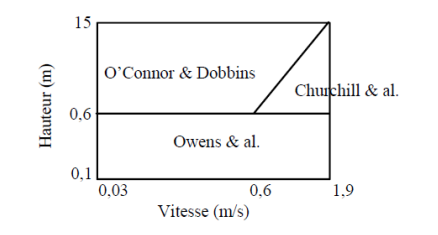
\includegraphics[width=8cm]{./graphics/k2diagram.png}\\
  \caption{choice of the K2 formula depending on hydrodynamics of the flow}\label{k2choice}
\end{figure}


 Since these formulae are valid for a temperature of 20${}^\circ$C, the value of K2 is corrected like:
\[K_2={\left(K_2\right)}_{20{}^\circ C}\ {\left(1.024\right)}^{T-20}\]


 The oxygen density at saturation Cs can be estimated using the temperature of water (at 20${}^\circ$C, Cs=9 mg/l). Hence if the temperature in the model is varying with time (for example when Thermic Module is activated), Cs can be estimated with different ways using the key-word \textbf{\textit{FORMULA FOR COMPUTING CS}} (default 0) which can have the following values:

\begin{itemize}
\item  0: constant value given by \textbf{\textit{O2 SATURATION DENSITY OF WATER (CS)}} (default = 11mg/l)

\item  1: Formula of Elmore \& Hayes:
\[C_s=14.652-0.41022T+0.00799T^2-7.7774.{10}^{-5}T^3\]

\item  2: Formula of Montgomery:
\[C_s=468/(31.6+T)\]
\end{itemize}

\item  Reaeration at weirs: for the O2 process, a reaeration of the water due to the existence of weirs is implemented. The water oxygen concentration is increased when crossing from one side of a weir to the other side. The raise of the concentration is managed through the key-words \textbf{\textit{WEIR REAERATION COEFFICIENT RS}} and \textbf{\textit{FORMULA FOR COMPUTING RS}} which can have 5 options (see \cite{El-Kadi2012} for theoretical details):
\begin{itemize}
\item  0: RS is constant, in this case RS is given by \textbf{\textit{WEIR REAERATION COEFFICIENT RS }}(default 1.)

\item  1: formula of Gameson 1

\item  2: formula of Gameson 2

\item  3: formula of WRL1

\item  4: formula of WRL2
\end{itemize}
\end{itemize}




\paragraph{  Organic load L}

 The evolution of the organic load density [L] in time is assumed to be with a first order law:
\begin{equation*}
 F([L]) = K_1 [L]
\end{equation*}
 Where $K_1$ is a constant that describes the kinetic of degradation of the organic load. It is given using the key-word \textbf{\textit{CONSTANT OF DEGRADATION OF ORGANIC LOAD K1}} (default 0.25 per day).  The organic load is in mgO$_2$/l.


\paragraph{ Ammoniacal load}

 The ammoniacal load $NH_4$, which is also consuming oxygen, has a density varying in time with a first order law given by:
\begin{equation*}
 F([NH{}_{4}]) = K_4 [NH{}_{4}]
\end{equation*}
 Where $K_4$ is a constant of nitrification kinetic. It is given by \textbf{\textit{CONSTANT OF NITRIFICATION KINETIC K4}}\textit{ }(default 0.35). In this module, $K_4$ is assumed to be constant and independent of remaining variables.


\paragraph{ Final source terms}

 The oxygen density is varying under the influence of sources with respect to the following law:
\begin{equation*}
F\left([O_2]\right)= K_2\left(C_s-[O_2]\right)-K_1\left[L\right]-K_4\left[NH_4\right]+P-R-\frac{BEN}{h}
\end{equation*}

\paragraph{ Example of steering file}

 To activate the water quality module we give here the set of key-words to include in the steering file of \telemac{2d}:
\begin{lstlisting}[language=bash]
/------------------------------------------------------
  WATER QUALITY
/------------------------------------------------------
WATER QUALITY           = YES
WAQ STEERING FILE    = 'waq\_steer.cas'
WAQ DICTIONARY         = 'waqtel.dico'
\end{lstlisting}
We give hereafter an example of WAQ steering file with the use of O${}_{2}$ process:
\begin{lstlisting}[language=bash]
/WAQ STEERING FILE
/---------------------------------------------------------
/GENERAL PARAMETERS:
/---------------------------------------------------------
WAQ CASE TITLE                = 'WAQ O2: VALIDATION CASE'
WATER DENSITY                 = 1000.
KINEMATIC WATER VISCOSITY     = 1.E-6
WATER QUALITY PROCESS         = 1
/   OPTIONS ARE :
/       1- O2 PROCESS
/       2- BIOMASS PROCESS
/       3- EUTRO PROCESS
/       4- MICROPOL PROCESS
/       5- THERMIC PROCESS
/-----------------------
//
// O2 PROCESS
//
/-----------------------
CONSTANT OF DEGRADATION OF ORGANIC LOAD K1 = 0.25
CONSTANT OF NITRIFICATION KINETIC K4       = 0.35
PHOTOSYNTHESIS P                           = 1.
VEGERAL RESPIRATION R                      = 0.06
WATER TEMPERATURE                          = 20.
/ In case of existence of weirs uncomment the following lines:
/WEIR REAERATION COEFFICIENT RS'
/FORMULA FOR COMPUTING RS'
//GIVES HOW TO CUMPUTE THE WEIR REAERATION COEFFICIENT RS
//OPTIONS ARE:
//  0- RS CONSTANT, IN THIS CASE RS=1.0
//  1- FORMULA OF GAMESON 1
//  2- FORMULA OF GAMESON 2
//  3- FORMULA OF WRL 1
//  4- FORMULA OF WRL2
/COEFFICIENTS A AND B FOR RS FORMULA'
\end{lstlisting}

\subsection{ The thermic module}
\label{subs:therm:mod}
 For a majority of water quality processes, the interaction with atmosphere is a key parameter. The neighboring conditions are taken into account through a meteorological file like the one described in section \ref{subs:meteo:file}. It is important to underline that the data contained in this file can vary depending on the considered case. The subroutine meteo can be edited by user to customize it to his specific model.

 The evolution of temperature of water is tightly linked to heat fluxes through the free surface. These fluxes (in W/m2) are of 5 natures:

\begin{itemize}
\item  Sun ray flux RS

\item  Atmospheric radiation flux RA

\item  Free surface radiation flux RE

\item  Advection heat flux CV

\item  Heat flux due to evaporation CE
\end{itemize}

 The final balance of (surface) source terms is given by
\[s_{surf}=RS+RA-RE-CV-CE\]
We will give a brief description for each of these terms, for more details see \cite{El-Kadi2012}. This surface source term is treated explicitly in \telemac{2d}, the following term is added in the explicit source term of advection-diffusion equation of tracer$\frac{S_{surf}}{\rho C_pH}$.


\paragraph{ Sun ray flux RS}

 Sun ray flux is simply provided in the meteo file. In a majority of cases, when no measurements are not available, this flux is estimated using the method of Perrin \& Brichambaut (\cite{El-Kadi2012}), which uses the cloud cover of the sky that varies during the day (function of time). So far, this flux is considered constant in space.  For more real cases, user is invited to use the ``heat exchange'' module (in folder sources/telemac3d). A sun ray flux varying in space, common between \telemac{2d} and \telemac{3d} will be implemented in next releases.


\paragraph{ Atmospheric radiation RA}

 The atmospheric radiation RA is estimated with meteorological data collected at the ground level. It takes into account energy exchanges with the ground, water (and energy) exchanges with the underground, etc. In this module, RA is estimated mainly by the air temperature, like:
\begin{equation*}
RA=e_{air}\sigma\left(T_{air}+273.15 \right)^4\left(1+k\left(\frac{c}{8}\right)^2 \right)
\end{equation*}
 Where $e_{air}$ is a calibrating coefficient given the key-word \textbf{\textit{COEFFICIENTS FOR CALIBRATING ATMOSPHERIC RADIATION} }(default 0.75). $\sigma$ is the constant of Stefan-Boltzmann (5.67.10${}^{-8}$ Wm${}^{-2}$K${}^{-4}$). Tair is air temperature given in the meteo file. k is coefficient that represents the nature of clouds, it has a mean value of 0.2 (key-word \textbf{\textit{COEFFICIENT OF CLOUDING RATE}}). However, it varies like indicated in Table \ref{tab:kcloud}.
\begin{table}
  \centering
  \begin{tabular}{|l|c|}
     \hline 
     Type of cloud & k \\
     \hline \hline
     Cirrus & 0.04 \\
     Cirro-stratus & 0.08 \\
     Altocumulus & 0.17 \\
     Altostratus & 0.2 \\
     Cumulus & 0.2 \\
     Stratus & 0.24\\
     \hline 
   \end{tabular}
  \caption{Values of k depending on cloud type}\label{tab:kcloud}
\end{table}



\paragraph{  Free surface radiation RE}

 The available water is assumed to be a grey body. Radiation generated by this grey body through the free surface is given by:
\begin{equation*}
RE=e_{eau}\sigma\left(T_{eau}+273.15 \right)^4
\end{equation*}
where T${}_{eau}$ is the mean water temperature in ${}^\circ$C. T${}_{eau}$ is given by the key-word \textbf{\textit{WATER TEMPERATURE}} (default 7${}^\circ$C). e${}_{eau}$ is a calibration coefficient which depends on the nature of the site and obstacles around it. This coefficient is given with \textbf{\textit{COEFFICIENTS FOR CALIBRATING SURFACE WATER RADIATION}} (default 0.97). For instance, for a narrow river with lots of trees on its banks, e${}_{eau}$ is around 0.97, for large rivers or lakes it is about 0.92.


\paragraph{ Advection heat flux CV}

 This flux is estimated empirically:
\begin{equation*}
CV=\rho_{air}Cp_{air}\left(a+bV \right)\left(T_{eau}-T_{air} \right)
\end{equation*}
 where $\rho_{air}$ is the air density obtained by ${\rho }_{air}=\ \frac{100\ P_{atm}}{\left(T_{air}+273.15\right)287}$ where P${}_{atm}$ is the atmospheric pressure, introduced in the meteo file or using the key-word \textit{VALUE OF ATMOSPHERIC PRESSURE} (default 100~000 Pa) (this is a key-word of \telemac{2d}). Cp${}_{air}$ is the air specific heat (J/kg${}^\circ$C) given by \textbf{\textit{AIR SPECIFIC HEAT}} (default 1002), V is the wind velocity (m/s) and a, b are empirical coefficients to be calibrated. Theirs values are very close to 0.0025, but they can be changed using \textbf{\textit{COEFFICIENTS OF AERATION FORMULA}} (default (0.002, 0.0012)).


\paragraph{ Evaporation heat flux CE}

 It is given by the following empirical formula:
\begin{equation*}
CE=L\rho_{air}\left(a+bV \right) \left(H^{sat}-H \right)
\end{equation*}
 where L=2500900-2365T${}_{water}$ is the vaporization latent heat (J/Kg), $H^{sat}=\frac{0.622P^{sat}_{vap}}{P_{atm}-0.378P^{sat}_{vap}}$ is the air specific moisture (humidity) at saturation (kg/kg), $H=\frac{0.622P_{vap}}{P_{atm}-0.378P_{vap}}$ is the specific humidity of air (kg/kg), P${}_{vap}$ is the partial pressure of water vapour in the air (hPa=10${}^{5}$Pa) which is given in the meteo file. $P^{sat}_{vap}$ is the partial pressure of water vapour at saturation (hPa) which is estimated with :
\begin{equation*}
P^{sat}_{vap}=6.11exp\left(\frac{17.27T_{eau}}{T_{eau}+237.3} \right)
\end{equation*}
 when H${}^{sat}<$H, the atmospheric radiation RA is corrected by multiplying it with 1.8.


\paragraph{ Example of steering file}

 To activate the water quality module we give here the set of key-words to include in the steering file of \telemac{2d}:
\begin{lstlisting}[language=bash]
/------------------------------------------------------
  WATER QUALITY
/------------------------------------------------------
WATER QUALITY           = YES
WAQ STEERING FILE    = 'waq\_steer.cas'
WAQ DICTIONARY         = 'waqtel.dico'
\end{lstlisting}
 We give hereafter an example of WAQ steering file with the use of Thermic process:
\begin{lstlisting}[language=bash]
/WAQ STEERING FILE
/--------------------------------------------------------------
/GENERAL PARAMETERS:
/--------------------------------------------------------------
WAQ CASE TITLE                = 'WAQ THERMIC: VALIDATION CASE'
WATER DENSITY                 = 1000.
KINEMATIC WATER VISCOSITY     = 1.E-6
WATER QUALITY PROCESS         = 5
/   OPTIONS ARE:
/       1- O2 PROCESS
/       2- BIOMASS PROCESS
/       3- EUTRO PROCESS
/       4- MICROPOL PROCESS
/       5- THERMIC PROCESS
/--------------------------------------------------------------
//
//THERMIC PROCESS
//
WATER SPECIFIC HEAT                                  = 4180.
AIR SPECIFIC HEAT                                    = 1002.
COEFFICIENTS OF AERATION FORMULA                = 0.0025;0.0025
COEFFICIENT OF CLOUDING RATE                         = 0.2
COEFFICIENTS FOR CALIBRATING ATMOSPHERIC RADIATION   = 0.85
COEFFICIENTS FOR CALIBRATING SURFACE WATER RADIATION = 0.97
\end{lstlisting}

%----------------------------------------------------------------------------------------
%	CHAPTER 12 : LAGRANGIAN TRANSPORT 
%----------------------------------------------------------------------------------------
\chapter{ PARTICLE TRANSPORT AND LAGRANGIAN DRIFTS}
\label{ch:part:transp}

\section{ Drogue Displacements}
\label{sec:drog:displ}
 During a hydrodynamic simulation, \telemac{2d} offers the possibility of monitoring the tracks followed by certain particles (drogues) introduced into the fluid from outflow points. The result is produced in the form of a Tecplot format file containing the various positions of the drogues in time, see paragraph \ref{subs:drog:output:file} for more details.

 Note that using this function provides more accurate results than using the particle tracking features of the post-processing tools. Contrary to \telemac{2d} for which monitoring floats is determined at each time step, the post-processing tools are based on the results file that is usually sampled much coarser. Since release 7.0 the management of drogues is modified to be coherent with other particle transport features of \telemac{2d} (oil spill and algae). Hereafter, we give the implementation details.

\subsection{ Input Files}
\label{subs:drog:inp:fil}
 In addition to the mandatory files for a classical \telemac{2d} model (steering, geometry boundary conditions), it is necessary to add a fortran file to run a particle transport case.

\subsection{ Steering file}
\label{subs:drog:steer:file}
 The steering file has to include the following key-words to account for drogue transport (for oil spill and algae, as well):

\begin{enumerate}
\item  The number of particles released: \textit{NUMBER OF DROGUES}, this is the maximum number used to dimension various arrays.

\item  The frequency of the drogues printout period: \textit{PRINTOUT PERIOD FOR DROGUES} \textit{;}

\item  The name of the output file (tecplot file) containing the drogue displacement: \textit{DROGUES FILE} (see section \ref{subs:drog:output:file});

\item  \telemac{2d} offers the possibility to introduce a stochastic diffusion coefficient. When setting the key-word \textit{STOCHASTIC DIFFUSION MODEL} =1 (default = 0), a stochastic model will generate stochastically a diffusion coefficient which is computed using the turbulent viscosity. If no turbulence is activated, this stochastic diffusion is not considered during the particle transport.
\end{enumerate}

\subsection{ Fortran file}
\label{subs:drog:fortr:file}
 Once the number of released drogues has been defined in the steering file, subroutine FLOT is used to define their positions and time of release. This is done by using the variable LT, which is the iteration step. This variable is used to release particles at a specific time. The subroutine ADD\_PARTICLE is then used to set the initial values of variables XFLOT, YFLOT and TAGFLOT, which are the two-dimensional position components and an identifier of the particle. An example of these changes can be found in subroutine FLOT (./sources/telemac2d). See also section \ref{sec:oil:spill:modell}.

 \textbf{Modifications to subroutine }FLOT\textbf{:}

\begin{enumerate}
\item \textbf{ }Use LT to define when to release particles

\item  Call ADD\_PARTICLE to define XFLOT, YFLOT and TAGFLOT
\end{enumerate}


\subsection{ Output file}
\label{subs:drog:output:file}
 Besides the classic result file, \telemac{2d} produces a specific output file for drogues. It is given by the key-word \textit{DROGUES FILE. }

 This file is a formatted file created by \telemac{2d} during the computation. It stores drogue positions in TECPLOT format. To visualize the drogue positions with Tecplot software, the user must:

\begin{enumerate}
\item  Use the File$>$Load Data File(s) command to load the 2D RESULT FILE

\item  Use the File$>$Load Data File(s) command to load the Tecplot drogue file
\end{enumerate}

\begin{WarningBlock}{Warning:}
 In order to add the Tecplot DROGUE FILE to Telemac result data that was already loaded, select ``Add to current data'' set in the \textbf{Load Data File Warning dialogue} (cf. Figure \ref{fig:load:df}). The Load Data File Warning dialogue will appear after you have selected the file and zones and/or variables to load.
\end{WarningBlock}
\begin{figure}
\centering
 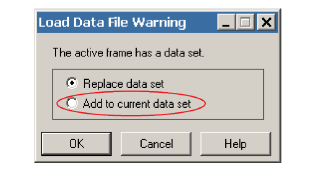
\includegraphics[width=2.77in, height=1.70in, keepaspectratio=false]{./graphics/warning1.png}
\label{fig:load:df}
\end{figure}

 \textbf{Change the drogue output format:}

 It is possible to develop a new drogue output format. This must be done in the subroutine DERIVE. A Fortran file including the subroutine DERIVE with the new format definition for the DROGUE FILE needs to be added with the input files.


\section{ Algae bloom modelling}
\label{sec:algae:bloom}
 Since release 6.3, \telemac{2d} offers the possibility to simulate algae bloom transport. Theoretical aspects about algae physics and modelization can be found in Joly \cite{Joly2011}.


\subsection{Input files}

 Input files for algae bloom modelling are the same than for drogues.


\subsection{ Steering file}

 The steering file has to include the following key-words to account for an algae bloom propagation model:

\begin{itemize}
\item  The number of particle released: \textit{NUMBER OF DROGUES};

\item  The frequency of the algae printout period: \textit{PRINTOUT PERIOD FOR DROGUES};

\item  The name of the output file (tecplot file) containing the drogue displacement: \textit{DROGUES FILE} (see section \ref{subs:drog:output:file});

\item  The option setting the particles as algae: \textit{ALGAE TRANSPORT MODEL=YES} (default\textit{ = NO});

\item  The type of algae particles considered \textit{ALGAE TYPE} (default 1). The different choices are:

\begin{enumerate}
\item Sphere,

\item Iridaea Flaccida,

\item Pelvetiopsis Limitata,

\item Gigartina Leptorhynchos
\end{enumerate}

\item  The physical properties of the algae (diameter, density and thickness):

\begin{itemize}
\item  \textit{DIAMETER OF ALGAE} (default = 0.1);

\item  \textit{DENSITY OF ALGAE} (default = 1050);

\item  \textit{THICKNESS OF ALGAE} (default = 0.01).
\end{itemize}
\end{itemize}

\begin{WarningBlock}{Warning:}

\begin{itemize}
\item  Even though some of the previous keywords make references to drogues, they are also used for algae blooms.

\item  To use the algae particle transport module it is necessary to use the k-$\epsilon$ turbulence model, i.e. the option \textit{TURBULENCE MODEL = 3} needs to be set in the steering file.
\end{itemize}
\end{WarningBlock}

\subsection{Fortran file}

 Once algae transport has been defined in the steering file, the subroutine FLOT is used to define the position and time of release. This is done by defining the variable ALGAE\_START and using the variable LT to release particles. In addition the subroutine ADD\_PARTICLE is used to set the initial values of variables XFLOT, YFLOT and TAGFLOT, which are the two-dimensional position components and an identifier of the particle. An example how to use FLOT to release algae particles is put in comments within the subroutine FLOT.

 \textbf{Modifications to subroutine for algae transport}

\begin{enumerate}
\item Add the command USE ALGAE\_TRANSP at the beginning of the routine

\item  Define ALGAE\_START, which will be used as the release time of the algae (so far a simple time release is allowed)

\item  Use LT to release particles

\item  Call ADD\_PARTICLE to define XFLOT, YFLOT and TAGFLOT
\end{enumerate}

\begin{WarningBlock}{Warning:}
\begin{itemize}
\item  ALGAE\_START needs to be greater or equal to 1

\item  So far, it is possible to achieve a unique release of algae. To do multiple releases (in different times), futher developments are necessary.
\end{itemize}
\end{WarningBlock}

\subsection{ Output files}

 Likewise for drogues, see \ref{subs:drog:output:file}.


\section{ Oil spill modelling}
\label{sec:oil:spill:modell}
 A new feature has been added to \telemac{2d} (and 3D) that allows the simulation of oil spill problems. These developments are based on the work of Goeury \cite{goeury2012}.


\subsection{ Input files}

 In addition to the minimum set of input files necessary to run a \telemac{2d} case, an oil spill computation needs also an oil spill steering file. Furthermore, to run oil spill model a FORTRAN file including the routine OIL\_FLOT needs to be added.


\subsection{ Steering file}

 The following essential information should be specified in the \telemac{} steering file to run an oil spill propagation model:

\begin{itemize}
\item  The use of the oil spill model must be declared: \textit{OIL SPILL MODEL = YES} (default\textit{ = NO});

\item  The name of the oil spill steering file which contains the oil characteristics: \textit{OIL SPILL STEERING FILE};

\item  The number of oil particles to be released during the oil spill episode: \textit{NUMBER OF DROGUES};

\item  The frequency of the drogues printout period: \textit{PRINTOUT PERIOD FOR DROGUES}; 

\item  The name of the Tecplot file containing the oil displacement: \textit{DROGUES FILE}.
\end{itemize}

\begin{WarningBlock}{Warning:}
\begin{itemize}
\item  Even though some of the previous keywords make references to drogues, they are also used for algae blooms and oil spills.

 With the oil spill module, it is possible to take into account the transport of soluble oil components in water (whose presence has no effect on the hydrodynamics). These may or may not be diffused within the flow but their characteristics have to be defined in the \textit{OILSPILL STEERING FILE.} If these components are allowed to diffuse in the flow they are then treated with the tracer transport computations of \telemac{2d}. This implies that the logical keyword \textit{TRACER} is set to \textit{YES} and the \textit{NUMBER OF TRACER} must be set to the number of the oil soluble components. In addition, \textit{TRACER} keywords, enunciated in the Chapter \ref{ch:tra:trans} can be specified.

\item If the number of oil components dissolved in water is greater than 1, the result file can contain the sum of dissolved oil concentrations. The user must only add the variable for graphic printout N:

\textit{VARIABLES FOR GRAPHIC PRINTOUTS: '....,N'}

With the variable for graphic printout \textbf{\textit{N}}, be careful not to have private tables or change the table PRIVE1 in the subroutine PRERES\_TELEMAC2D.f by the table PRIVEX (where X is the number chosen by the user).
\end{itemize}
\end{WarningBlock}

\subsection{ Oil spill steering file}

 As seen previously, the \textit{OIL SPILL STEERING FILE }name is given by the user in the \telemac steering file. This file contains all information on oil calculation based on the composition considered by the user:

\begin{enumerate}
\item  The number of non-soluble components in oil,

\item  The parameters of these components such as the mass fraction (\%) and boiling point of each component (K),

\item  The number of soluble components in oil,

\item  The parameters of these components such as the mass fraction (\%), boiling point of each component (K), solubility (K${}_{g}$.m${}^{-3}$) and the mass transfer coefficient of the dissolution and volatilization phenomena (m.s${}^{-1}$),

\item  The oil density,

\item  The oil viscosity (m${}^{2}$.s${}^{-1}$),

\item  The volume of the spilled oil (m${}^{3}$),

\item  The water surface temperature (K),

\item  The spreading model chosen by the user:

\begin{enumerate}
\item  Fay's model,

\item  Migr'Hycar model,

\item  Constant area model.
\end{enumerate}
\end{enumerate}

\begin{WarningBlock}{Warning:}
\begin{itemize}
\item The parameters of soluble (or non-soluble) components need to be informed only if the number of these components is not null,

\item  If the sum of all mass fraction components is not equal to 1, the run is interrupted and an error message is displayed:

 ''WARNING::THE SUM OF EACH COMPONENT MASS FRACTION IS NOT EQUAL TO 1.''

 ``PLEASE, MODIFY THE INPUT STEERING FILE''
\end{itemize}
\end{WarningBlock}

An example of the oil spill steering file is given.
\begin{lstlisting}[language=bash]
NUMBER OF UNSOLUBLE COMPONENTS IN OIL
6
UNSOLUBLE COMPONENTS PARAMETERS (FRAC MASS, TEB)
5.1D-02    ,402.32D0
9.2D-02    ,428.37D0
3.16D-01   ,458.37D0
3.5156D-01    ,503.37D0
8.5D-02       ,543.37D0
9.4D-02       ,628.37D0
NUMBER OF SOLUBLE COMPONENTS IN OIL 
4
SOLUBLE COMPONENTS PARAMETERS(FRAC MASS, TEB, SOL, KDISS, KVOL)
1.D-02   ,497.05D0,  0.018D0   , 1.25D-05 ,5.0D-05
3.2D-02  ,551.52D0,  0.00176D0 , 5.63D-06 ,1.51D-05
1.D-04   ,674.68D0,  2.0D-04   , 2.D-06   ,4.085D-07
2.D-05   ,728.15D0,  1.33D-06  , 1.33D-06 ,1.20D-07
OIL DENSITY
830.D0
OIL VISCOSITY
4.2D-06
OIL SPILL VOLUME
2.02D-05
WATER TEMPERATURE
292.05D0
SPREADING MODEL(1=FAY'S MODEL,2=MIGR'HYCAR MODEL,3=CONSTANT AREA)
2
\end{lstlisting}
If in the oil spill steering file, the SPREADING MODEL is set to 3, two lines must be added to the previous example:
\begin{lstlisting}[language=bash]
CONSTANT AREA VALUE CHOSEN BY THE USER FOR EACH OIL PARTICLE
1 
/example if the user wants area particle equal to 1 m2
\end{lstlisting}
\subsection{ The oil\_flot subroutine}

 After inserting the OIL\_FLOT subroutine in the FORTRAN file, the user must modify it in order to indicate the release time step, together with the coordinates of the release point. If the release point coordinates are outside the domain, the run is interrupted and an error message is displayed. In addition, if a particle leaves the domain during the simulation, it is of course no longer monitored but its previous track remains in the results file for consultation.

 An example of modifications in the OIL\_FLOT subroutine is given.

 The release time step in the first condition statement and the coordinates of the release point must be changed:
\begin{lstlisting}[language=TelFortran]
...
IF(LT.EQ.10000)THEN
  NUM_GLO=0
  NUM_MAX=0
  NUM_LOC=0
  COORD_X=0.D0
  COORD_Y=0.D0
  NUM_MAX=INT(SQRT(REAL(NFLOT_MAX)))
  DO K=1,NUM_MAX
    DO J=1,NUM_MAX
      COORD_X=336000.D0+REAL(J)
      COORD_Y=371000.D0+REAL(K)
      NUM_GLO=NUM_GLO+1
      NFLOT_OIL=0
      CALL ADD_PARTICLE(COORD_X,COORD_Y,0.D0,NUM_GLO,NFLOT_OIL,
&                       1,XFLOT,YFLOT,YFLOT,TAGFLO,
&                       SHPFLO,SHPFLO,ELTFLO,ELTFLO,MESH,1,
&                       0.D0,0.D0,0.D0,0.D0,0,0)
...
    END DO
  ENDDO
END IF
\end{lstlisting}

\subsection{ Output files}

 There are no additional output files provided than for drogue transport.

\begin{WarningBlock}{Warning:}
 If the user wants to develop a new drogue output format for oil spill, he must edit subroutine OIL\_DERIVE.f and not the subroutine DERIVE.f used for the drogue and algae transport.
\end{WarningBlock}

\section{ Lagrangian drifts}
\label{sec:lagr:drifts}

\subsection{ Input files}

 Computing Lagrangian drifts involves computing the displacement of all mesh points between two given instants. Typically, these two instants may be two consecutive high tides.

 To run such a computation, it is necessary to program the steering file and FORTRAN file.

 In the steering file, the user must firstly provide the number of drifts required using the keyword \textit{NUMBER OF LAGRANGIAN DRIFTS} (default value 0). This value corresponds to the number of pairs (starting and ending times) for which the Lagrangian drifts are computed. Secondly, the user must include the letters A and G in the list assigned to the keyword \textit{VARIABLES FOR GRAPHIC PRINTOUTS}. These two letters correspond to the drift displacements along X and Y.

 As far as the FORTRAN file is concerned, the user must insert the LAGRAN subroutine, in which it is necessary to define the instants at which each computation is to start and end, in the form of time step numbers.

 The drift computation results are stored directly in the \telemac{2d} results file in the form of two scalar variables entitled DRIFT\_ALONG\_X and DRIFT\_ALONG\_Y. Given the possible discretization that may occur in printing out graphical results, the rule for introduction in the results file is the following:

\begin{itemize}
\item  If none of the drift computations is completed at the time step considered, the two variables are set to zero.

\item  Otherwise, the two variables contain the results of the most recently completed drift computation.
\end{itemize}

 This means on one hand that two drifts may not be completed at the same time step, and on the other hand that between two ends of drift computations, a record must be made in the results file (otherwise the result of the first computation is lost).

 Lastly, if a drift leaves the domain, the corresponding computation is interrupted and the result reset at zero for this node.


\subsection{ Output files}

 The result is produced in the form of a Serafin format file containing the various positions of the lagrangian drifts in the form of a degenerated mesh.



  The following example (steering file and FORTRAN file) carries out two drift computations. The first begins at time step 10 and finishes at time step 50. The second begins at time step 15 and finishes at time step 40.

  In the steering file:
\begin{lstlisting}[language=bash]
NUMBER OF LAGRANGIAN DRIFTS     = 2
VARIABLES FOR GRAPHIC PRINTOUTS = 'U,V,H,A,G'
GRAPHIC PRINTOUT PERIOD         = 1
\end{lstlisting}
  In the LAGRAN subroutine of the FORTRAN file:
\begin{lstlisting}[language=TelFortran]
DEBLAG(1) = 10
FINLAG(1) = 50
DEBLAG(2) = 15
FINLAG(2) = 40
\end{lstlisting}
 In this example, the variables DRIFT\_ALONG\_X and DRIFT\_ALONG\_Y of the results file will contain the following values:

\begin{itemize}
\item  From time steps 1 to 39: 0 values (no finished drift computation).

\item  From time steps 40 to 49: results of the second drift computation.

\item  Time step 50: results of the first drift computation.
\end{itemize}

 NOTE: Lagrangian drifts are not yet implemented for parallelism.


%----------------------------------------------------------------------------------------
%	CHAPTER 13 : CONSTRUCTION WORKS
%----------------------------------------------------------------------------------------

\chapter{  CONSTRUCTION WORKS MODELLING}
\label{ch:constr:wm}

\section{ Weirs}
\label{sec:weirs}
 Weirs are considered as linear singularities. Their use is possible in parallel computing (since release 6.2). The number of weirs is specified by the keyword \textit{NUMBER OF WEIRS} (default value 0). Information about weirs is given in the \textit{WEIRS DATA FILE}.

 A weir must be prepared in the mesh and consists of two boundary lines which are actually linked by the weir. In principle, these boundaries should be sufficiently far apart, upstream and downstream of the weir. The upstream and 
downstream boundary points should correspond 1 to 1, and the distance between two points should be the same on both sides. The following file gives an example of two weirs (the comments are part of the file):
\begin{lstlisting}[language=bash]
Nb of culverts  Option for tangential velocity
      2                    0
---------------------------- singularity 1
Nb of points for 1 side
11
Points side 1
71 72 73 74 75 76 77 78 79 80 41
Points side 2
21 20 19 18 17 16 15 14 13 12 11
level of the dike
1.8 1.8 1.8 1.8 1.8 1.8 1.8 1.8 1.8 1.8 1.8
flowrate coefficients
 .4  .4  .4  .4  .4  .4  .4  .4  .4  .4  .4
---------------------------- singularity 2
Nb of points
11
Points side 1
111 112 113 114 115 116 117 118 119 120 81
Points side 2
61 60 59 58 57 56 55 54 53 52 51
Level of the dike
1.6 1.6 1.6 1.6 1.6 1.6 1.6 1.6 1.6 1.6 1.6
flowrate coefficient
 .4  .4  .4  .4  .4  .4  .4  .4  .4  .4  .4
\end{lstlisting}

 Line 2 indicates the number of weirs and then an option for the treatment of tangential velocities on the weir, with the following meaning:

\begin{enumerate}
\item [\nonumber] 0: the velocities are null (recommended option),

\item [\nonumber] 1: the velocities will be calculated with the Ch\'{e}zy formula (as a function of the local free surface slope).
\end{enumerate}

 For each weir, it is then necessary to indicate: the number of points for the first side of the weir (line 5 for the first weir) and the list of their global numbers (line 7 for the first weir). Note, that before and for release 6.1, the numbering to provide was not the global one but the local numbering of the boundary defined in the boundary conditions file. However, it is necessary to provide the weirs number in the order of the boundary points.

 The numbers of their twin points on side 2 should be given on line 9 in the reverse order. On line 11, the level of the weir is specified for each couple of points and at line 13 the discharge coefficient noted m. All these data are repeated for all weirs.

 The formulae used to calculate the discharge for each point are the following:

\begin{enumerate}
\item  Unsubmerged weir: $Q=\mu \sqrt{2g}\ {\left(upstream-threshold\right)}^{\frac{3}{2}}$

\item  Submerged weir:
\[Q=\ {\left(\frac{2}{3}\sqrt{\frac{1}{3}}\right)}^{-1}\mu \sqrt{2g}\left(downstream-threshold\right)\sqrt{\left(upstream-threshold\right)}\]

\item  The weir is not submerged if:
\[upstream\ level<\frac{threshold\ level+2*upstream\ level}{3}\]
\end{enumerate}
Depending on the shape and roughness of the weir, the value of ${\kern 1pt} \mu $ is between 0.4 and 0.5. However, the above formulae neglect the velocity of the upstream head in the computation. If this is not the case, the value of ${\kern 1pt} \mu $ may be higher.

 If the user wants to modify the different laws, it is possible to modify the appropriate subroutines (LOIDEN.f and LOINOY.f).

\section{ Culverts}
\label{sec:culverts}
 As for weirs, the keyword \textit{NUMBER OF CULVERTS} specifies the number of culverts to be treated. Culverts are described as couples of points between which flow may occur, as a function of the respective water level at these points. Since release 6.2 of \telemac{2d}, it is no longer necessary to describe each culvert inflow and outflow as a source point.

 Information about culvert characteristics is stored in the \textit{CULVERT DATA FILE}.

 The following file gives an example of a culvert:
\begin{lstlisting}[language=bash]
 Relaxation   Number of siphons
   0.2              1
 I1   I2  d1  d2   CE1  CE2  CS1   CS2   S12  L12  z1   z2  a1   a2
 531 562  0.  90.  0.5  0.5  1.0   1.0   20.  0.2  0.3  0.1  0.  90.
\end{lstlisting}
 The relaxation coefficient is initially used to prescribe the discharge in the culvert on a progressive basis in order to avoid the formation of an eddy. Relaxation, at T time, between result computed at time T and result computed at previous time step.. A relaxation coefficient of 0.2 means that 20\% of time T result is mixed with 80\% of the previous result. I1 and I2 are the numbers of each end of the culvert in the global point numbering system.

 The culvert discharge is given by the following formula (with flow going from 1 to 2):
\[Q{\kern 1pt} {\kern 1pt} {\kern 1pt} {\kern 1pt} {\kern 1pt} ={\kern 1pt} {\kern 1pt} {\kern 1pt} {\kern 1pt} {\kern 1pt} S_{12} {\kern 1pt} {\kern 1pt} {\kern 1pt} \left({\kern 1pt} \frac{2g{\kern 1pt} {\kern 1pt} {\kern 1pt} (upstream{\kern 1pt} {\kern 1pt} {\kern 1pt} {\kern 1pt} level{\kern 1pt} {\kern 1pt} {\kern 1pt} {\kern 1pt} {\kern 1pt} -{\kern 1pt} {\kern 1pt} {\kern 1pt} {\kern 1pt} downstream{\kern 1pt} {\kern 1pt} {\kern 1pt} {\kern 1pt} {\kern 1pt} level)}{CS_{2} {\kern 1pt} {\kern 1pt} +{\kern 1pt} {\kern 1pt} {\kern 1pt} CE_{1} {\kern 1pt} {\kern 1pt} {\kern 1pt} {\kern 1pt} +{\kern 1pt} {\kern 1pt} {\kern 1pt} {\kern 1pt} L_{12} } \right)\]
S${}_{12}$ is the cross-section of the pipe. CS${}_{1}$ and CS${}_{2}$ are the head loss coefficients of 1 and 2 when they are operating as outlets. CE${}_{1}$ and CE${}_{2}$ are the head loss coefficients of 1 and 2 when they are operating as inlets. L${}_{12}$ is the linear head loss coefficient, generally equal to $\lambda {\kern 1pt} {\kern 1pt} {\kern 1pt} {\kern 1pt} {\kern 1pt} \frac{L}{D} $ where L is the length of the pipe, D its diameter and l the friction coefficient.

 z${}_{1}$ and z${}_{2}$ are the levels of the tapers.

 a${}_{1}$ and a${}_{2}$ are the angles that the pipe makes with respect to the bottom, in degrees. For a vertical intake, the angle with the bottom will therefore be 90${}^\circ$.

 d${}_{1}$ and d${}_{2}$ are the angles with respect to the x axis. They are used to account for the current direction at source or sink point that or not normal to bottom.


\section{ Tubes}
\label{sec:tubes}
 Tubes allow to model construction works that are likely to switch from free surface flow to close-conduit flow during the simulation (discharge construction work under a dike, a bridge, etc.). As for weirs, the keyword \textit{NUMBER OF CULVERTS} specifies the number of tubes to be treated. Tubes are described as couples of points between which flow may occur, as a function of the respective water level at these points. Contrary to culverts, the flow direction is automatically computed as a function of inflow and outflow points of the tube.
 Information about culvert characteristics is stored in the \textit{TUBES DATA FILE}.
 The following file gives an example of two tubes:
\begin{lstlisting}[language=bash]
 Relaxation
     0.05
 I1   I2   Ce1  Ce2  Cs1  Cs2  Lrg  Hau  Clp  L12   z1  z2
 2566 2705 0.5  0.5  1.   1.   2.5  1.5  0    0.2   1.0 1.0
 2520 2659 0.5  0.5  1.   1.   2.5  1.5  0    0.2   1.0 1.0
\end{lstlisting}
 The relaxation coefficient is used to prescribe the discharge in the tube on a progressive basis in order to avoid the formation of an eddy. I1 and I2 are the numbers of each end of the tube in the global point numbering system.

 CE${}_{1}$ and CE${}_{2}$ are the head loss coefficients when the considered point is operating as inlet.

 CS${}_{1}$ and CS${}_{2}$ are the head loss coefficients when the considered point is operating as outlet.

 L${}_{rg }$is the width of the construction work (in meter).

 H${}_{au}$${}_{ }$is the height of the construction work (in meter).

 C${}_{lp}$${}_{ }$is an indicator allowing specifying a check valve behaviour. The different possibilities are:

\begin{enumerate}
\item  [\nonumber] 0 : Flow in both direction is allowed,

\item [\nonumber] 1 : Only flow from point 1 to point 2 is allowed,

\item [\nonumber] 2 : Only flow from point 2 to point 1 is allowed,

\item [\nonumber] 3 : No flow allowed (this feature allows to disable the tube without having to suppress it)
\end{enumerate}

 L${}_{12}$ is the linear head loss coefficient, generally equal to $\lambda {\kern 1pt} {\kern 1pt} {\kern 1pt} {\kern 1pt} {\kern 1pt} \frac{L}{D} $ where L is the length of the pipe, D its diameter and $\lambda$ the friction coefficient.

 z${}_{1}$ and z${}_{2}$ are the levels of the tapers.


\section{ Dykes breaches}
\label{sec:dykes}
 \telemac{2d} allows simulating dikes breaching by suddenly or gradually lowering the altitude of some points. This feature is enabled using the logical keyword \textit{BREACH}. The description of the breaching process is provided in the file specified by the keyword \textit{BREACHES DATA FILE}.

 In the current release, 3 types of breaching process are available:

\begin{itemize}
\item  at a given time,

\item  when the water level above the dike reaches a given value,

\item  when the water level at a given point reaches a certain value.
\end{itemize}

 The breaching zone is defined by a polyline of several points associated to a bandwidth. The final situation is characterized by a bottom altitude that will be reached by all the points located in the breaching zone. If after the dike breaching, the bottom level is not constant, it is thus necessary to divide the dike into several breaching polylines.

 Since release 7.0, it is possible to take into account a lateral growth of the breach (dike opening by widening). Old breaching processes are not affected by this new feature. However, the breaches file is modified as follows:

\begin{itemize}
\item  addition of two new lines for selecting breach opening option. These two lines -- comment line and the value for the option -- come after the breach duration. The options are selected using:
\begin{enumerate}
\item [\nonumber] 1: for dike opening by bottom lowering (the old implementation)

\item [\nonumber] 2: for dike opening by widening (the newly added option)

\end{enumerate}
\item  the width of polygon defining breach is given for each breach
\end{itemize}

 A commented example of breaches data file is provided below. This example is taken from the test case telemac2d/breach.

\begin{lstlisting}[language=bash]
# Number of breaches
3
# Bandwidth of the polyline defining the breach
15.0
# Upstream breach definition
# Width of Polygon defining the breaches
25.0
# Option for the breaching process
2
# Duration of the breaching process (0.0 = instant opening)
0.0
# option of lateral growth
#(1= bottom lowering, 2=dike opening by widening)
2
# Final bottom altitude of the breach
5.9
# Control level of breach 
#(breach exist if water level exceed this value)
7.2
# Number of points of the polyline
4
# Description of the polyline
2000.0 37.5
2041.0 37.5
2082.0 37.5
2100.0 37.5
# Central breach definition
# Width of Polygon defining the breaches
20.0
# Option for the breaching process
3
# Duration of the breaching process (0.0 = instant opening)
300.0
# Option of lateral growth
# (1= bottom lowering, 2=dike opening by widening)
1
# Final bottom altitude of the breach
5.5
# Number (global mesh) of the point controlling the breaching
9406
# Water level initiating the breaching process
6.0
# Number of points of the polyline
4
# Description of the polyline
2450.0 37.5
2500.0 37.5
2520.0 37.5
2550.0 37.5
# Downstream breach definition
# Width of Polygon defining the breach
10.0
# Option for the breaching process
1
# Start time of the breaching process
2000.0
# Duration of the breaching process (0.0 = instant opening)
600.0
# Option of lateral growth
# (1= bottom lowering, 2= opening by widening)
1
# Final bottom altitude of the breach
5.0
# Number of points on the dike axis where the breach will appear
4
# Description of the polyline
2900.0 37.5
2920.0 37.5
2950.0 37.5
3000.0 37.5
\end{lstlisting}

%----------------------------------------------------------------------------------------
%	CHAPTER 14 : OTHER CONFIGURATIONS
%----------------------------------------------------------------------------------------

\chapter{  OTHER CONFIGURATIONS}
\label{ch:oth:conf}

\section{ Modification of bottom topography (CORFON)}
\label{sec:mod:bott:topo}
 Bottom topography may be introduced at various levels, as was stated in section \ref{subs:topo:bathy:data}.

\telemac{2d} offers the possibility of modifying the bottom topography at the start of a computation using the CORFON subroutine. This is called up once at the start of the computation and enables the value of variable ZF to be modified at each point of the mesh. To do this, a number of variables such as the point coordinates, the element surface value, connectivity table, etc. are made available to the user.

 By default, the CORFON subroutine carries out a number of bottom smoothings equal to FILTER, i.e. equal to the number specified by the keyword \textit{BOTTOM SMOOTHINGS}.

 The CORFON subroutine is not called up if a computation is being continued. This avoids having to carry out several bottom smoothings or modify the bottom topography during the computation.


\section{ Modifying coordinates (CORRXY)}

 \telemac{2d} also offers the possibility of modifying the mesh point coordinates at the start of a computation. This means, for example, that it is possible to change the scale (from that of a reduced-scale model to that of the real object), rotate or shift the object.

 The modification is made in the CORRXY subroutine (BIEF library), which is called up at the start of the computation. This subroutine is empty by default and gives an example of programming concerning a change of scale and origin, in the form of commented statements.

 It is also possible to specify the coordinates of the origin point of the mesh. This is done using the keyword \textit{ORIGIN COORDINATES} which specify 2 integers. These 2 integers will be transmitted to the results file in the Serafin format, for a use by post-processors for superimposition of results with digital maps (coordinates in meshes may be reduced to avoid large real numbers). These 2 integers may also be used in subroutines under the names I\_ORIG and J\_ORIG. Otherwise they are not yet used.


\section{ Spherical coordinates (LATITU) }
\label{sec:spher:coord:LATI}
 If a simulation is being performed over a large domain, \telemac{2d} offers the possibility of running the computation with spherical coordinates.

 This option is activated when the keyword \textit{SPHERICAL COORDINATES} is positioned at YES (default value NO). In this case, \telemac{2d} calls a subroutine named LATITULATITU at the beginning of the computation. This calculates a set of tables depending on the latitude of each point. To do this, it uses the Cartesian coordinates of each point provided in the geometry file, and the latitude of the point of origin of the mesh provided by the user in the steering file with the keyword \textit{LATITUDE OF ORIGIN POINT}.

 By default, \telemac{2d} assumes that the mesh coordinates are given Cartesian coordinates. User can change this choice by using the keyword SPATIAL PROJECTION TYPE (default 1 which corresponds to Cartesian coordinates). Indeed, when choosing the value 2, the coordinates are considered in accordance with Mercator's projection. The value 3, the mesh has to be in longitude-latitude (in degrees!). It is important to notice here that, if option SPHERICAL COORDINATES=YES, SPATIAL PROJECTION TYPE has to be 2 or 3.

 The LATITU subroutine (BIEF library) may be modified by the user to introduce any other latitude-dependent computation.


\section{ Adding new variables (NOMVAR\_TELEMAC2D and PRERES\_TELEMAC2D)}

 A standard feature of \telemac{2d} is the storage of certain computed variables. In certain cases, the user may wish to compute other variables and insert them in the results file (the number of variables is currently limited to four).

 \telemac{2d} has a numbering system in which, for example, the array containing the Froude number has the number 7. The new variables created by the user may have the numbers 23, 24, 25 and 26.

 In the same way, each variable is identified by a letter in the keyword \textit{VARIABLES FOR GRAPHIC PRINTOUTS}. The new variables are identified by the letters N, O, R and Z, which correspond respectively to the numbers 23, 24, 25 and 26.

 At the end of NOMVAR\_TELEMAC2D, it is possible to change the abbreviations (mnemonics) used for the keywords \textit{VARIABLES FOR GRAPHIC PRINTOUTS} and \textit{VARIABLES FOR LISTING PRINTOUTS}. Sequences of 8 letters may be used. Consequently, the variables must be separated by spaces, commas or semi-colons in the keywords, e.g.:

 \textit{VARIABLES FOR GRAPHIC PRINTOUTS:'U,V,H;B'}

 In the software data structure, these four variables correspond to the tables PRIVE\%ADR(1)\%P\%R(X), PRIVE\%ADR(2)\%P\%R(X), PRIVE\%ADR(3)\%P\%R(X) and PRIVE\%ADR(4)\%P\%R(X) PRIVE (in which X is the number of points in the mesh). These may be used in several places in the programming, like all TELEMAC variables. For example, they may be used in the subroutines CORRXY, CORSTR, BORD, etc. If a PRIVE table is used for programming a case, it is essential to check the value of the keyword \textit{NUMBER OF PRIVATE ARRAYS}. This value fixes the number of tables used (0, 1, 2, 3 or more) and then determines the amount of memory space required. The user can also access the tables via the aliases PRIVE1, PRIVE2, PRIVE3 and PRIVE4.

 An example of programming using the second PRIVE table is given below. It is being initialized with the value 10.
\begin{lstlisting}[language=TelFortran]
 DO I=1,NPOIN   
   PRIVE%ADR(2)\%P\%R(I) = 10.D0
 ENDDO
\end{lstlisting}
 New variables are programmed in two stages:

\begin{enumerate}
\item  Firstly, it is necessary to define the name of these new variables by filling in the NOMVAR\_TELEMAC2D subroutine. This consists of two equivalent structures, one for English and the other for French. Each structure defines the name of the variables in the results file that is to be generated and then the name of the variables to be read from the previous computation if this is a continuation. This subroutine may also be modified when, for example, a file generated with the English version of \telemac{2d}  is to be continued with the French version. In this case, the TEXTPR table of the French part of the subroutine must contain the English names of the variables.

\item  Secondly, it is necessary to modify the PRERES\_TELEMAC2D subroutine in order to introduce the computation of the new variable(s). The variables LEO, SORLEO, IMP, SORIMP are also used to determine whether the variable is to be printed in the printout file or in the results file at the time step in question.
\end{enumerate}


\section{ Array modification or initialization}

 When programming \telemac{2d} subroutines, it is sometimes necessary to initialize a table or memory space to a particular value. To do that, the BIEF library furnishes a subroutine called FILPOL that lets the user modify or initialize tables in particular mesh areas.

 A call of the type CALL FILPOL (F,C, XSOM, YSOM, NSOM, MESH) fills table F with the C value in the convex polygon defined by NSOM nodes (coordinates XSOM, YSOM). The variable MESH is needed for the FILPOL subroutine but have no meaning for the user.


\section{ Validating a computation (VALIDA) }

 The structure of the \telemac{2d} software offers a point of entry for validating a computation, in the form of a subroutine named VALIDA, which has to be filled by the user in accordance with each particular case. Validation may be carried out either with respect to a reference file (which is therefore a file of results from the same computation that is taken as reference, the name of which is supplied by the keyword \textit{REFERENCE FILE}), or with respect to an analytical solution that must then be programmed entirely by the user.

 When using a reference file, the keyword \textit{REFERENCE FILE FORMAT} specifies the format of this binary file (SERAFIN by default).

 The VALIDA subroutine is called at each time step when the keyword \textit{VALIDATION} has the value YES, enabling a comparison to be made with the analytical solution at each time step. By default, the VALIDA subroutine only makes a comparison with the last time step. The results of this comparison are given in the control listing.


\section{ Changing the type of a boundary condition (PROPIN\_TELEMAC2D)}
\label{sec:chang:type:bc:propin}
 During a simulation, the type of boundary condition is generally fixed and, in the case of \telemac{2d}, is provided by the boundary conditions file. However, in certain cases, it may be necessary to change the type of boundary conditions during the computation (section of a river subject to tidal effects where the current alternates, for instance).

 This change in boundary condition type must be made in the PROPIN\_TELEMAC2D subroutine.

 N.B: modifying PROPIN\_TELEMAC2D is a difficult operation and must be done with great care!


\section{ Coupling}

 The principle of coupling two (or more) simulation modules involves running the two calculations simultaneously and exchanging the various results at each time step. For example, the following principle is used to link a hydrodynamic module and a sediment transport module:

\begin{itemize}
\item  The two codes perform the calculation at the initial instant with the same information (in particular the mesh and bottom topography).

\item  The hydrodynamic code runs a time step and calculates the depth of water and velocity components. It provides this information to the sediment transport code.

\item  The sediment transport code uses this information to run the solid transport calculation over a time step and thus calculates a change in the bottom.

\item  The new bottom value is then taken into account by the hydrodynamic module at the next time step, and so on.
\end{itemize}

 Two modules can be coupled in the current version of the code: the sedimentary transport module SISYPHE and the sea state computational module TOMAWAC. The time step used for the two calculations is not necessarily the same and is managed automatically by the coupling algorithms and the keyword \textit{COUPLING PERIOD FOR SISYPHE} and \textit{COUPLING PERIOD FOR TOMAWAC} which default values are 1 (coupling at every iteration).

 This function requires two keywords. The keyword \textit{COUPLING WITH} indicates which simulation code is to be coupled with \telemac{2d}. The value of this keyword can be:

\begin{enumerate}
\item  \textit{COUPLING WITH}= `SISYPHE' for coupling with the SISYPHE module,

\item  \textit{COUPLING WITH}= `WAQTEL' for coupling with the WAQTEL module,

\item  \textit{COUPLING WITH}= `TOMAWAC' for coupling with the TOMAWAC module,

\item  \textit{COUPLING WITH}= `SISYPHE, TOMAWAC' for coupling with both.
\end{enumerate}

 Depending on the module(s) used, the keywords \textit{SISYPHE STEERING FILE }and\textit{ TOMAWAC STEERING FILE} indicate the names of the steering files of coupled computations.

 The Fortran files of the different modules can be used and are compiled independently (check that the Fortran files of SISYPHE and TOMAWAC do not contain a main program).

 The keyword \textit{COUPLING WITH} is also used if the computation has to generate the appropriate files necessary to make a water quality simulation with DELWAQ. In that case, it is necessary to specify \textit{COUPLING WITH= }`DELWAQ'. Please refer to Appendix \ref{tel2d:app4} for all information concerning the communication with DELWAQ.

 In the case of coupling \telemac{2d} and \sisyphe, the bed roughness can be determined directly by SISYPHE if the keyword \textit{BED ROUGHNESS PREDICTION }is enabled in the settings file sediment transport model. If this option is used, the friction law on the bottom used in the hydrodynamic calculation of \telemac{2d} must necessarily be the law of Nikuradse (option 5 keyword \textit{LAW OF BOTTOM FRICTION})


\section{ Assigning a name to a point}

 During certain types of processing, for example a Fourier series analysis (see 14.10), it may be useful to assign a name to a point. This is easy to do by using the two keywords \textit{LIST OF POINTS} and \textit{NAMES OF POINTS}. The former provides a list of node numbers (100 max) in the general numbering system, and the second provides the corresponding names (string of 32 characters max).

 For example, in the case of a model of the Channel, point 3489 corresponds to the port of Saint-Malo and point 56229 to the port of Cherbourg. In this case, the names will be assigned as follows:
\begin{lstlisting}[language=bash]
 LIST OF POINTS: 3489; 56229
 NAMES OF POINTS: `SAINT MALO';'CHERBOURG'
\end{lstlisting}

\section{ Fourier analysis}

 \telemac{2d} allows the user to analyze free surface variations in order to determine the phase and amplitude of one or more waves. This can only be done if the mean level is zero. Amplitudes and phases are supplied for each point and for each period.

 This function is activated by the keyword \textit{FOURIER ANALYSIS PERIODS}  and provides a list of the analysis periods (e.g. the periods of tide-induced waves that are to be studied). The results are supplied directly at the last time step in the results file with the names AMPLITUDE1, AMPLITUDE2, etc. for the amplitudes and PHASE1, PHASE2, etc. for the phases. The user estimates the minimum duration of the simulation. The keyword \textit{NUMBER OF FIRST TIME STEP FOR GRAPHIC PRINTOUTS} can be used to reduce the size of the results file.

 It is also necessary to specify the time range using the keyword \textit{TIME RANGE FOR FOURIER ANALYSIS} associated with 2 real values: the starting time in seconds and the ending time in seconds separated by a semicolon. If this keyword is left with its default values (0;0) the computation will stop with an error message.



%----------------------------------------------------------------------------------------
%	CHAPTER 15 : PARALLELISM
%----------------------------------------------------------------------------------------


\chapter{ PARALLELISM}
\label{ch:paral}
 \telemac{2d} is generally run on single-processor computers of the workstation type. When simulations call for high-capacity computers and in the absence of a super-computer, it may be useful to run the computations on multi-processor (or multi-core) computers or clusters of workstations. A parallel version of \telemac{2d} is available for use with this type of computer architecture.

 The parallel version of \telemac{2d} uses the MPI library, which must therefore be installed beforehand. The interface between \telemac{2d} and the MPI library is the parallel library common to all modules of the TELEMAC system (in folder /sources/utils/parallel).

 Informations on the use of the parallel version is given in the system installation documents.

 Initially, the user must specify the number of processors used by means of the keyword \textit{PARALLEL PROCESSORS}. The keyword may have the following values:

\begin{enumerate}
\item [\nonumber] 0: Use of the classical version of \telemac{2d}

\item [\nonumber] 1: Use of the parallel version of \telemac{2d} with one processor

\item [\nonumber] N: Use of the parallel version of \telemac{2d} with the specified number of processors, here N (it can work also just for testing on a single processor!).
\end{enumerate}

 Domain decomposition and results file combination operations are now automatic and handled completely by the start-up procedure.

 Parallel machines are eventually configured by a single file (see system installation document).

 Note that for python version of TELEMAC, number of processors is given as an argument for the launching command and not as a hard-coded keyword in the steering file (e.g. telemac2d.py --ncsize=4 cas.txt will run \telemac{2d} on 4 processors).








%----------------------------------------------------------------------------------------
%	CHAPTER 16 : RECOMMANDATIONS
%----------------------------------------------------------------------------------------
\chapter{  RECCOMANDATIONS}
\label{ch:reccom}
 The purpose of this chapter is to provide the user with advice on using the software.
\section{ Mesh}

 Certain precautions need to be taken when constructing the mesh. The following list should help, but it is not of course exhaustive.

\begin{itemize}
\item  A liquid boundary should consist of at least 5 points, with 10 being preferable,

\item  In the case of a river mesh, and in particular for simulations of low-flow periods, it is essential to refine the elements in the low-water bed so as to ensure at least 3-4 points for conveying the flow. If this rule is not followed, the results will be of poor quality. In this case, it is possible to build the mesh of the low-water bed using regular gridding available in most of mesh generators,

\item  In domains with steep gradients in the topography or bathymetrybathymetry, the slope mesh must be refined if the current is not tangential to it,

\item  It is preferable for triangles to be as nearly equilateral as possible, as this type of element gives the best results. However, in the case of river meshes, it is sometimes interesting to elongate the grid cells in the direction of the current, in order to reduce the number of computation points and hence the simulation time.
\end{itemize}


\section{ Initial Conditions}

 The technique most commonly used for maritime domains subject to tidal effects is to initialize the free surface with a value corresponding to high tide and the velocities with zero, and then gradually empty the domain.

 In the case of river domains, two techniques are often used. If the domain is relatively small (i.e. the bed level does not vary much between upstream and downstream), the computation can be initialized with constant elevations, by setting the value that will be prescribed downstream of the computation domain as initial elevation. Inflow is then gradually introduced from upstream. This technique cannot be used if the model domain is very large, as the initial elevation generally means that there will be a dry area upstream of the model.  In this case, it is relatively easy, in the CONDIN subroutine, to initialize an elevation with a tilted plane (the value of the elevation is proportional to the X or Y values) and to introduce the nominal inflow progressively. Another possibility is to use the free surface initialization implemented in FUDAA-PREPRO. This function offers the possibility to specify, in a very easy way, a free surface slope defined by a longitudinal profile prescribed as a set of points.


\section{ Numerical parameter definition}


\subsection{ Type of advection}

 Taking into account the recent improvement of \telemac{2d} in this domain, the following configuration can practically be considered as a ``quasi universal'' configuration (even in parallel mode):
\begin{lstlisting}[language=bash]
TYPE OF ADVECTION :  1 ; 5
\end{lstlisting}
 Models with steep bottom topography gradients and tidal flats very often pose serious difficulties (oscillations of the free surface, long computation times, etc.). In the light of experience, the configuration that appears to be best in such cases is as follows:
\begin{lstlisting}[language=bash]
TREATMENT OF THE LINEAR SYSTEM = 2
FREE SURFACE GRADIENT COMPATIBILITY = 0.9
\end{lstlisting}

\subsection{ Solver}

 When using primitive equations (which is no longer recommended), the solver giving the best results in terms of computation time is GMRES (keyword value 7). In this case, it is sometimes useful to configure the dimension of the Krylov space in order to optimize computation time. The larger the dimension, the more time is required to run an iteration, but the faster the system converges. The user is therefore strongly advised to run simulations over a few time steps by varying the keyword \textit{SOLVER OPTION} (and \textit{OPTION FOR THE SOLVER}) so as to reach the best compromise between computation time for one iteration and the number of iterations, remembering that the more points there are in the mesh the higher the optimum value. This optimum value generally varies from 2 (small meshes) to 4 or 5 (large meshes). When using this solver, the optimum value for the time step (in terms of computational time) is generally reached when the convergence occurs with 10 to 20 iterations.

 When using the wave equation, the recommended solver is the conjugate gradient (value 1). In that case, the optimum value for the time step is generally reached when the convergence occurs with 30 to 50 iterations.


\section{ Special types of programming}


\subsection{ Changing bottom topography between two computations}

 The CORFON subroutine is used to change the bottom topography read from the geometry file. Everything is programmed so that this change is made only once. The list of operations is as follows:
\begin{itemize}
\item Reading of geometry;

\item Bottom correction with CORFON.
\end{itemize}

If a computation is being continued, the bottom from the previous computation results file is used, if there is one.
Any change of CORFON for a continued computation will therefore be inoperative if the bottom topography is saved in the results file, even if CORFON is actually called.

The procedure for changing bottom topography between two successive computations is as follows:
\begin{itemize}
\item Run an initial computation without saving the bottom topography or water depth, but saving the free surface.

\item Modify CORFON.

\item Continue the computation. \telemac{2d} will then use the new bottom topography and as it only finds the free surface in the results of the previous computation, it will recalculate the new depth of water as being the old free surface minus the new bottom topography.

\end{itemize}


\section{  Tidal flats}

 The following explanations concern the Finite Element option. In finite volume options (see key-word \textit{EQUATIONS}), mass-conservation is ensured on tidal flats and the depth remains positive. However, e.g. in the case of the Malpasset dam break test-case, these explicit techniques will be much more time-consuming (factor around 10).

 The treatment of tidal flats is a very strategic issue in flood and dam-break flood wave computations. Over the years a number of specific procedures have been developed in \telemac{2d} to cope with this difficulty. Historically, the basic option \textit{TREATMENT OF THE TIDAL FLATS} : 2 consisted in removing from the computation the dry elements. This option cannot be used in parallel computations. With this option, the key-word \textit{MINIMUM VALUE OF DEPTH} is used to decide whether an element is dry or not. This option is not generally recommended, but proved to be more stable with quasi-steady flows in rivers.

 The preferred option is obtained with \textit{TREATMENT OF THE TIDAL FLATS}: 1. In this case, all the finite elements are kept in the computation, which implies a specific treatment of dry points, especially when divisions by the depth occur in the equations. For example the friction terms as they appear in the non-conservative momentum equations would be infinite on dry land, and are limited in the computation. Mass-conservation is guaranteed with this option, but it is never imposed that the depth should remain positive, and slightly negative depths may appear (any correction with the key-word \textit{H CLIPPING} would spoil the mass-conservation).

 The option \textit{TREATMENT OF THE TIDAL FLATS} : 3 is basically the same as option 1, but on partially dry elements a porosity coefficient is applied to take into account the fact that in reality the finite element has a size limited to its wet part. This option has been designed mainly for dam break studies, though users report a good behavior in quasi-steady flows. Unless specific reasons and waiting for more convincing tests, option 1 is recommended rather than 3.

 When using option 1 or 3, it is possible to use a specific treatment concerning the negative depths by selecting the appropriate value for the keyword \textit{TREATMENT OF NEGATIVE DEPTHS}. The possibilities are:

\begin{enumerate}
\item [\nonumber] 0: no treatment. The negative depths are left unchanged,

\item [\nonumber] 1: smoothing of negative depth (default value),

\item [\nonumber] 2: ``Flux control''. This treatment means that some fluxes between points may be limited to avoid negative depths.
\end{enumerate}

 When using option 1, it is possible to fix the limit value for the smoothing using the keyword \textit{THRESHOLD FOR NEGATIVE DEPTHS} which default value is 0.

 Hereafter are general recommendations when there are tidal flats in your domain:

\begin{itemize}
\item  of course use the key-word \textit{TIDAL FLATS : YES}

\item  avoid tidal flats every time it is possible, e.g. very steep banks can sometimes be replaced by a vertical wall.

\item  refine the mesh on dykes or other features that will be submerged and that have a critical effect on flooding. Preferably use the wave equation.
\end{itemize}

 Here are the main options chosen for a quasi-steady flow (Wesel-Xanten case originally provided by BAW):
\begin{lstlisting}[language=bash]
VELOCITY PROFILES                       = 4;0
TURBULENCE MODEL                        = 1
VELOCITY DIFFUSIVITY                    = 2.
TIDAL FLATS                             = YES
OPTION FOR THE TREATMENT OF TIDAL FLATS = 1
TREATMENT OF NEGATIVE DEPTHS            = 2
FREE SURFACE GRADIENT COMPATIBILITY     = 0.9
H CLIPPING                              = NO
TYPE OF ADVECTION                       = 1;5
SUPG OPTION                             = 0;0
TREATMENT OF THE LINEAR SYSTEM          = 2
SOLVER:2 PRECONDITIONING                = 2
SOLVER ACCURACY                         = 1.E-5
CONTINUITY CORRECTION                   = YES
\end{lstlisting}
The wave equation (\textit{TREATMENT OF THE LINEAR SYSTEM: 2}) proved here to be more stable than primitive equations.
These options are also convenient for the Malpasset dam-break computation, and can thus be taken as a starting point for a new case.

The key-word \textit{OPTION FOR THE DIFFUSION OF VELOCITIES} should normally be set to 2, as it is the correct theoretical formula, however the simplified form corresponding to option 1 is preferred, because it avoids the problem of division by 0 on dry zones. So far no clear test-case proved the superiority of option 2.

%----------------------------------------------------------------------------------------
%	CHAPTER 17 :  API
%----------------------------------------------------------------------------------------
%--------------------------------------------------------------------------------
\chapter{API}
\label{ch:API}
%--------------------------------------------------------------------------------

%--------------------------------------------------------------------------------
\section{Description}
%--------------------------------------------------------------------------------
%
An API (Application Programming Interface) is a library allowing to control the
execution of a program, here \telemac{2D}. Here is part of the definition from
Wikipedia:\\
"In computer programming, an application programming interface (API) specifies
a software component in terms of its operations, their inputs and outputs and
underlying types. Its main purpose is to define a set of functionalities that
are independent of their respective implementation, allowing both definition
and implementation to vary without compromising each other.

In addition to accessing databases or computer hardware, such as hard disk
drives or video cards, an API can be used to ease the work of programming
graphical user interface components, to allow integration of new features into
existing applications (a so-called "plug-in API"), or to share data between
otherwise distinct applications. In practice, many times an API comes in the
form of a library that includes specifications for routines, data structures,
object classes, and variables." 

Here the API is written in Fortran.

The API works with instances when your run a simulation using the API you
create an instance for that simulation that will contains all the information
of that simulation.


%
%--------------------------------------------------------------------------------
\section{User Manual}
%--------------------------------------------------------------------------------
%
This section will describe how to use the API from a user point of view. The
first section will give a description of all the functions available to the
user as the second one will give a few examples of how to use the API.
%
\subsection{Execution Functions}
%
These functions control the execution of a run of \telemac{2D} which is divided in 6
steps that must be called in the proper order:
%
\subsubsection{RUN\_SET\_CONFIG\_T2D}
%
\begin{lstlisting}[language=Fortran]
subroutine run_set_config_t2d(id,lu,lng,ierr)    
!
  integer, intent(out) :: id
  integer, intent(in)  :: lu, lng
  integer, intent(out) :: ierr
!
end subroutine run_set_config_t2d
\end{lstlisting}
This function initialises the instance and the output. The instance,
characterised by the $ID$ integer parameter, represents a run of telemac2d. In
further version, the API will be able to have multiple instances running at
the same time. In the current version you can only have one instance at a time.
\begin{itemize}
\item \textbf{id}: Contains the id of the instance.
\item \textbf{lu}: Defines the output canal for \telemac{2D} (6 will be the standard
output).
\item \textbf{lng}: Defines the output language of \telemac{2D} (1 For French, 2 for
English).
\item \textbf{ierr}: 0 if everything went smoothly an error index otherwise.
\end{itemize}
%
\subsubsection{RUN\_READ\_CASE\_T2D}
%
\begin{lstlisting}[language=Fortran]
subroutine run_read_case_t2d(id,cas_file, dico_file, ierr)
!
  integer,            intent(in)  :: id
  character(len=144), intent(in)  :: cas_file
  character(len=144), intent(in)  :: dico_file
  integer,            intent(out) :: ierr
!
end subroutine run_read_case_t2d
\end{lstlisting}
This function reads the case file and set the variable of the \telemac{2D} steering
file accordingly. With the API we are not using the temporary folder (this
folder was created by the Python/Perl environment and all the file declared in
the steering file where copied and renamed inside that folder) which means that
the name and path given in the steering file will be used.
\begin{itemize}
\item \textbf{id}: The id of the instance.
\item \textbf{cas\_file}: Path to the steering file.
\item \textbf{dico\_file}: Path to the \telemac{2D} dictionary.
\item \textbf{ierr}: 0 if everything went smoothly, an error index otherwise.
\end{itemize}
%
\subsubsection{RUN\_ALLOCATION\_T2D}
%
\begin{lstlisting}[language=Fortran]
subroutine run_allocation_t2d(id,ierr)
!
  integer, intent(in)  :: id
  integer, intent(out) :: ierr
!
end subroutine run_allocation_t2d
\end{lstlisting}
This function run the allocation of all the data needed in \telemac{2D}. Any
modifications to quantities of \telemac{2D} should be done before the call to that
function.
\begin{itemize}
\item \textbf{id}: The id of the instance.
\item \textbf{ierr}: 0 if everything went smoothly, an error index otherwise.
\end{itemize}
%
\subsubsection{RUN\_INIT\_T2D}
%
\begin{lstlisting}[language=Fortran]
subroutine run_init_t2d(id,ierr)
!
  integer, intent(in)  :: id
  integer, intent(out) :: ierr
!
end subroutine run_run_init_t2d
\end{lstlisting}
This function will do the setting of the initial conditions of \telemac{2D} It
corresponds to the time-step 0 of a \telemac{2D} run.
\begin{itemize}
\item \textbf{id}: The id of the instance.
\item \textbf{ierr}: 0 if everything went smoothly an error index otherwise.
\end{itemize}
%
\subsubsection{RUN\_TIMESTEP\_T2D}
%
\begin{lstlisting}[language=Fortran]
subroutine run_timestep_t2d(id,ierr)    
!
  integer, intent(in)  :: id
  integer, intent(out) :: ierr
!
end subroutine run_timestep_t2d
\end{lstlisting}
This function runs one time-step of \telemac{2D}. You will need to loop on that
function to run all the time-steps you need.
\begin{itemize}
\item \textbf{id}: The id of the instance.
\item \textbf{ierr}: 0 if everything went smoothly, an error index otherwise.
\end{itemize}
%
\subsubsection{RUN\_FINALIZE\_T2D}
%
\begin{lstlisting}[language=Fortran]
subroutine run_finalize_t2d(id,ierr)    
!
  integer, intent(in)  :: id
  integer, intent(out) :: ierr
!
end subroutine run_finalize_t2d
\end{lstlisting}
This function concludes the run of \telemac{2D} and will delete the instance. To
start a new execution of \telemac{2D} the function RUN\_SET\_CONFIG must be run again.
\begin{itemize}
\item \textbf{id}: The id of the instance.
\item \textbf{ierr}: 0 if everything went smoothly an error index otherwise.
\end{itemize}
%
\subsection{How to access variables}
%
To get information on the variables you can find a set of functions to:
\begin{itemize}
\item get the list of variables reachable with the API.
\item get the type of a variable.
\item get the size of a variable.
\item get/set the value of a variable for a given index.
\end{itemize}
%
Several parameters are declared in the module:
\begin{itemize}
\item \verb!nb_var_t2d! the number of variables that you can modify through the
API.
\item \verb!t2d_var_len! the length of the variable name string.
\item \verb!t2d_type_len! the length of the variable type string.
\item \verb!t2d_info_len! the length of the variable info string.
\item \verb!t2d_error_mess_len! the length of the error message string.
\end{itemize}
%
\subsubsection{Get the list of available variables}
%
\begin{lstlisting}
subroutine get_var_list_t2d(varname, varinfo, ierr)
!
  character(len=t2d_var_len), intent(out) :: varname(nb_var_t2d)
  character(len=t2d_info_len), intent(out) :: varinfo(nb_var_t2d)
  integer, intent(out) :: ierr
!
end subroutine 
\end{lstlisting}
%
\begin{itemize}
\item \textbf{varname}: An array, of \verb!nb_var_t2d! \verb!t2d_var_len! long
strings, which contains the list of the variable names.
\item \textbf{varinfo}: An array, of \verb!nb_var_t2d! \verb!t2d_var_len! long
strings, which contains a short description for each variable.
\item \textbf{ierr}: 0 if everything went smoothly an error index otherwise.
\end{itemize}
%
\subsubsection{Get the type of a variable}
%
\begin{lstlisting}
subroutine get_var_type_t2d(varname, vartype, readonly, ndim, ierr)
!
  character(len=t2d_var_len),  intent(in)  :: varname
  character(len=t2d_type_len), intent(out) :: vartype
  integer,                     intent(out) :: readonly
  integer,                     intent(out) :: ndim
  integer,                     intent(out) :: ierr
!
end subroutine get_var_type_t2d
\end{lstlisting}
%
\begin{itemize}
\item \textbf{varname}: The name of the variable.
\item \textbf{vartype}: The type of the variable (DOUBLE, INTEGER, STRING,
BOOLEAN).
\item \textbf{readonly}: 0 if you can only read the variable, 1 if you write it
as well.
\item \textbf{ndim}: Number of dimensions of the variable (max is 3 and for a
scalar the number of dimension is 0)
\item \textbf{ierr}: 0 if everything went smoothly an error index otherwise.
\end{itemize}
%
\subsubsection{Get the type of a variable}
%
\begin{lstlisting}
subroutine get_var_size_t2d(id, varname, dim1, dim2, dim3, ierr)
!
  integer,               intent(in) :: id
  character(len=t2d_var_len), intent(in)  :: varname
  integer,               intent(out) :: dim1
  integer,               intent(out) :: dim2
  integer,               intent(out) :: dim3
  integer,               intent(out) :: ierr
!
end subroutine get_var_size_t2d
\end{lstlisting}
%
\begin{itemize}
\item \textbf{varname}: The name of the variable.
\item \textbf{dim1}: Size of the first dimension.
\item \textbf{dim2}: Size of the second dimension.
\item \textbf{dim3}: Size of the third dimension.
\item \textbf{ierr}: 0 if everything went smoothly an error index otherwise.
\end{itemize}
%
dim1,dim2,dim3 are equal to zero if the variable has no respectively first,
second or third dimension. A scalar is considered to have no dimensions.
%
\subsubsection{Getter/Setter for a real variable}
%
\begin{lstlisting}
subroutine get_double_t2d
  (id, varname, value, index1, index2, index3, ierr)
!
  integer,           intent(in)  :: id
  character(len=t2d_var_len), intent(in)  :: varname
  double precision,  intent(out) :: value
  integer,           intent(in)  :: index1
  integer,           intent(in)  :: index2
  integer,           intent(in)  :: index3
  integer,           intent(out) :: ierr
!        
end subroutine get_double_t2d
\end{lstlisting}

\begin{lstlisting}
subroutine set_double_t2d
  (id, varname, value, index1, index2, index3, ierr)
!
  integer,           intent(in)  :: id
  character(len=t2d_var_len), intent(in)  :: varname
  double precision,  intent(in)  :: value
  integer,           intent(in)  :: index1
  integer,           intent(in)  :: index2
  integer,           intent(in)  :: index3
  integer,           intent(out) :: ierr
!        
end subroutine set_double_t2d
\end{lstlisting}

\begin{itemize}
\item \textbf{id}: the id of the instance.
\item \textbf{varname}: The name of the variable.
\item \textbf{value}: Contains the value to be read/written.
\item \textbf{index1}: Index of the first dimension (For array of at least one
dimension, not used otherwise).
\item \textbf{index2}: Index of the second dimension (For array of at least two
dimension, not used otherwise).
\item \textbf{index3}: Index of the third dimension (For array of at least
three dimension, not used otherwise).
\item \textbf{ierr}: 0 if everything went smoothly an error index otherwise.
\end{itemize}
%
\subsubsection{Getter/Setter for an integer variable}
%
\begin{lstlisting}
subroutine get_integer_t2d
  (id, varname, value, index1, index2, index3, ierr)
!
  integer,           intent(in)  :: id
  character(len=t2d_var_len), intent(in)  :: varname
  integer,           intent(out) :: value
  integer,           intent(in)  :: index1
  integer,           intent(in)  :: index2
  integer,           intent(in)  :: index3
  integer,           intent(out) :: ierr
!        
end subroutine get_integer_t2d
\end{lstlisting}

\begin{lstlisting}
subroutine set_integer_t2d
  (id, varname, value, index1, index2, index3, ierr)
!
  integer,           intent(in)  :: id
  character(len=t2d_var_len), intent(in)  :: varname
  integer,           intent(in)  :: value
  integer,           intent(in)  :: index1
  integer,           intent(in)  :: index2
  integer,           intent(in)  :: index3
  integer,           intent(out) :: ierr
!        
end subroutine set_integer_t2d
\end{lstlisting}

\begin{itemize}
\item \textbf{id}: the id of the instance.
\item \textbf{varname}: The name of the variable.
\item \textbf{value}: Contains the value to be read/written.
\item \textbf{index1}: Index of the first dimension (For array of at least one
dimension, not used otherwise).
\item \textbf{index2}: Index of the second dimension (For array of at least two
dimension, not used otherwise).
\item \textbf{index3}: Index of the third dimension (For array of at least
three dimension, not used otherwise).
\item \textbf{ierr}: 0 if everything went smoothly an error index otherwise.
\end{itemize}
%
\subsubsection{Getter/Setter for a character variable}
%
\begin{lstlisting}
subroutine get_string_t2d(id, varname, value, 
                          valuelen, ierr)
!
  integer,           intent(in)  :: id
  character(len=t2d_var_len), intent(in)  :: varname
  integer,           intent(in)  :: valuelen
  character,         intent(out) :: value(valuelen)
  integer,           intent(out) :: ierr
!
end subroutine get_string_t2d
\end{lstlisting}

\begin{lstlisting}
subroutine set_string_t2d(id, varname, value, 
                          valuelen, ierr)
!
  integer,           intent(in)  :: id
  character(len=t2d_var_len), intent(in)  :: varname
  integer,           intent(in)  :: valuelen
  character,         intent(in)  :: value(valuelen)
  integer,           intent(out) :: ierr
!
end subroutine set_string_t2d
\end{lstlisting}
\begin{itemize}
\item \textbf{id}: The id of the instance.
\item \textbf{varname}: The name of the variable.
\item \textbf{valuelen}: Length of value.
\item \textbf{value}: An array of characters of size $valuelen$.
\item \textbf{index1}: Index of the first dimension (for array of at least one
dimension, not used otherwise).
\item \textbf{index2}: Index of the second dimension (for array of at least two
dimension, not used otherwise).
\item \textbf{index3}: Index of the third dimension (for array of at least
three dimension, not used otherwise).
\item \textbf{ierr}: 0 if everything went smoothly an error index otherwise.
\end{itemize}

%
\subsubsection{Getter/Setter for a boolean variable}
%
\begin{lstlisting}
subroutine get_boolean_t2d
  (id, varname, value, index1, index2, index3, ierr)
!
  integer,           intent(in)  :: id
  character(len=t2d_var_len), intent(in)  :: varname
  logical,           intent(out) :: value
  integer,           intent(in)  :: index1
  integer,           intent(in)  :: index2
  integer,           intent(in)  :: index3
  integer,           intent(out) :: ierr
!        
end subroutine get_boolean_t2d
\end{lstlisting}
\begin{lstlisting}
subroutine set_boolean_t2d
  (id, varname, value, index1, index2, index3, ierr)
!
  integer,           intent(in)  :: id
  character(len=t2d_var_len), intent(in)  :: varname
  logical,           intent(in)  :: value
  integer,           intent(in)  :: index1
  integer,           intent(in)  :: index2
  integer,           intent(in)  :: index3
  integer,           intent(out) :: ierr
!        
end subroutine set_boolean_t2d
\end{lstlisting}

\begin{itemize}
\item \textbf{id}: The id of the instance.
\item \textbf{varname}: The name of the variable.
\item \textbf{value}: Contains the value to be read/written.
\item \textbf{index1}: Index of the first dimension (For array of at least one
dimension, not used otherwise).
\item \textbf{index2}: Index of the second dimension (For array of at least two
dimension, not used otherwise).
\item \textbf{index3}: Index of the third dimension (For array of at least
three dimension, not used otherwise).
\item \textbf{ierr}: 0 if everything went smoothly an error index otherwise.
\end{itemize}

\subsubsection{Error Handling functions}
All API subroutines return an integer that contains the type of error that
could have occurred during the execution of the API. If the value of that
integer is different than zero this means that there was an. You can
obtain the message associated with that error by using the function below.
An error is associated with an instance.
\begin{lstlisting}
subroutine get_error_message_t2d(id,ierr,mess) 
  integer, intent(in) :: id
  integer, intent(in) :: ierr
  character(len=t2d_error_mess_len), intent(out) :: mess
END SUBROUTINE GET_ERROR_MESSAGE_T2D
\end{lstlisting}
\begin{itemize}
\item \textbf{id}: The id of the instance.
\item \textbf{ierr}: The error code.
\item \textbf{mess}: The error message.
\end{itemize}

\subsection{Example}

The code below is an example of a run of the test case "confluence" using the
API. We just get a few information: The number of points, the number of
boundary points, the number of elements, the number of time-steps written in the
cas file.
\begin{lstlisting}
program homere_telemac2d
    use api_t2d
    implicit none
    integer ::  i, k, ierr, id
    integer :: npoin,nptfr,nelem,ntime_steps,nelmax
    character(len=144) :: cas_file, dico_file, res_file
    character(len=t2d_var_len) :: varname
    integer lu,lng
!   parameter for telemac2d/mascaret coupling
    ! type for mascaret boundary condition
   
    ! output for writing
    lu=6
    ! 1 for french 2 for english
    lng=2
    id = 0
    cas_file = 't2d_confluence.cas'
    dico_file = '/home/b61570/opentelemac/'
 &     //'branches/weirdfish/sources/telemac2d/'
 &     //'telemac2d.dico'
    res_file='toto.srf'

    print *, 'id',id
    call run_set_config_t2d(id,lu,lng,ierr)
    print *, 'ierr',ierr
    print *, 'id',id

    call run_read_case_t2d(id,cas_file,dico_file,ierr)
    print *, 'ierr',ierr

    varname = 'MODEL.RESULTFILE'
    call set_string_t2d(id,varname,res_file,144,ierr)
    print *, 'ierr',ierr
    
    call run_allocation_t2d(id,ierr)
    print *, 'ierr',ierr
 
    call run_init_t2d(id,ierr)
    print *, 'ierr',ierr

    varname = 'MODEL.NPOIN'
    call get_integer_t2d(id, varname, npoin, 0, 0, 0, ierr)
    print *, 'ierr',ierr

    varname = 'MODEL.NPTFR'
    call get_integer_t2d(id, varname, nptfr, 0, 0, 0, ierr)
    print *, 'ierr',ierr

    varname = 'MODEL.NELEM'
    call get_integer_t2d(id, varname, nelem, 0, 0, 0, ierr)
    print *, 'ierr',ierr

    varname = 'MODEL.NELMAX'
    call get_integer_t2d(id, varname, nelmax, 0, 0, 0, ierr)
    print *, 'ierr',ierr

    varname = 'MODEL.NTIMESTEPS'
    call get_integer_t2d(id, varname, ntime_steps, 
 &                       0, 0, 0, ierr)
    print *, 'ierr',ierr

    print *, npoin, nptfr, nelem, ntime_steps
!
    do i=1,ntime_steps
      call run_timestep_t2d(id,ierr)
    enddo
!
    call run_finalize_t2d(id,ierr)

end program
\end{lstlisting}

The example below is running in parallel multiple sequential execution of
\telemac{2D}. Each processor will set a different flowrate on the boundaries.
\begin{lstlisting}
      program homere_telemac2d
        use api_t2d
        implicit none
        include 'mpif.h'
        logical init
        data init /.false./
        integer :: nbproc,monrang,code,ierr 
        integer :: ierror,errorcode
        integer lu,lng
        double precision sortie,debit1,debit2,debit3
        double precision hauteur
        double precision,dimension(:),allocatable::lec_debit
        integer ::  i, id,numnoeud,j
        integer :: ntime_steps
        character(len=144) :: cas_file, dico_file, res_file
        character(len=40) :: varname,str1,str2,formatstr,str3
!       =======================================================
!                initialisation parametres
!       =======================================================
!       initialising mpi
        ierror = 0
        call mpi_init(code)
        call mpi_comm_size(mpi_comm_world,nbproc,ierror)
        allocate(lec_debit(nbproc))
        call mpi_comm_rank(mpi_comm_world,monrang,ierror)
!       reading the flowrate and setting the node number
        numnoeud = 38854
        open(1012 ,file = "debit.txt" ,status='old')      
        do i = 1,nbproc+1
          read(1012,*) lec_debit(i)
        end do
        close(1012)
!       parameter for telemac2d/mascaret coupling
        ! type for mascaret boundary condition      
        ! output for writing
        lu=6
        ! 1 for french 2 for english
        lng=2
        id = 0
        cas_file = 'test_4900_2cl.cas'
        dico_file = '/home/h23973/telemac/'
     &  //'weirdfish/sources/telemac2d/'
     &  //'telemac2d.dico'
!       Changing input format
!       works for 99999 file/process max
        if(monrang.gt.9999)then
          formatstr = "(i5)"
        else
          if(monrang.gt.999)then
            formatstr = "(i4)"
          else
            if(monrang.gt.99)then
              formatstr = "(i3)"
            else
              if(monrang.gt.9)then
                formatstr = "(i2)"
              else
                formatstr = "(i1)"
              end if
            end if
          end if
        end if
!       Name of the result file
        write(str1, formatstr) monrang
        write(str2,"(i4)") int(lec_debit(monrang + 1))
        res_file=trim(str1)//'_q'
     &  //trim(str2)//'_athos10.srf'
!       =======================================================
!                 initialising Telemac run
!       =======================================================
        call run_set_config_t2d(id,lu+monrang+1000,lng,ierr)
        if(ierr.ne.0) call mpi_abort(mpi_comm_world,errorcode,ierror)
!
        call run_read_case_t2d(id,cas_file,dico_file,ierr)
        if(ierr.ne.0) call mpi_abort(mpi_comm_world,errorcode,ierror)
!
!       changement du nom de fichier resultat
        varname = 'model.resultfile'
        call set_string_t2d(id,varname,res_file,144,ierr)
        if(ierr.ne.0) call mpi_abort(mpi_comm_world,errorcode,ierror)
!       
        call run_allocation_t2d(id,ierr)
        if(ierr.ne.0) call mpi_abort(mpi_comm_world,errorcode,ierror)
!
        call run_init_t2d(id,ierr)
        if(ierr.ne.0) call mpi_abort(mpi_comm_world,errorcode,ierror)
!
        varname = 'model.ntimesteps'
        call get_integer_t2d(id, varname, ntime_steps, 
     &                       0, 0, 0, ierr)
        if(ierr.ne.0) call mpi_abort(mpi_comm_world,errorcode,ierror)
!       Computing new flowrate values
        debit1 = lec_debit(monrang + 1)/24.5d0
        debit2 = lec_debit(monrang + 1) 
     &  - (lec_debit(monrang + 1)/24.5d0)
        debit3 = 0.d0
        varname = 'model.debit'
        call set_double_t2d(id, varname, debit1, 1, 0, 0, ierr)
        call set_double_t2d(id, varname, debit2, 2, 0, 0, ierr)
        call set_double_t2d(id, varname, debit3, 3, 0, 0, ierr)
!
!==============================================================
!                  calcul telemac
!==============================================================
!
        varname = 'model.waterdepth'
        do i=1,ntime_steps
          call run_timestep_t2d(id,ierr)
        enddo 
!       recuperation de la derniere hauteur d'eau
        call get_double_t2d
     &  (id, varname,hauteur ,numnoeud, 0, 0, ierr)
!
        call run_finalize_t2d(id,ierr)
        write(4000 + monrang,*)hauteur
!       Closing Mpi
!
!
        call mpi_barrier(mpi_comm_world,ierror)
        if (monrang.eq.0)then
          open(3999,file = "sortie.txt",
     &    status='unknown',position="append")
          open(3998,file = "hauteur.txt",
     &    status='unknown',position="append")
          do i=0,nbproc-1
          rewind(4000 + i)
            read(4000 + i,*) hauteur
            write(3999,*)lec_debit(i+1),hauteur
            write(3998,*)hauteur
          enddo
        end if
        close(3999)
        call mpi_finalize(ierror)
        end program
\end{lstlisting}

You can still use User Fortran you will just nee to add the user subroutine to
you Fortran file.

%
\subsection{Parallel execution}
%
With the API, there is no temporary folder and no python to prepare for a
parallel run, this means that the partitioning step and the merging step should
be done in the code by the user respectively before and after the call to the
API execution functions. The code below shows an example of a parallel run of
the test case \verb!gouttedo!. It contains the code for the main program and
the user subroutines needed for the run.

\begin{lstlisting}
      PROGRAM T2D_GOUTTEDO_API
        USE API_T2D
        IMPLICIT NONE
        INCLUDE 'MPIF.H'
        INTEGER ::  I, K, IERR, ID, IDUM
        INTEGER :: NPOIN,NPTFR,NELEM,NTIME_STEPS,NELMAX
        CHARACTER(LEN=144) :: CAS_FILE, DICO_FILE, RES_FILE
        CHARACTER(LEN=250) :: GEO_FILE, CLI_FILE, RES_FILE2
        CHARACTER(LEN=T2D_VAR_LEN) :: VARNAME
        INTEGER LU,LNG
        INTEGER RANK,NCSIZE,PMETHOD,VAR_SIZE
!       PARAMETER FOR TELEMAC2D/MASCARET COUPLING
        ! TYPE FOR MASCARET BOUNDARY CONDITION
       
        ! OUTPUT FOR WRITING
        LU=6
        ! 1 FOR FRENCH 2 FOR ENGLISH
        LNG=2
        ID = 0
        CAS_FILE = 'T2D_GOUTTEDO.CAS'
        DICO_FILE = '/HOME/B61570/OPENTELEMAC/'
     &     //'BRANCHES/WEIRDFISH/SOURCES/TELEMAC2D/'
     &     //'TELEMAC2D.DICO'
        RES_FILE='TOTO.SRF'
        RES_FILE2='TOTO.SRF'
        GEO_FILE='GEO_GOUTTEDO.SLF'
        CLI_FILE='GEO_GOUTTEDO.CLI'
        ! PARTITIONING METHOD TO USE 1: METIS
        PMETHOD=1
!
        ! INITIALISING MPI
        CALL MPI_INIT(IERR)
        ! GETTING RANK
        CALL MPI_COMM_RANK(MPI_COMM_WORLD,RANK,IERR)
        ! GETTING THE NUMBER OF PROCESS
        CALL MPI_COMM_SIZE(MPI_COMM_WORLD,NCSIZE,IERR)
!
        ! THE PARTITIONING IS DONE SEQUENTIALLY
        IF(RANK.EQ.0) THEN
          ! PARITIONING THE GEOMETRY FILE
          CALL PARTEL(GEO_FILE,CLI_FILE,NCSIZE,PMETHOD,
     &                .FALSE.,' ',.FALSE.,' ')
        ENDIF
!        
        ! Initialising telemac2d run
        CALL RUN_SET_CONFIG_T2D(ID,LU,LNG,IERR)
        PRINT *, 'IERR',IERR
        PRINT *, 'ID',ID

        ! Reading cas file information
        CALL RUN_READ_CASE_T2D(ID,CAS_FILE,DICO_FILE,IERR)
        PRINT *, 'IERR',IERR

        ! CHANGING THE NAME OF THE RESULT FILE
        VARNAME = 'MODEL.RESULTFILE'
        CALL GET_VAR_SIZE_T2D(ID,VARNAME,VAR_SIZE,IDUM,IDUM,IERR)
        CALL SET_STRING_T2D(ID,VARNAME,RES_FILE,VAR_SIZE,IERR)
        PRINT *, 'IERR',IERR
        
        ! Running allocation step
        CALL RUN_ALLOCATION_T2D(ID,IERR)
        PRINT *, 'IERR',IERR
 
        ! Reading intial conditions
        CALL RUN_INIT_T2D(ID,IERR)
        PRINT *, 'IERR',IERR

        ! Getting the number of points in the mesh
        VARNAME = 'MODEL.NPOIN'
        CALL GET_INTEGER_T2D(ID, VARNAME, NPOIN, 0, 0, 0, IERR)
        PRINT *, 'IERR',IERR

        ! Getting the number of boundary points in the mesh
        VARNAME = 'MODEL.NPTFR'
        CALL GET_INTEGER_T2D(ID, VARNAME, NPTFR, 0, 0, 0, IERR)
        PRINT *, 'IERR',IERR

        ! Getting the number of elements in the mesh
        VARNAME = 'MODEL.NELEM'
        CALL GET_INTEGER_T2D(ID, VARNAME, NELEM, 0, 0, 0, IERR)
        PRINT *, 'IERR',IERR

        ! Getting the max number of elements in the mesh
        VARNAME = 'MODEL.NELMAX'
        CALL GET_INTEGER_T2D(ID, VARNAME, NELMAX, 0, 0, 0, IERR)
        PRINT *, 'IERR',IERR

        ! Getting the max number of time-steps
        VARNAME = 'MODEL.NTIMESTEPS'
        CALL GET_INTEGER_T2D(ID, VARNAME, NTIME_STEPS, 
     &                       0, 0, 0, IERR)
        PRINT *, 'IERR',IERR

        PRINT *, NPOIN, NPTFR, NELEM, NTIME_STEPS
!
        ! Running each time-step
        DO I=1,NTIME_STEPS
          CALL RUN_TIMESTEP_T2D(ID,IERR)
        ENDDO
!
        ! Ending run of telemac2d and mpi as well
        CALL RUN_FINALIZE_T2D(ID,IERR)
        ! MERGIN STEP
        ! 
        IF(RANK.EQ.0) THEN
          CALL GRETEL_AUTOP(GEO_FILE,RES_FILE2,NCSIZE)
        ENDIF
!
        END PROGRAM

!                       *****************
                        SUBROUTINE CONDIN
!                       *****************
!
!***********************************************************************
! TELEMAC-2D VERSION 5.9         19/08/98  J-M HERVOUET TEL: 30 87 80 18
!
!***********************************************************************
!
!     FONCTION  : INITIALISATION DES GRANDEURS PHYSIQUES H, U, V ETC
!
!-----------------------------------------------------------------------
!                             ARGUMENTS
! .________________.____.______________________________________________
! |      NOM       |MODE|                   ROLE
! |________________|____|______________________________________________
! |                | -- |  
! |________________|____|______________________________________________
! MODE : -->(DONNEE NON MODIFIEE), <--(RESULTAT), <-->(DONNEE MODIFIEE)
!***********************************************************************
!
      USE BIEF
      USE DECLARATIONS_TELEMAC2D
!
      IMPLICIT NONE
      INTEGER LNG,LU
      COMMON/INFO/LNG,LU
!
!+-+-+-+-+-+-+-+-+-+-+-+-+-+-+-+-+-+-+-+-+-+-+-+-+-+-+-+-+-+-+-+-+-+-+-+
!
!
!+-+-+-+-+-+-+-+-+-+-+-+-+-+-+-+-+-+-+-+-+-+-+-+-+-+-+-+-+-+-+-+-+-+-+-+
!  
      INTEGER IPOIN,ITRAC
!
      DOUBLE PRECISION EIKON
!
      INTRINSIC EXP
!
!-----------------------------------------------------------------------
!
!   INITIALISATION DU TEMPS
!
      AT = 0.D0
!
!-----------------------------------------------------------------------
!
!   INITIALISATION DES VITESSES : VITESSES NULLES
!
      CALL OS( 'X=0     ' , X=U )
      CALL OS( 'X=0     ' , X=V )
!
!-----------------------------------------------------------------------
!
!   INITIALISATION DE H , LA HAUTEUR D'EAU
!
      IF(CDTINI(1:10).EQ.'COTE NULLE') THEN
        CALL OS( 'X=C     ' , H , H  , H , 0.D0 )
        CALL OS( 'X=X-Y   ' , H , ZF , H , 0.D0 )
      ELSEIF(CDTINI(1:14).EQ.'COTE CONSTANTE') THEN
        CALL OS( 'X=C     ' , H , H  , H , COTINI )
        CALL OS( 'X=X-Y   ' , H , ZF , H , 0.D0   )
      ELSEIF(CDTINI(1:13).EQ.'HAUTEUR NULLE') THEN
        CALL OS( 'X=C     ' , H , H  , H , 0.D0  )
      ELSEIF(CDTINI(1:13).EQ.'PARTICULIERES') THEN
      DO IPOIN=1,NPOIN
        EIKON=( (X(IPOIN)-10.05D0)**2 + (Y(IPOIN)-10.05D0)**2 ) / 4.D0
        H%R(IPOIN) = 2.4D0 * ( 1.D0 + EXP(-EIKON) ) 
      ENDDO
      ELSE
        WRITE(LU,*) 'CONDIN : CONDITION INITIALE NON PREVUE : ',CDTINI
        STOP
      ENDIF
!
!-----------------------------------------------------------------------
!
!   INITIALISATION DU TRACEUR 1
!
      IF(NTRAC.GT.0) THEN
        CALL OS( 'X=0     ' , X=T%ADR(1)%P )
        DO IPOIN=1,NPOIN
         IF((X(IPOIN)-10.05D0)**2+(Y(IPOIN)-10.05D0)**2.LT.4.D0**2) THEN
           T%ADR(1)%P%R(IPOIN) = 1.D0
         ENDIF
        ENDDO
      ENDIF
!
!-----------------------------------------------------------------------
!
! INITIALISATION DE LA VISCOSITE
!
      CALL OS( 'X=C     ' , VISC , VISC , VISC , PROPNU )
!
!-----------------------------------------------------------------------
!
      RETURN
      END             
!                       ***************
                        SUBROUTINE HREF
!                       ***************
!
!***********************************************************************
! PROGICIEL : BIEF 5.0         01/03/90    J-M HERVOUET
!***********************************************************************
!
!  FONCTION  : CALCUL DE LA HAUTEUR DE REFERENCE POUR LES EQUATIONS
!              DE BOUSSINESQ
!
!              PAR DEFAUT ON PREND LA HAUTEUR INITIALE
!     
!              CE SOUS-PROGRAMME PEUT ETRE MODIFIE
!
!              ON PEUT METTRE PAR EXEMPLE LA HAUTEUR DE LINEARISATION
!
!              SI ON VEUT RETOMBER SUR SAINT-VENANT, ON PEUT METTRE
!              H0 = 0
!
!
!-----------------------------------------------------------------------
!                             ARGUMENTS
! .________________.____.______________________________________________
! |      NOM       |MODE|                   ROLE
! |________________|____|_______________________________________________
! |      H0        |<-- | HAUTEUR DE REFERENCE
! |      H         | -->| HAUTEUR INITIALE
! |      X,Y,(Z)   | -->| COORDONNEES DU MAILLAGE (Z N'EST PAS EMPLOYE).
! |      ZF        | -->| FOND A MODIFIER.
! |      HAULIN    | -->| PROFONDEUR DE LINEARISATION
! |      COTINI    | -->| COTE INITIALE
! |      MESH      | -->| MAILLAGE
! |      PRIVE     | -->| TABLEAU PRIVE POUR L'UTILISATEUR.
! |________________|____|______________________________________________
! MODE : -->(DONNEE NON MODIFIEE), <--(RESULTAT), <-->(DONNEE MODIFIEE)
!-----------------------------------------------------------------------
!
! PROGRAMME APPELANT :
! PROGRAMMES APPELES : RIEN EN STANDARD
!
!***********************************************************************
!
      USE BIEF
      USE DECLARATIONS_TELEMAC2D
!
      IMPLICIT NONE
      INTEGER LNG,LU                                                 
      COMMON/INFO/LNG,LU        
!
!-----------------------------------------------------------------------
!
!     CALL OS( 'X=Y     ' , H0 , H , H , C )
!     
      CALL OS( 'X=C     ' , H0 , H , H , 2.4D0 )
!
!-----------------------------------------------------------------------
!
      RETURN
      END
       

\end{lstlisting}

%
%--------------------------------------------------------------------------------
\section{Developer Manual}
%--------------------------------------------------------------------------------
%
This section will describe how the API is implemented. The first section will
describe the instance type used in the API. The second section will give a
description of the internal functions of the API. The third section will
describe how to add access to a new variable from \telemac{2D} to the API.
%
\subsection{Instance}
%
In order to control the data used by \telemac{2D} we use a Fortran Structure that you
see below that contains all the global variable of \telemac{2D}. This way we can have
multiple runs of \telemac{2D} running at the same time. In order to handle that
structure we developed a few functions that will be described below. All the
instance functions are in the module \verb!m_instance_t2d!.

\begin{lstlisting}[language=Fortran]
type instance_t2d
   ! run position
   integer myposition
   ! list of all the variable for model
   type(bief_obj), pointer :: hbor
   type(bief_obj), pointer :: ubor
   type(bief_obj), pointer :: vbor
   type(bief_obj), pointer :: u
   type(bief_obj), pointer :: v
   type(bief_obj), pointer :: chestr
   double precision, pointer :: flux_boundaries(:)
   double precision, pointer :: cote(:)
   double precision, pointer :: debit(:)
!
   type(bief_mesh), pointer :: mesh
!
   type(bief_obj), pointer :: lihbor
   type(bief_obj), pointer :: liubor
   type(bief_obj), pointer :: livbor
   type(bief_obj), pointer :: numliq
!
   integer,        pointer :: nit
   integer,        pointer :: lt
!
   type(bief_file), pointer :: t2d_files(:)
   integer :: maxlu_t2d
   integer :: maxkey 
   integer, pointer :: t2dres
   integer, pointer :: t2dgeo
   integer, pointer :: t2dcli
!
   character(len=144), pointer :: coupling
!
 
   type(bief_obj), pointer :: te5
   type(bief_obj), pointer :: zf
   type(bief_obj), pointer :: h
   type(bief_obj), pointer :: dh
!
   integer, pointer :: debug
   ! list of all the variable for state
   integer :: truc
!
end type ! model_t2d
\end{lstlisting}

To keep track of the instances we use two arrays:
\begin{lstlisting}
INTEGER, PARAMETER :: MAX_INSTANCES=10
TYPE(INSTANCE_T2D), POINTER, SAVE :: INSTANCE_LIST(:) 
LOGICAL, ALLOCATABLE, SAVE :: USED_INSTANCE(:)
\end{lstlisting}

\verb!INSTANCE_LIST! will contain all the instances used and
\verb!USED_INSTANCE! tells you if the id is used.
%
\subsubsection{CHECK\_INSTANCE\_T2D}
%
This function just checks that the id number is a valid one (Between 1 and
max\_instances).
%
\subsubsection{CREATE\_INSTANCE\_T2D}
%
This function creates new instance and returns the id of that instance.
%
\subsubsection{DELETE\_INSTANCE\_T2D}
%
This function delete the instance and make the id available.
%
\subsection{Internal functions}
%
The execution subroutine are the subroutine \verb!homere_telemac2d! divided in 5
part with an added layer to handle the instance.

For the API to properly control the execution the time-step in the subroutine
\verb!telemac2d! was changed so that it now runs one time-step at a time.

An option when opening the files was added in order to open files using the
proper name of the file and not the one in the temporary folder because the
temporay folder does not exist with the API (i.e. \verb!geo_gouttedo.slf!
instead of \verb!T2DGEO!)

When reading the steering file the subroutine \verb!lecdon_telemac2d! usually
opens the dictionary and the steering file using directly the "temporary folder
name" so an option was added to take those name as parameters hence the input in
the subroutine \verb!run_read_case_t2d!.

%
\subsection{How to add access to a new variable}
%
In order to add access to a new variable via the API you will need to do the following thing:
\begin{enumerate}
\item Get the name of the variable in \verb!declarations_telemac2d!.
\item Add that variable in the instance structure (file \verb!m_instance_t2d.f!).
\item Add the initialisation in \verb!create_instance_t2d!.
\item Add the variable in the get/set function that befits it.
\item Add the size of the variable in \verb!get_var_size_t2d_d!.
\item Add the type of the variable in \verb!get_var_type_t2d_d!.
\item Add the variable in \verb!GET_VAR_LIST_T2D_D!.
\item Increase the value of \verb!t2d_nb_var! in \verb!m_handle_var.f!.
\end{enumerate}
%
%--------------------------------------------------------------------------------
\section{Work in progress}
%--------------------------------------------------------------------------------
%
This section will point out the remaining work to obtain a full API.
\begin{itemize}
\item Switch the instance use, Normally \telemac{2D} should be pointing on the
instance and not the other way around. This will allow multiple instances of
\telemac{2D} to run at the same time.
\item Add more variables (the one from the steering file for example)
\item Remove all uses of save and common in the code they can induce memory
leaks.
\end{itemize}

%----------------------------------------------------------------------------------------
%	CHAPTER 18 : APPENDIX 1  
%----------------------------------------------------------------------------------------
\chapter{Running a telemac{2d} computation}
\label{tel2d:app1}


 Telemac environment is managed using Perl language (old option) and Python. For the Python option, informations about running the code can be found in the website www.opentelemac.org. we present hereafter, features related to the Perl version.

 A computation is started using the command telemac2d. It is also possible to start the simulation directly in FUDAA-PREPRO. This command activates the execution of a unix script which is common to all the computation modules of the \telemac{2d} processing chain.

 The syntaxes of this command are as follows:

 telemac2d [-s] [-D] [-b {\textbar} -n {\textbar} -d time] [-cl] [-t] [case]

 Note : some options depends on the operating system used



 -s : When the computation is started in interactive mode, generates a listing on the disk (by default, the listing is only displayed on screen).

 -cl : Compile and link the user executable without starting the simulation

 -D : Compilation and execution using a debugger.

 -b : Running in batch mode (immediate start-up).

 -n : Running in deferred batch mode (start-up at 20h00).

 -d : Running in deferred batch mode (start-up at the specified time).

 -t : Do not delete working directory after normal run

 case : Name of steering file.



  telemac2d  -h $\mid$ -H  (short or long help).





 If no name for the steering file is indicated, the procedure uses the name cas. By default, the procedure executes the computation in interactive mode, and displays the check list on screen.

 Examples:

 telemac2d starts computation immediately in interactive mode using the cas steering file.

 telemac2d -b test2 starts computation immediately in batch mode using the test2 steering file.

 telemac2d -d 22:00 modtot starts computation at 22:00 the same evening in batch mode using the modtot steering file.

 telemac2d -n starts computation at 20:00 the same evening in batch mode using the cas steering file.



 The following operations are carried out using this script:

\begin{enumerate}
\item  Creation of a temporary directory,

\item  Copy of the dictionary and steering file in this directory,

\item  Execution of DAMOCLES software in order to determine the name of the workfiles,

\item  Creation of the script to start the computation,

\item  Allocation of files,

\item  Compilation of the FORTRAN file and link (if necessary),

\item  Start of the computation,

\item  Restitution of the results files, and destruction of the temporary directory.
\end{enumerate}



 Procedure operation differs slightly depending on the options used.

 A detailed description of this procedure may be obtained by using the command telemac2d -H.




 

%----------------------------------------------------------------------------------------
%	CHAPTER 18 : APPENDIX 2  
%----------------------------------------------------------------------------------------
\chapter{List of user subroutines}
\label{tel2d:app2}
List of subroutines that can be included in the Fortran file and modified by user:\\
\begin{tabular}{p{2.in}p{4.0in}}
BIEF\_VALIDA &Validation of a computation\\
BORD &Imposition of particular boundary conditions\\
CONDIN &Imposition of particular initial conditions\\
CORFON &Modification of bottom elevations\\
CORPOR &Modification of porosity\\
CORRXY &Modification of mesh coordinates\\
CORSTR &Space-dependent friction coefficient\\
CORVIS &Modification of viscosities\\
DEBSCE &Time-dependent tracer source flow rates (function)\\
DEF\_ZONES &Definition of zones\\
DRAGFO &Definition of vertical structures\\
FLOT &Initial position of drogues\\
FLUXPR &Management of control sections\\
LAGRAN &Lagrangian drifts\\
LATITU &Computation of variables depending on latitude\\
MASKOB &Masking of elements\\
MESURES& Reading of measurement data\\
METEO &Atmospheric conditions (wind, pressure)\\
NOMVAR\_TELEMAC2D &Definition of names of additional variables\\
PRERES\_TELEMAC2D &Computation of additional variables\\
PROPIN\_TELEMAC2D &Change of the type of boundary conditions\\
Q &Imposition of a time-dependent boundary flowrate (function)\\
SL &Imposition of a time-dependent boundary free surface elevation (function)\\
STRCHE &Space-dependent friction coefficient\\
TR &Imposition of a time-dependent boundary tracer value (function)\\
TRSCE &Imposition of time-dependent tracer values at the sources (function)\\
VIT &Imposition of a time-dependent boundary velocity (function)\\
VUSCE &Variable velocity along X of a source (function)\\
VVSCE &Variable velocity along Y of a source (function)\\
\end{tabular}
 


%----------------------------------------------------------------------------------------
%	CHAPTER 18 : APPENDIX 3  
%----------------------------------------------------------------------------------------
 \chapter {Description of Serafin file standard}
\label{tel2d:app3}
 This is a binary file.

 The records are listed below:

\begin{itemize}
\item  A record containing the title of the study (72 characters) and a 8 characters string indicating the type of format (SERAFIN or SERAFIND)

\item  A record containing the two integers NBV(1) and NBV(2) (number of linear and quadratic variables, NBV(2) with the value of 0 for Telemac, as quadratic values are not saved so far),

\item  NBV(1) records containing the names and units of each variable (over 32 characters),

\item  A record containing the integers table IPARAM (10 integers, of which only the 6 are currently being used),
\begin{itemize}
\item  if IPARAM (3) $\neq$ 0: the value corresponds to the x-coordinate of the origin of the mesh,

\item  if IPARAM (4) $\neq$ 0: the value corresponds to the y-coordinate of the origin of the mesh,

\item  if IPARAM (7) $\neq$ 0: the value corresponds to the number of  planes on the vertical (3D computation),

\item  if IPARAM (8) $\neq$ 0: the value corresponds to the number of boundary points (in parallel),

\item  if IPARAM (9) $\neq$ 0: the value corresponds to the number of interface points (in parallel),

\item  if IPARAM (8) or IPARAM(9)$\neq$0: the array IPOBO below is replaced by the array KNOLG (total initial number of points). All the other numbers are local to the sub-domain, including IKLE.

\item  if IPARAM (10) = 1: a record containing the computation starting date,
\end{itemize}
\item  A record containing the integers NELEM,NPOIN,NDP,1 (number of elements, number of points, number of points per element and the value 1),

\item  A record containing table IKLE (integer array of dimension (NDP,NELEM) which is the connectivity table. N.B.: in \telemac{2d}, the dimensions of this array are (NELEM,NDP)),

\item  A record containing table IPOBO (integer array of dimension NPOIN); the value of one element is 0 for an internal point, and gives the numbering of boundary points for the others,

\item  A record containing table X (real array of dimension NPOIN containing the abscissae of the points),

\item  A record containing table Y (real array of dimension NPOIN containing the ordinates of the points),
\end{itemize}

 Next, for each time step, the following are found:

\begin{itemize}
\item  A record containing time T (real),

\item  NBV(1)+NBV(2) records containing the results tables for each variable at time T.
\end{itemize}


%----------------------------------------------------------------------------------------
%	CHAPTER 18 : APPENDIX 4  
%----------------------------------------------------------------------------------------
\chapter{Generating output files for DELWAQ}
\label{tel2d:app4}
 The \telemac{2d} software is able to generate the appropriate files necessary to run a DELWAQ simulation. This generation is managed by the following keywords:

\telkey{ BOTTOM SURFACES DELWAQ FILE}

\telkey{ DELWAQ PRINTOUT PERIOD}

\telkey{ DELWAQ STEERING FILE}

\telkey{ DIFFUSIVITY DELWAQ FILE}

\telkey{ DIFFUSIVITY FOR DELWAQ}

\telkey{ EXCHANGE AREAS DELWAQ FILE}

\telkey{ EXCHANGE BETWEEN NODES DELWAQ FILE}

\telkey{ NODES DISTANCES DELWAQ FILE}

\telkey{ SALINITY DELWAQ FILE}

\telkey{ SALINITY FOR DELWAQ}

\telkey{ TEMPERATURE DELWAQ FILE}

\telkey{ TEMPERATURE FOR DELWAQ}

\telkey{ VELOCITY DELWAQ FILE}

\telkey{ VELOCITY FOR DELWAQ}

 More information about these keywords can be found in the \telemac{2d} reference manual. For more information, please refer to the DELWAQ user documentation.

%----------------------------------------------------------------------------------------
%	CHAPTER 18 : APPENDIX 5  
%----------------------------------------------------------------------------------------
\chapter{Defining friction by domains}
\label{tel2d:app5}
 When a complex definition of the friction has to be used for a computation, the user can use this option, which divides the domain in sub-domains (domains of friction) where different parameters of friction can be defined and easily modified. The procedure is triggered by the key-word \telkey{FRICTION DATA}=YES and the data are contained in a file \telkey{FRICTION DATA FILE}.

 The user has to:

\begin{itemize}
\item  define the domains of friction in the mesh,

\item  define the parameters of friction for each domain of friction,

\item  add the corresponding keywords in the steering file of Telemac-2d in order to use this option.
\end{itemize}

 \textbf{I -- Friction domains}

 In order to make a computation with variable coefficients of friction, the user has to describe, in the computational domain, the zones where the friction parameters will be the same. For that, a code number, which represents a friction domain, has to be given to each node. The nodes with the same code number will use the same friction parameters.

 This allocation is done thanks to the user subroutine friction\_user.f. All nodes can be defined ''manually'' in this subroutine, or this subroutine can be used in order to read a file where the link between nodes and code numbers is already generated (for example with the software JANET from the SmileConsult). This file is called ZONES\_FILE and will be partitioned in case of parallelism.

 \textbf{II -- Friction parameters}

 The frictions parameters of each friction domain are defined in a special friction data file. In this file we find, for each code number of friction domain:

\begin{itemize}
\item  a law for the bottom and their parameters,

\item  a law for the boundary conditions and their parameters (only if the option $k-\epsilon$ is used),

\item  the parameters of non-submerged vegetation (only if the option is used).
\end{itemize}

  Example of friction data file:



\begin{tabular}{|p{0.4in}|p{0.5in}|p{0.3in}|p{0.4in}|p{0.6in}|p{0.5in}|p{0.5in}|p{0.7in}|p{0.6in}|} \hline
*Zone & Bottom &  &  & Boundary & condition &  & Non submerged & vegetation \\ \hline
*no & TypeBo & Rbo & MdefBo & TypeBo & Rbo & MdefBo & Dp & sp \\ \hline
From 4 to 6 & NFRO &  &  & LOGW & 0.004 &  & 0.002 & 0.12 \\ \hline
20 & NIKU & 0.10 &  & NIKU & 0.12 &  & 0.006 & 0.14 \\ \hline
27 & COWH & 0.13 & 0.02 & LOGW & 0.005 &  & 0.003 & 0.07 \\ \hline
END &  &  &  &  &  &  &  &  \\ \hline
\end{tabular}



 The first column defines the code number of the friction domain. Here, there is 3 lines with the code numbers: 4 to 6, 20, 27.

 The columns from 2 to 4 are used in order to define the bottom law: the name of the law used (\telkey{NFRO}, \telkey{NIKU} or \telkey{COWH} for this example, see below for the name of the laws), the roughness parameter used and the Manning's default value (used only with the Colebrook-White law). If the friction parameter (when there is no friction) or the Manning's default are useless, nothing has to be written in the column,

 The columns from 5 to 7 are used to describe the boundary conditions laws: name of the law, roughness parameter, Manning's Default. These columns have to be set only if the boundaries are considered rough (keyword \telkey{TURBULENCE MODEL FOR SOLID BOUNDARIES} = 2), otherwise, nothing has to be written in these columns,

 The columns 8 and 9 are used for the non-submerged vegetation: diameter of roughness element and spacing of roughness element. These columns have to be set only if the option non-submerged vegetation is used, else nothing has to be written in these columns,

 The last line of the file must have only the keyword \telkey{END} (or \telkey{FIN} or \telkey{ENDE}).

 In order to add a comment in the friction data file, the line must begin with a star ''*''.

  Link between the laws implemented and their names in the friction data file :

\begin{tabular}{|p{1.0in}|p{0.4in}|p{0.8in}|p{1.0in}|} \hline
Law &  Number & Name for data file & Parameters used \\ \hline
No Friction & 0 & NOFR & No parameter \\ \hline
Haaland & 1 & HAAL & Roughness coefficient \\ \hline
Ch\'{e}zy & 2 & CHEZ & Roughness coefficient \\ \hline
Strickler & 3 & STRI & Roughness coefficient \\ \hline
Manning & 4 & MANN & Roughness coefficient \\ \hline
Nikuradse & 5 & NIKU & Roughness coefficient \\ \hline
Log law of wall (1) & 6 & LOGW & Roughness coefficient \\ \hline
Colebrook-White & 7 & COWH & Roughness coefficient\newline Manning coefficient \\ \hline
\end{tabular}

(1) : can be used only for boundaries conditions

 \textbf{}

 \textbf{ III -- Steering file}

 In order to use a friction computation by domains, the next keyword have to be added:

 For the friction data file:

 \telkey{FRICTION DATA} = YES

 \telkey{FRICTION DATA FILE} = `name of the file where friction is given'

 For the non-submerged vegetation (if used) :

 \telkey{NON-SUBMERGED VEGETATION} = YES

 By default, 10 zones are allocated, this number can be changed with the keyword:

 \telkey{MAXIMUM NUMBER OF FRICTION DOMAINS} = 80

 Link between nodes and code numbers of friction domains is achieved with:

 \telkey{ZONES FILE} = `name of the file'

 \textbf{IV -- Advanced options}

 If some friction domains with identical parameters have to be defined, it is possible to define them only with one line thanks to the keyword: from... to... (it is also possible to use de... a... or von... bis...).

 The first code number of the domains and the last code number of the domains have to be set. All domains of friction with a code number between these two values will be allocated with the same parameters, except

 If a friction domain is defined in two different groups, the priority is given to the last group defined.

 A single friction domain has ever the priority on a group even if a group with this domain is defined afterwards,

 If a single friction domain is defined twice, the priority is given to the last definition.

 \textbf{ V -- Programming}

 A new module, \telkey{FRICTION\_DEF}, has been created in order to save the data read in the friction file. This module is built on the structure of the \telkey{BIEF} objects. The domain of friction ''i'' is used as follows:
\begin{lstlisting}[language=TelFortran]
 TYPE(FRICTION_DEF) :: TEST_FRICTION

 TEST_FRICTION%ADR(I)%P
\end{lstlisting}
 The components of the structure are:



\begin{tabular}{|p{2.8in}|p{2.5in}|} \hline
\telkey{TEST\_FRICTION\%ADR(I)\%P\%GNUM(1)} & 1${}^{st}$ code number of the friction domains \\ \hline
\telkey{TEST\_FRICTION\%ADR(I)\%P\%GNUM(2)} & Last code number of the friction domains \\ \hline
\telkey{TEST\_FRICTION\%ADR(I)\%P\%RTYPE(1)} & Law used for the bottom \\ \hline
\telkey{TEST\_FRICTION\%ADR(I)\%P\%RTYPE(2)} & Law used for the boundaries conditions \\ \hline
\telkey{TEST\_FRICTION\%ADR(I)\%P\%RCOEF(1)} & Roughness parameters for the bottom \\ \hline
\telkey{TEST\_FRICTION\%ADR(I)\%P\%RCOEF(2)} & Roughness parameters for the boundaries conditions \\ \hline
\telkey{TEST\_FRICTION\%ADR(I)\%P\%NDEF(1)} & Default Manning for the bottom \\ \hline
\telkey{TEST\_FRICTION\%ADR(I)\%P\%NDEF(2)} & Default Manning for the boundary conditions \\ \hline
\telkey{TEST\_FRICTION\%ADR(I)\%P\%DP} & Diameter of the roughness element \\ \hline
\telkey{TEST\_FRICTION\%ADR(I)\%P\%SP} & Spacing of the roughness element \\ \hline
\end{tabular}


 \telkey{TEST\_FRICTION\%ADR(I)\%P\%GNUM(1)} and \telkey{TEST\_FRICTION\%ADR(I)\%P\%GNUM(2)} have the same value if a single friction domain is defined.

 \telkey{TEST\_FRICTION\%ADR(I)\%P\%RTYPE(1)} is \telkey{KFROT} when there is only one domain.

 \telkey{TEST\_FRICTION\%ADR(I)\%P\%RCOEF(1)} is \telkey{CHESTR} when there is only one domain.



 The link between \telemac{2d} and the computation of the friction is done with the subroutine \verb!friction_choice.f!. It is used in order to initialize the variables for the option \telkey{FRICTION  DATA} at the beginning of the program and/or in order to call the right friction subroutine for the computation at each iteration.

 \textbf{\underbar{Initializing:}}

 During the initialization, the parameters of the friction domains are saved thanks to the subroutine friction\_read.f and the code number of each nodes are saved thanks to friction\_user.f in the array KFROPT\%I. With the subroutine friction\_init.f, the code numbers for all nodes are checked and the arrays CHESTR\%R and NKFROT\%I (KFROT for each node) are built. KFROT is used in order to know if all friction parameters are null or not. This information is used during the computation.

 \textbf{\underbar{Computing:}}

 For the optimization, the computation of the friction coefficient is done in the subroutine friction\_calc.f for each node thanks to the loop I = N\_START, N\_END. When the option \telkey{FRICTION DATA} is not used, N\_START and N\_END are initialized to 1 and NPOIN in the subroutine friction\_unif.f. Else, they take the same value and the loop on the node is done in the subroutine friction\_zone.f  (the  parameters used for each node can be different).

 With this choice, the subroutine friction\_unif.f is not optimized when the option \telkey{NON-SUBMERGED VEGETATION} is called (friction\_lindner.f). This option aims to correct the value of the bottom friction coefficient when there is partial submerged vegetation.

 \textbf{VI -- Accuracy}

 When the option \telkey{FRICTION DATA} is not used, CHESTR can be read in the geometry file. The values stored in this file are in simple precision. However CHESTR is defined in double precision, then, the CHESTR value is not exactly the right value.

 With the option \telkey{FRICTION DATA}, CHESTR is set thanks to the friction data file where the value of each domains are stored in double precision.

 Then when a comparison is done between both methods, the difference may come from the difference between single and double precision.




\bibliographystyle{plainnat}
\nocite{*}
\bibliography{../../data/biblio}

\end{document}
